%% LyX 2.4.0~RC3 created this file.  For more info, see https://www.lyx.org/.
%% Do not edit unless you really know what you are doing.
\documentclass[journal,article,submit,pdftex,moreauthors]{Definitions/mdpi}
\usepackage{textcomp}
\usepackage[utf8]{inputenc}
\usepackage{float}
\usepackage{url}
\usepackage{amsmath}
\usepackage{graphicx}
\usepackage{rotfloat}

\makeatletter

%%%%%%%%%%%%%%%%%%%%%%%%%%%%%% LyX specific LaTeX commands.

\Title{From Initialization to Convergence: A Three-Stage technique for Robust
RBF Network Training}

\TitleCitation{From Initialization to Convergence: A Three-Stage technique for Robust
RBF Network Training}

\Author{Ioannis G. Tsoulos$^{1,*}$, Vasileios Charilogis$^{2}$, Dimitrios
Tsalikakis$^{3}$}

\AuthorNames{Ioannis G. Tsoulos, Vasileios Charilogis, Dimitrios Tsalikakis}

\AuthorCitation{Tsoulos, I.G.; Charilogis, V.; Tsalikakis D.}


\address{$^{1}$\quad{}Department of Informatics and Telecommunications,
University of Ioannina, Greece;itsoulos@uoi.gr\\
$^{2}$\quad{}Department of Informatics and Telecommunications, University
of Ioannina, Greece; v.charilog@uoi.gr\\
$^{3}\quad$Department of Engineering Informatics and Telecommunications,
University of Western Macedonia, 50100 Kozani, Greece; dtsalikakis@uowm.gr}


\corres{Correspondence: itsoulos@uoi.gr}


\abstract{A parametric machine learning tool with many applications is the
Radial Basis Function (RBF) network, that have been incorporated in
various classification or regression problems. A key component of
these networks is their radial functions. These networks acquire adaptive
capabilities through a technique that consists of two stages. The
centers and variances are computed in the first stage, and in the
second stage, that involves solving a linear system of equations,
the external weights for the radial functions are adjusted. Nevertheless,
in numerous instances, this training approach has led to decreased
performance, either because of instability in arithmetic computations
or due to the method's difficulty in escaping local minima of the
error function. In this manuscript, a three-stage method is suggested
in this work, to address the above problems. In the first phase, an
initial estimation of the value ranges for the machine learning model
parameters is performed. During the second phase, the network parameters
are fine-tuned within the intervals determined in the first phase.
Finally, in the third phase of the proposed method, a local optimization
technique is applied to achieve the final adjustment of the network
parameters. The proposed method was evaluated on several machine learning
models from the related literature, as well as compared with the original
RBF training approach. This work has been successfully applied to
a wide range of related problems reported in recent studies. Also\textbf{,
}a comparison was made in terms of classification or regression error.
It should be noted that although the proposed methodology had very
good results in the above measurements, it requires significant computational
execution time, due to the use of three phases of processing and adaptation
of the network parameters.}


\keyword{Machine learning; Neural networks; Genetic algorithms; Optimization}

\newcommand*\LyXZeroWidthSpace{\hspace{0pt}}
\DeclareTextSymbolDefault{\textquotedbl}{T1}
%% Because html converters don't know tabularnewline
\providecommand{\tabularnewline}{\\}
\floatstyle{ruled}
\newfloat{algorithm}{tbp}{loa}
\providecommand{\algorithmname}{Algorithm}
\floatname{algorithm}{\protect\algorithmname}

%%%%%%%%%%%%%%%%%%%%%%%%%%%%%% User specified LaTeX commands.
%  LaTeX support: latex@mdpi.com 
%  For support, please attach all files needed for compiling as well as the log file, and specify your operating system, LaTeX version, and LaTeX editor.

%=================================================================
%\documentclass[preprints,article,submit,pdftex,moreauthors]{Definitions/mdpi} 
% For posting an early version of this manuscript as a preprint, you may use "preprints" as the journal. Changing "submit" to "accept" before posting will remove line numbers.

% Below journals will use APA reference format:
% admsci, aichem, behavsci, businesses, econometrics, economies, education, ejihpe, famsci, games, humans, ijcs, ijfs, journalmedia, jrfm, languages, psycholint, publications, tourismhosp, youth

% Below journals will use Chicago reference format:
% arts, genealogy, histories, humanities, jintelligence, laws, literature, religions, risks, socsci

%--------------------
% Class Options:
%--------------------
%----------
% journal
%----------
% Choose between the following MDPI journals:
% accountaudit, acoustics, actuators, addictions, adhesives, admsci, adolescents, aerobiology, aerospace, agriculture, agriengineering, agrochemicals, agronomy, ai, air, algorithms, allergies, alloys, amh, analytica, analytics, anatomia, anesthres, animals, antibiotics, antibodies, antioxidants, applbiosci, appliedchem, appliedmath, appliedphys, applmech, applmicrobiol, applnano, applsci, aquacj, architecture, arm, arthropoda, arts, asc, asi, astronomy, atmosphere, atoms, audiolres, automation, axioms, bacteria, batteries, bdcc, behavsci, beverages, biochem, bioengineering, biologics, biology, biomass, biomechanics, biomed, biomedicines, biomedinformatics, biomimetics, biomolecules, biophysica, biosensors, biosphere, biotech, birds, blockchains, bloods, blsf, brainsci, breath, buildings, businesses, cancers, carbon, cardiogenetics, catalysts, cells, ceramics, challenges, chemengineering, chemistry, chemosensors, chemproc, children, chips, cimb, civileng, cleantechnol, climate, clinbioenerg, clinpract, clockssleep, cmd, cmtr, coasts, coatings, colloids, colorants, commodities, complications, compounds, computation, computers, condensedmatter, conservation, constrmater, cosmetics, covid, crops, cryo, cryptography, crystals, csmf, ctn, curroncol, cyber, dairy, data, ddc, dentistry, dermato, dermatopathology, designs, devices, diabetology, diagnostics, dietetics, digital, disabilities, diseases, diversity, dna, drones, dynamics, earth, ebj, ecm, ecologies, econometrics, economies, education, eesp, ejihpe, electricity, electrochem, electronicmat, electronics, encyclopedia, endocrines, energies, eng, engproc, ent, entomology, entropy, environments, epidemiologia, epigenomes, esa, est, famsci, fermentation, fibers, fintech, fire, fishes, fluids, foods, forecasting, forensicsci, forests, fossstud, foundations, fractalfract, fuels, future, futureinternet, futureparasites, futurepharmacol, futurephys, futuretransp, galaxies, games, gases, gastroent, gastrointestdisord, gastronomy, gels, genealogy, genes, geographies, geohazards, geomatics, geometry, geosciences, geotechnics, geriatrics, glacies, grasses, greenhealth, gucdd, hardware, hazardousmatters, healthcare, hearts, hemato, hematolrep, heritage, higheredu, highthroughput, histories, horticulturae, hospitals, humanities, humans, hydrobiology, hydrogen, hydrology, hygiene, idr, iic, ijerph, ijfs, ijgi, ijmd, ijms, ijns, ijpb, ijt, ijtm, ijtpp, ime, immuno, informatics, information, infrastructures, inorganics, insects, instruments, inventions, iot, j, jal, jcdd, jcm, jcp, jcs, jcto, jdad, jdb, jeta, jfb, jfmk, jimaging, jintelligence, jlpea, jmahp, jmmp, jmms, jmp, jmse, jne, jnt, jof, joitmc, joma, jop, jor, journalmedia, jox, jpbi, jpm, jrfm, jsan, jtaer, jvd, jzbg, kidney, kidneydial, kinasesphosphatases, knowledge, labmed, laboratories, land, languages, laws, life, lights, limnolrev, lipidology, liquids, literature, livers, logics, logistics, lubricants, lymphatics, machines, macromol, magnetism, magnetochemistry, make, marinedrugs, materials, materproc, mathematics, mca, measurements, medicina, medicines, medsci, membranes, merits, metabolites, metals, meteorology, methane, metrics, metrology, micro, microarrays, microbiolres, microelectronics, micromachines, microorganisms, microplastics, microwave, minerals, mining, mmphys, modelling, molbank, molecules, mps, msf, mti, multimedia, muscles, nanoenergyadv, nanomanufacturing, nanomaterials, ncrna, ndt, network, neuroglia, neurolint, neurosci, nitrogen, notspecified, nursrep, nutraceuticals, nutrients, obesities, oceans, ohbm, onco, oncopathology, optics, oral, organics, organoids, osteology, oxygen, parasites, parasitologia, particles, pathogens, pathophysiology, pediatrrep, pets, pharmaceuticals, pharmaceutics, pharmacoepidemiology, pharmacy, philosophies, photochem, photonics, phycology, physchem, physics, physiologia, plants, plasma, platforms, pollutants, polymers, polysaccharides, populations, poultry, powders, preprints, proceedings, processes, prosthesis, proteomes, psf, psych, psychiatryint, psychoactives, psycholint, publications, purification, quantumrep, quaternary, qubs, radiation, reactions, realestate, receptors, recycling, regeneration, religions, remotesensing, reports, reprodmed, resources, rheumato, risks, robotics, rsee, ruminants, safety, sci, scipharm, sclerosis, seeds, sensors, separations, sexes, signals, sinusitis, siuj, skins, smartcities, sna, societies, socsci, software, soilsystems, solar, solids, spectroscj, sports, standards, stats, std, stresses, surfaces, surgeries, suschem, sustainability, symmetry, synbio, systems, tae, targets, taxonomy, technologies, telecom, test, textiles, thalassrep, therapeutics, thermo, timespace, tomography, tourismhosp, toxics, toxins, transplantology, transportation, traumacare, traumas, tropicalmed, universe, urbansci, uro, vaccines, vehicles, venereology, vetsci, vibration, virtualworlds, viruses, vision, waste, water, wem, wevj, wild, wind, women, world, youth, zoonoticdis

%---------
% article
%---------
% The default type of manuscript is "article", but can be replaced by: 
% abstract, addendum, article, book, bookreview, briefreport, casereport, comment, commentary, communication, conferenceproceedings, correction, conferencereport, entry, expressionofconcern, extendedabstract, datadescriptor, editorial, essay, erratum, hypothesis, interestingimage, obituary, opinion, projectreport, reply, retraction, review, perspective, protocol, shortnote, studyprotocol, systematicreview, supfile, technicalnote, viewpoint, guidelines, registeredreport, tutorial
% supfile = supplementary materials

%----------
% submit
%----------
% The class option "submit" will be changed to "accept" by the Editorial Office when the paper is accepted. This will only make changes to the frontpage (e.g., the logo of the journal will get visible), the headings, and the copyright information. Also, line numbering will be removed. Journal info and pagination for accepted papers will also be assigned by the Editorial Office.

%------------------
% moreauthors
%------------------
% If there is only one author the class option oneauthor should be used. Otherwise use the class option moreauthors.

%---------
% pdftex
%---------
% The option pdftex is for use with pdfLaTeX. If eps figures are used, remove the option pdftex and use LaTeX and dvi2pdf.

%=================================================================
% MDPI internal commands - do not modify
\firstpage{1} 
\setcounter{page}{\@firstpage}
\pubvolume{1}
\issuenum{1}
\articlenumber{0}
\pubyear{2025}
\copyrightyear{2025}
%\externaleditor{Firstname Lastname} % More than 1 editor, please add `` and '' before the last editor name
\datereceived{}
\daterevised{ } % Comment out if no revised date
\dateaccepted{}
\datepublished{}
%\datecorrected{} % For corrected papers include a "Corrected: XXX" date in the original paper.
%\dateretracted{} % For retracted papers include a "RETRACTED: XXX" date in the original paper.
\hreflink{https://doi.org/} % If needed use \linebreak
%\doinum{}
%\pdfoutput=1 % Uncommented for upload to arXiv.org
%\CorrStatement{yes}  % For updates
%\longauthorlist{yes} % For many authors that exceed the left citation part

%=================================================================
% Add packages and commands here. The following packages are loaded in our class file: fontenc, inputenc, calc, indentfirst, fancyhdr, graphicx, epstopdf, lastpage, ifthen, lineno, float, amsmath, setspace, enumitem, mathpazo, booktabs, titlesec, etoolbox, tabto, xcolor, soul, multirow, microtype, tikz, totcount, changepage, attrib, upgreek, cleveref, amsthm, hyphenat, natbib, hyperref, footmisc, url, geometry, newfloat, caption

%=================================================================
%% Please use the following mathematics environments: Theorem, Lemma, Corollary, Proposition, Characterization, Property, Problem, Example, ExamplesandDefinitions, Hypothesis, Remark, Definition, Notation, Assumption
%% For proofs, please use the proof environment (the amsthm package is loaded by the MDPI class).

%=================================================================
% The fields PACS, MSC, and JEL may be left empty or commented out if not applicable
%\PACS{J0101}
%\MSC{}
%\JEL{}

%%%%%%%%%%%%%%%%%%%%%%%%%%%%%%%%%%%%%%%%%%
% Only for the journal Diversity
%\LSID{\url{http://}}

%%%%%%%%%%%%%%%%%%%%%%%%%%%%%%%%%%%%%%%%%%
% Only for the journal Applied Sciences:
%\featuredapplication{Authors are encouraged to provide a concise description of the specific application or a potential application of the work. This section is not mandatory.}
%%%%%%%%%%%%%%%%%%%%%%%%%%%%%%%%%%%%%%%%%%

%%%%%%%%%%%%%%%%%%%%%%%%%%%%%%%%%%%%%%%%%%
% Only for the journal Data:
%\dataset{DOI number or link to the deposited data set in cases where the data set is published or set to be published separately. If the data set is submitted and will be published as a supplement to this paper in the journal Data, this field will be filled by the editors of the journal. In this case, please make sure to submit the data set as a supplement when entering your manuscript into our manuscript editorial system.}

%\datasetlicense{license under which the data set is made available (CC0, CC-BY, CC-BY-SA, CC-BY-NC, etc.)}

%%%%%%%%%%%%%%%%%%%%%%%%%%%%%%%%%%%%%%%%%%
% Only for the journal BioTech, Fishes, Neuroimaging and Toxins
%\keycontribution{The breakthroughs or highlights of the manuscript. Authors can write one or two sentences to describe the most important part of the paper.}

%%%%%%%%%%%%%%%%%%%%%%%%%%%%%%%%%%%%%%%%%%
% Only for the journal Encyclopedia
%\encyclopediadef{Instead of the abstract}
%\entrylink{The Link to this entry published on the encyclopedia platform.}
%%%%%%%%%%%%%%%%%%%%%%%%%%%%%%%%%%%%%%%%%%

%%%%%%%%%%%%%%%%%%%%%%%%%%%%%%%%%%%%%%%%%%
% Only for the journal Advances in Respiratory Medicine, Future, Sensors and Smart Cities
%\addhighlights{yes}
%\renewcommand{\addhighlights}{%

%\noindent This is an obligatory section in ``Advances in Respiratory Medicine'', ``Future'', ``Sensors'' and ``Smart Cities”, whose goal is to increase the discoverability and readability of the article via search engines and other scholars. Highlights should not be a copy of the abstract, but a simple text allowing the reader to quickly and simplified find out what the article is about and what can be cited from it. Each of these parts should be devoted up to 2~bullet points.\vspace{3pt}\\
%\textbf{What are the main findings?}
% \begin{itemize}[labelsep=2.5mm,topsep=-3pt]
% \item First bullet.
% \item Second bullet.
% \end{itemize}\vspace{3pt}
%\textbf{What is the implication of the main finding?}
% \begin{itemize}[labelsep=2.5mm,topsep=-3pt]
% \item First bullet.
% \item Second bullet.
% \end{itemize}
%}
%%%%%%%%%%%%%%%%%%%%%%%%%%%%%%%%%%%%%%%%%%

\makeatother

\begin{document}
\maketitle

\section{Introduction}

Many practical problems can be handled by machine learning tools.
In these problems one can find problems from scientific fields, such
as physics physics \citep{physics_ml1,physics_ml2}, astronomy \citep{astronomy_ml1,astronomy_ml2},
chemistry \citep{chemistry_ml1,chemistry_ml2}, medicine \citep{med_ml1,med_ml2},
economics \citep{econ_ml1,econ_ml2}, image processing \citep{nn_image},
time series forecasting \citep{nn_timeseries} etc. Among the most
widely used machine learning techniques, the Radial Basis Function
(RBF) network stands out. These models are typically described by
the following equation:
\begin{equation}
R\left(\overrightarrow{x}\right)=\sum_{i=1}^{k}w_{i}\phi\left(\left\Vert \overrightarrow{x}-\overrightarrow{c_{i}}\right\Vert \right)\label{eq:firstrbf}
\end{equation}
The symbols appeared in this equation are defined as follows:
\begin{enumerate}
\item The input patterns to the model are represented by the vector $\overrightarrow{x}$
. The dimension of each pattern is denoted by $d$.
\item The number $k$ denotes the number of weighs of the model and the
vector $\overrightarrow{w}$ denotes these weights.
\item The vectors $\overrightarrow{c_{i}},\ i=1,..,k$ denote the centers
for the functions used in the network.
\item The function $\phi(x)$ denotes a Gaussian function defined as:\textbf{
}
\begin{equation}
\phi(x)=\exp\left(-\frac{\left(x-c\right)^{2}}{\sigma^{2}}\right)
\end{equation}
\end{enumerate}
An example plot of the Gaussian function with the parameter set $c=0,\ \sigma=1$
is shown in Figure \ref{fig:gaussian}. 
\begin{figure}[H]
\begin{centering}
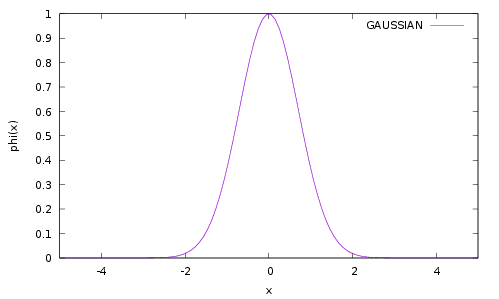
\includegraphics{gaussian}
\par\end{centering}
\caption{This figure depicts the Gaussian function $\sigma=1$ and $c=0$.\protect\label{fig:gaussian}}
\end{figure}
 From the graph above, one can conclude that the value of the function
rapidly approaches zero as the value of the variable $x$ moves away
from the center $c$. The training error of any given $R(x)$ RBF
network has as:
\begin{equation}
E\left(R\left(\overrightarrow{x}\right)\right)=\sum_{i=1}^{M}\left(R\left(\overrightarrow{x_{i}}\right)-y_{i}\right)^{2}\label{eq:RbfError}
\end{equation}
The set $\left(\overrightarrow{x_{i}},y_{i}\right),\ i=1,...,M$ denotes
the training set of the objective problem and the values $y_{i}$
are considered as the actual output for each pattern $\overrightarrow{x_{i}}$.

A magnitude of problems from the real world can be tackled using RBF
networks, such as face recognition \citep{rbfface}, numerical problems
\citep{rbfde1,rbfde2}, economic problems \citep{rbfstock}, robotics
\citep{rbfrobotics1,rbfrobotics2}, network security \citep{rbf_dos1,rbf_dos2},
classification of process faults \citep{rbf_process}, time series
prediction \citep{rbf_time}, estimation of wind power production
\citep{rbf_wind} etc. Moreover, Park et al. \citep{rbf_universal}
proved that an RBF network with one processing layer can be approximate
any given function.

This paper proposes a three-stage approach for the effective training
of RBF networks. The first stage of the method involves an algorithm
designed to efficiently determine the value ranges of the model parameters.
This detection is implemented using the K-Means algorithm \citep{kmeans}
for the weights and the variances of the radial functions. After applying
the above procedure, a range of values for the network parameters
is created which directly depends on the values produced by K-means
algorithm. During the second stage of the proposed work, a global
optimization procedure is incorporated to optimize the parameters
of the RBF network with respect to the equation \ref{eq:RbfError}.
The training of the network parameters is performed within the value
range of the first phase to avoid possible overfitting problems. In
the current work, the Genetic Algorithm is used as the method of the
second phase, but any optimization technique can be incorporated.
In the final phase of the proposed method, a local minimization technique
is applied to the optimal parameters obtained from the second phase.
The aim of the proposed method is first to determine a reliable range
of values for the parameters of RBF networks and then to train the
network parameters within this range, thereby avoiding potential arithmetic
instability issues associated with the conventional RBF training approach.

The proposed technique is the application of three distinct procedures
in series, where in each stage the results of the previous phase are
used. In the first phase, an initial estimation of the centers and
variances is performed with the method of K-Means. This method is
preferred because it is extremely fast to execute and can provide
an overview of the search space for neural networks. It is preferred
over using random values as this would require a significantly large
number of iterations for proper initialization of the parameters.
After applying the K-Means technique, a range of network parameter
values is generated, consisting of multiples of the values obtained
from the K-Means results.\textbf{ }In this way, on the one hand, the
use of the K-Means technique is utilized and, on the other hand, the
second-phase optimization algorithm is given the opportunity to search
for parameter values \LyXZeroWidthSpace that yield lower values of
the error function close to the initial values of the first phase.
A genetic algorithm is used as the optimization algorithm in the second
phase due to its adaptability to any environment and their widespread
use in many computational problems. However, any universal optimization
technique could be utilized in this phase. However, although genetic
algorithms are extremely effective methods of global optimization,
they often do not locate exactly a true minimum of the objective function
and therefore the help of a local minimization method is deemed necessary.
This occurs in the third phase, where a local optimization method
is applied to the chromosome with the smallest value produced in the
second phase. The minimum identified in this phase also represents
the final outcome of the algorithm, corresponding to a specific configuration
of the RBF network parameters.

The main features of the proposed method are its use of multiple techniques
in sequence to determine the optimal set of parameters for the machine
learning model while avoiding potential overfitting. In the first
discrete phase, a well-established clustering method, such as K-Means,
is employed to identify a promising range of values for the model
parameters. In the second phase, a global optimization algorithm is
applied to minimize the error function within the bounds established
in the first phase. Finally, in the last phase, a local minimization
method is used to locate a guaranteed local minimum of the error function.
This final phase ensures that the network parameters are trained within
the value range determined in the first phase.

The rest of this paper has the following structure: in section \ref{sec:Materials-and-Methods},
the parts of the proposed technique are presented in detail, in section
\ref{sec:Results}, the datasets on which the method was applied are
presented, as well as the experimental results from its application,
and in section \ref{sec:Conclusions}, an extensive discussion of
the practical results of the proposed technique is made and possible
weaknesses that arose during the execution of the experiments are
analyzed.

\section{Materials and Methods\protect\label{sec:Materials-and-Methods}}

The three distinct phases of the proposed method are discussed here.
The discussion initiates with the first phase, where the construction
of the ranges for the parameter values is performed using the K-means
algorithm. Afterwards, the steps of the used Genetic Algorithm are
presented in detail and finally, this section concludes with the description
of the final phase, where a local optimization method is applied to
the best located chromosome of the second phase. Also, the description
of the used datasets is provided in this section in table format.

\subsection{Related work}

Over the past years, numerous techniques have been proposed for training
neural networks and efficiently adapting their parameters. Among these,
there are methods specifically designed for the effective initialization
of RBF network parameters \citep{rbfinit1,rbfinit2,rbfinit3}. Moreover,
Benoudjit et al. discussed on the estimation of kernels in these models
\citep{rbfkernel}. Additionally, a series of pruning techniques \citep{rbfprun1,rbfprun2,rbfprun3}
have been introduced aiming to reduce the required number of parameters
for networks, providing a solution to the overfitting problem. Also,
methods that construct the architecture of RBF networks have been
proposed recently, such as the work of Du et al. \citep{rbfcon1}
or the work of Yu et al. who suggested an incremental design framework
for RBF networks \citep{rbfcon2}. Also, a series of optimization
techniques have been used in the past for the minimization of equation
\ref{eq:RbfError}, such as genetic algorithms \citep{rbfga1,rbfga2},
the Particle Swarm Optimization method \citep{rbfpso1,rbfpso2}, the
Differential Evolution technique \citep{rbfdiff1} etc. Moreover,
the rapid growth in the use of parallel computing techniques in recent
decades has led to the publication of numerous scientific studies
that leverage these methods \citep{rbfpar1,rbfpar2}. Recently, Rani
et al. proposed an improved PSO optimizer that integrates a differential
search mechanism for efficient RBF network training \citep{rbf_pso_new}.
Moreover, Karamichailidou et al. suggested a novel method for RBF
training using variable projection and fuzzy means \citep{rbf_variable_projection}.

\subsection{The description of the first phase}

The method of K-means, used widely in machine learning, is incorporated
in the first phase for the location of the ranges for the centers
and variances of the model. This method is incorporated to locate
the centers and the variances of the possible groups of a series of
points. Furthermore, a series of extensions of this method have been
published during the past years, such as the Genetic K-means algorithm
\citep{gen_kmeans}, the unsupervised K-means algorithm \citep{unsuper_kmeans},
the Fixed-centered K-means algorithm \citep{fixed_kmeans} etc. A
detailed review of the K-means method can be located in the paper
published by Oti et al. \citep{kmeans_review}. The K-means method
is presented in Algorithm \ref{alg:The-K-Means-algorithm.}. A graphical
rerpesentation is provided in Figure \ref{fig:kmeans}.

\begin{algorithm}[H]
\caption{The procedure of the K-Means algorithm.\protect\label{alg:The-K-Means-algorithm.}}

\begin{enumerate}
\item \textbf{Input: }The set of patterns of the objective problem\textbf{
$\left(\overrightarrow{x_{i}}\right),\ i=1,...,M$}
\item \textbf{Input}: the number of centers $k$.
\item \textbf{Output}: The vectors $\overrightarrow{c_{i}},\ i=1,..,k$
and the quantities $\sigma_{i},\ i=1,\ldots,k$
\item \textbf{Set} $S_{j}=\left\{ \right\} ,\ j=1..k$, as the sets of samples
belonging to the same group.
\item \textbf{For} every pattern $x_{i},\ i=1,...,M$ \textbf{do\label{enu:For-every-pattern}}
\begin{enumerate}
\item \textbf{Set} $j^{*}=\min_{i=1}^{k}\left\{ D\left(x_{i},c_{j}\right)\right\} $.
\item \textbf{Set} $S_{j^{*}}=S_{j^{*}}\cup\left\{ x_{i}\right\} $.
\end{enumerate}
\item \textbf{EndFor}
\item \textbf{For} each center $c_{j},\ j=1..k$ \textbf{do}
\begin{enumerate}
\item The\textbf{ }number\textbf{ }$M_{j}$ \textbf{represents} the number
of patterns that have been assigned to cluster $S_{j}$
\item \textbf{Compute }$c_{j}$ as
\[
c_{j}=\frac{1}{M_{j}}\sum_{i=1}^{M_{j}}x_{i}
\]
\end{enumerate}
\item \textbf{EndFor}
\item \textbf{Calculate} the quantities $s_{j}$ as 
\[
\sigma_{j}^{2}=\frac{\sum_{i=1}^{M_{j}}\left(x_{i}-c_{j}\right)^{2}}{M_{j}}
\]
\item The method will \textbf{terminate} when there is no longer a significant
change in the center values $c_{i}$ from iteration to iteration.
\item \textbf{Go to} step \ref{enu:For-every-pattern}.
\end{enumerate}
\end{algorithm}
\begin{figure}[H]
\begin{centering}
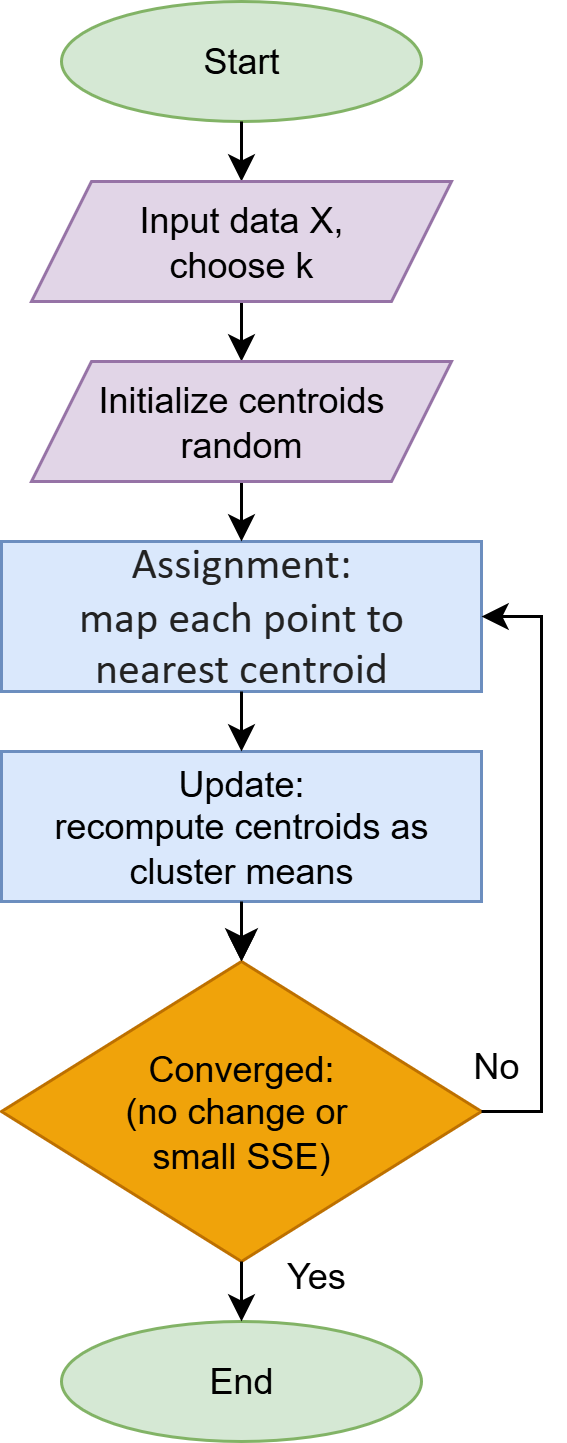
\includegraphics[scale=0.75]{kmeans_flowchart}
\par\end{centering}
\caption{A graphical presentation of the K-means algorithm. \protect\label{fig:kmeans}}
\end{figure}

After the calculation of $\overrightarrow{c_{i}},\ i=1,..,k$ and
the quantities $\sigma_{i},\ i=1,\ldots,k$, the method locates the
margin vectors $\overrightarrow{L},\ \overrightarrow{R}$ for the
parameters of the RBF network. The dimension of the bound vectors
is defined as:
\begin{equation}
n=(d+2)\times k\label{eq:bound_dimension}
\end{equation}

The algorithm is depicted graphically in Figure \ref{fig:The-bound-construction}
describes a procedure for computing safe parameter bounds informed
by K-means. The process begins by preparing the inputs the cluster
centroids and spreads, a positive initial bound for the weights, and
a scaling factor $F\ge1$ aiming to produce the lower and upper bound
vectors $L$ and $R$. For each group and for each of its features,
symmetric bounds around zero are computed as $F$ times the corresponding
centroid coordinate (i.e., $L_{m}=-F\times c_{ij},\ R_{m}=F\times c_{ij}$).
After completing a group’s features, a complementary step computes
bounds based on that group’s spread, using $F\times\sigma_{i}$ (i.e.,
$L_{m}=-F\times\sigma_{i},\ R_{m}=F\times\sigma_{i}$). In this way,
every group receives a complete, consistent specification through
two contributions: one driven by feature centroids and one capturing
group extent. Once all groups have been processed, initial bounds
for the combining weights are assigned using a fixed symmetric limit
$B_{w}$ (i.e., $L_{m}=-B_{w},\ R_{m}=B_{w}$). Finally, all computed
limits are assembled into L and R, ready for training, estimation,
or validity checks. The overall logic is hierarchical and layered:
leveraging centroid information, incorporating spread, and bounding
the weights, with clear and reproducible steps throughout the flow.

\begin{figure}[H]
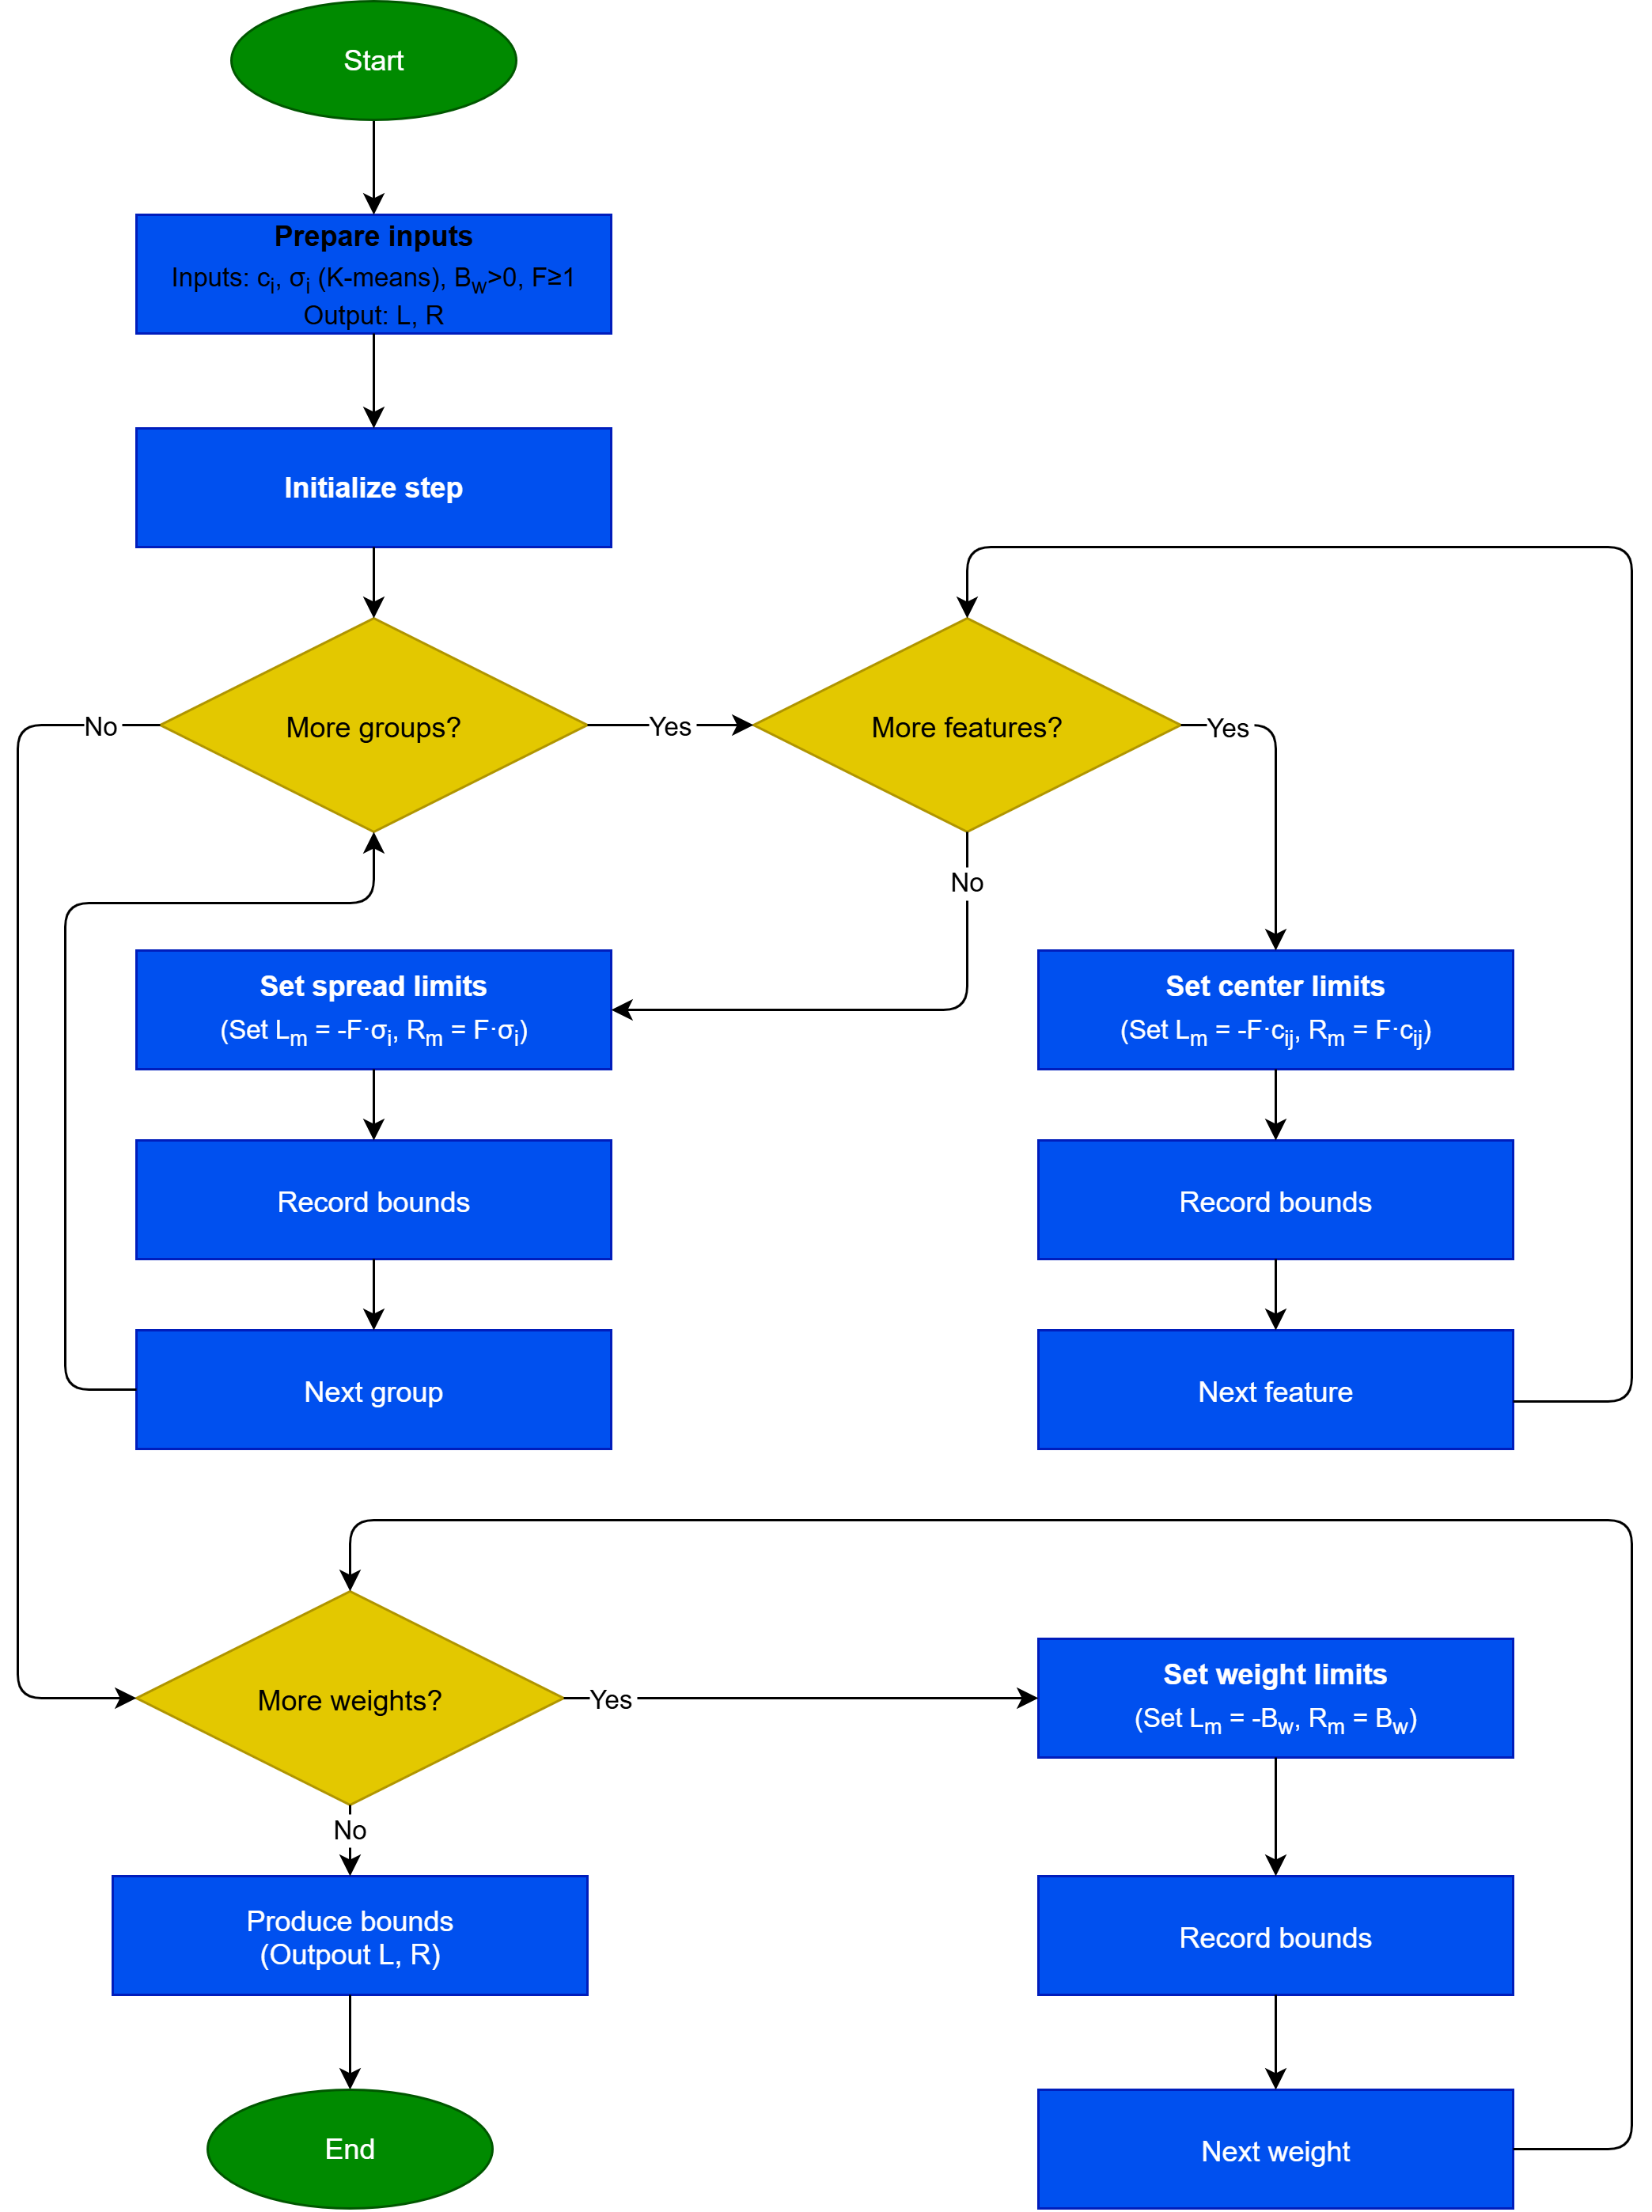
\includegraphics[scale=0.5]{flowchart2}

\caption{The bound construction algorithm.\protect\label{fig:The-bound-construction}}

\end{figure}


\subsection{The description for the second phase}

During the second phase, an optimization procedure is utilized to
minimize the equation \ref{eq:RbfError} considering the bound vectors
$\overrightarrow{L},\ \overrightarrow{R}$ of the previous phase.
In the proposed implementation, the Genetic Algorithm was incorporated
during the second phase. Genetic algorithms are evolutionary methods
that are based on randomly produced solutions of the objective problem.\textbf{
}The candidate solutions in a genetic algorithm are typically referred
to as chromosomes, and they evolve through operations inspired by
natural processes, such as selection, crossover, and mutation. They
have been incorporated in a wide series of problems, such as energy
problems \citep{gen_app1}, water distribution \citep{gen_app2},
problems appearing in banking transactions \citep{gen_app3}, optimization
of neural networks \citep{gen_app4} etc. Also, another advantage
of Genetic Algorithms is that they can easily adopt parallel programming
techniques in order to speed up the evolutionary process \citep{pga1,pga2}.
Figure \ref{fig:The-layout-of} illustrates the structure of the chromosomes
involved in the genetic algorithm at this phase. In this figure the
following assumptions hold:
\begin{enumerate}
\item The value $c_{i,j}$ denotes the $j$ element of the $i$ center of
the RBF network, with $i\in[1,k]$ and $j\in[1,d].$
\item The value $\sigma_{i}$ represents the $\sigma$ parameter for the
corresponding radial function.
\item The value $w_{i},\ i\in[1,k]$ represents the weight for the corresponding
radial function.
\end{enumerate}
\begin{figure}[H]
\begin{raggedright}
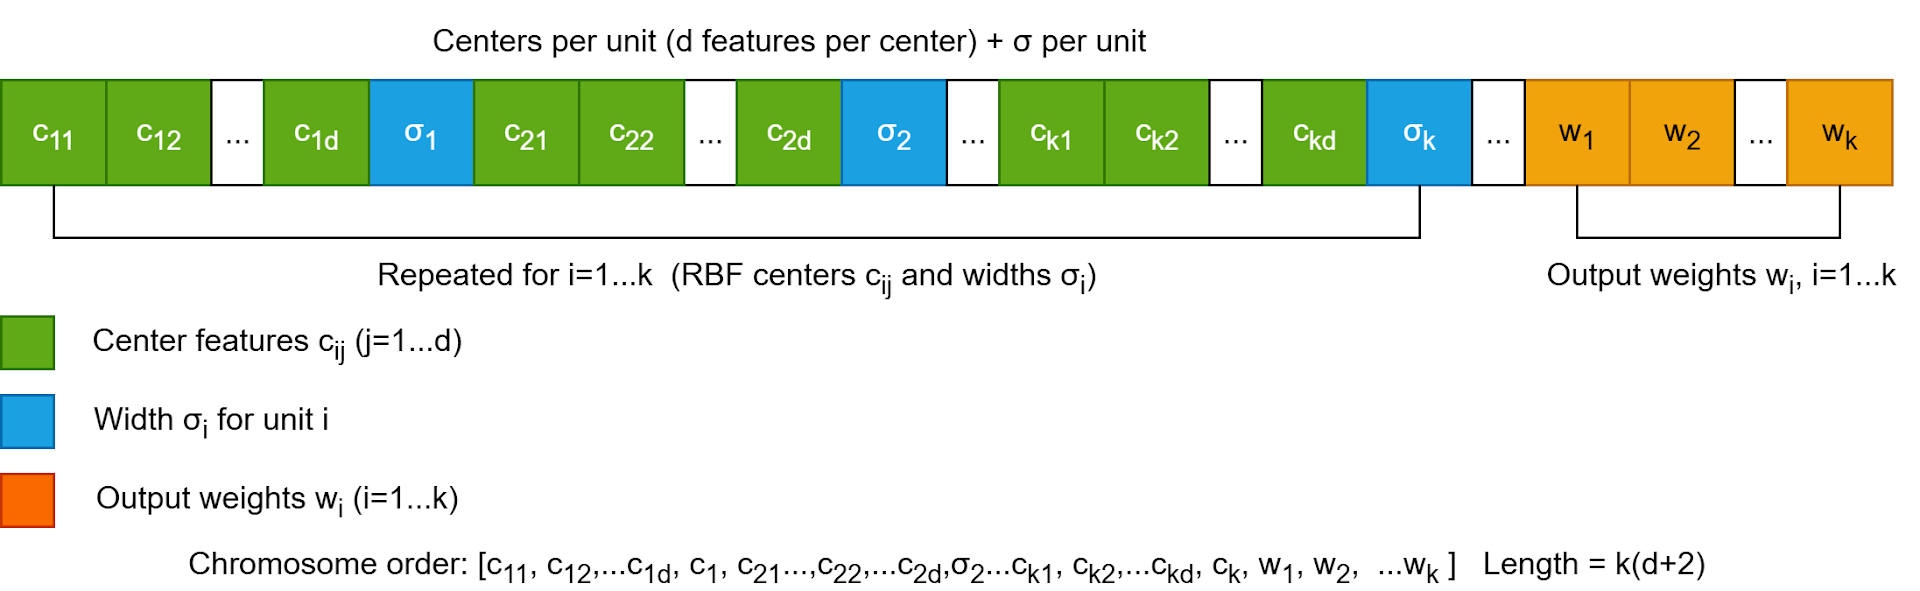
\includegraphics[scale=0.2]{chrom_layout}
\par\end{raggedright}
\caption{The figure illustrates the schematic arrangement of a chromosome in
the proposed genetic algorithm.\protect\label{fig:The-layout-of}}
\end{figure}

The following steps outline the proposed genetic algorithm:
\begin{enumerate}
\item \textbf{Initialization step}. 
\begin{enumerate}
\item The following set of parameter are\textbf{ initialized:} $N_{c}$
for the number of chromosomes, $N_{g}$ used to express the maximum
number of allowed generations, $p_{s}$ that defines the selection
rate and finally $p_{m}$ which is used to represent the mutation
rate.
\item The chromosomes in the proposed genetic algorithm are \textbf{initialized}
as random decimal numbers that follow the configuration of Figure
\ref{fig:The-layout-of} and the initialization is performed within
the value range of the first phase which is defined by the vectors\textbf{
}$\overrightarrow{L},\ \overrightarrow{R}$.
\item \textbf{Set} $k=0$. This variable denotes the number of generations.
\end{enumerate}
\item \textbf{Fitness calculation step}.
\begin{enumerate}
\item \textbf{For} $i=1,\ldots,N_{c}$ \textbf{do}
\begin{enumerate}
\item \textbf{Produce }an RBF network $R_{i}=R\left(\overrightarrow{x},\overrightarrow{g_{i}}\right).$
The parameters of this network are stored in the chromosome $\overrightarrow{g_{i}}.$
\item \textbf{Estimate} the related fitness $f_{i}$ as\textbf{
\begin{equation}
f_{i}=\sum_{j=1}^{M}\left(R\left(\overrightarrow{x}_{j},\overrightarrow{g_{i}}\right)-y_{j}\right)^{2}\label{eq:eq1-1}
\end{equation}
}
\end{enumerate}
\item \textbf{End For}
\end{enumerate}
\item \textbf{Genetic operations step}.
\begin{enumerate}
\item Selection procedure: Initially, all chromosomes are sorted based on
their fitness values. The top $p_{s}\times N_{c}$ chromosomes are
directly carried over to the next generation without any modification.
The remaining individuals are replaced by offspring generated through
crossover and mutation operations.
\item Crossover procedure: During this procedure In this procedure $\left(1-p_{s}\right)\times N_{c}$
new chromosomes will be constructed. For each pair $\left(\tilde{z},\tilde{w}\right)$
of new chromosomes, two chromosomes $(z,w)$ are chosen using tournament
selection. The new offsprings are produced following the scheme:
\begin{eqnarray}
\tilde{z_{i}} & = & a_{i}z_{i}+\left(1-a_{i}\right)w_{i}\nonumber \\
\tilde{w_{i}} & = & a_{i}w_{i}+\left(1-a_{i}\right)z_{i}\label{eq:crossover_ali-1}
\end{eqnarray}
The numbers $a_{i}$ are considered random numbers in the range $[-0.5,1.5]$
\citep{kaelo}. 
\item Mutation procedure: A random number $r\in[0,1]$ is picked for each
element $t_{j},j=1,\ldots,n$ and for every chromosome $g_{i}$ .
If $r\le p_{m}$ , then this element is altered according to the following
equation:
\begin{equation}
t'_{j}=\begin{cases}
t_{j}+\Delta\left(k,R_{j}-t_{j}\right), & t=0\\
t_{j}-\Delta\left(k,t_{j}-L_{j}\right), & t=1
\end{cases}\label{eq:delta1}
\end{equation}
The value $t$ is a random number that can be either 0 or 1. The function
function $\Delta(k,y)$ is provided by the following equation:
\begin{equation}
\Delta(k,y)=y\left(1-r^{\left(1-\frac{k}{N_{g}}\right)}\right)\label{eq:delta2}
\end{equation}
\end{enumerate}
\item \textbf{Termination check step}.
\begin{enumerate}
\item \textbf{Set} $k=k+1$
\item \textbf{If} $k<N_{g}$ then the procedure returns to the Fitness Calculation
step.
\item \textbf{Otherwise}, the best chromosome $g^{*}$ is returned as the
result of the algorithm.
\end{enumerate}
\end{enumerate}

\subsection{The steps of the third phase}

In the third phase of the present work, a local optimization procedure
is applied to the results of the previous phase to identify an actual
minimum of the RBF network’s training error.\textbf{ }In this work,
a BFGS variant of Powell \citep{powell} was utilized as the local
optimization method. This variant can preserve the bounds located
previously in an efficient way. During the past years a series of
modifications to the BFGS method have been introduced, such as the
limited memory variant L-BFGS ideal for large scale problems \citep{lbfgs}
or the Regularized Stochastic BFGS Algorithm \citep{resbfgs}. Also,
Dai published an article on the convergence properties of the BFGS
method \citep{conbfgs}. The main steps of the final phase of the
algorithm are:
\begin{enumerate}
\item \textbf{Get} the best chromosome $\overrightarrow{g^{*}}$ of the
previous phase.
\item \textbf{Produce} the RBF network that corresponds to this chromosome
and denoted as $R^{*}=R\left(\overrightarrow{x},\overrightarrow{g^{*}}\right)$.
\item \textbf{Minimize} the training error of the network $R^{*}$ using
the local search procedure of this phase.
\item The network $R^{*}$ is \textbf{applied} to the test set and the corresponding
classification or regression error is calculated and reported.
\end{enumerate}
A summary flow chart showing the sequence of the various phases of
the proposed work is presented in Figure \ref{fig:summary}.

\begin{figure}[H]
\begin{centering}
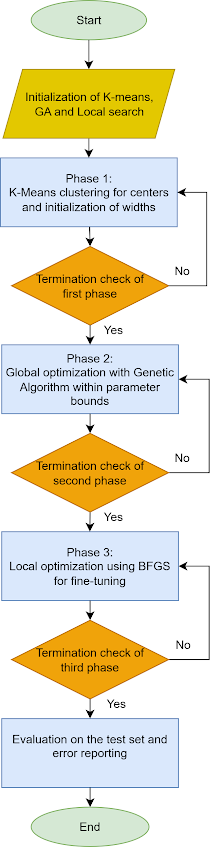
\includegraphics[scale=0.5]{overall_flowchart}
\par\end{centering}
\caption{Summary flowchart of the proposed method.\protect\label{fig:summary}}

\end{figure}


\subsection{The experimental datasets.}

The proposed method was evaluated on a broad set of classification
and regression problems, available from the UCI database \citep{uci},
the KEEL database \citep{Keel}, and the STATLIB database \citep{statlib}.
The classification datasets used in the experiments, along with their
details (number of patterns and classes), are summarized in Table
\ref{tab:classData}.

\begin{table}[H]
\caption{The column 'DATASET' indicates the name of each dataset. The 'Reference
Paper' column refers to the publication in which the dataset was mentioned.
The 'Patterns' column shows the number of patterns in the dataset,
while the 'Number of Classes' column represents the number of distinct
classes contained in the dataset.\protect\label{tab:classData}}

\centering{}%
\begin{tabular}{|c|c|c|c|}
\hline 
DATASET & Reference paper & Patterns & Number of Classes\tabularnewline
\hline 
\hline 
APPENDICITIS & \citep{appendicitis} & 106 & 2\tabularnewline
\hline 
ALCOHOL & \citep{alcohol} & 476 & 4\tabularnewline
\hline 
AUSTRALIAN & \citep{australian} & 690 & 2\tabularnewline
\hline 
BALANCE & \citep{balance} & 625 & 3\tabularnewline
\hline 
CLEVELAND & \citep{cleveland1,cleveland2} & 297 & 5\tabularnewline
\hline 
CIRCULAR & \citep{fcgen} & 500 & 2\tabularnewline
\hline 
DERMATOLOGY & \citep{dermatology} & 368 & 6\tabularnewline
\hline 
ECOLI & \citep{ecoli} & 336 & 8\tabularnewline
\hline 
HAYES ROTH & \citep{hayes-roth} & 132 & 3\tabularnewline
\hline 
HEART & \citep{heart} & 270 & 2\tabularnewline
\hline 
HEARTATTACK & \citep{heartAttack} & 303 & 2\tabularnewline
\hline 
HOUSEVOTES & \citep{housevotes} & 232 & 2\tabularnewline
\hline 
IONOSPHERE & \citep{ion1,ion2} & 351 & 2\tabularnewline
\hline 
LIVERDISORDER & \citep{liver,liver1} & 345 & 2\tabularnewline
\hline 
LYMOGRAPHY & \citep{lymography} & 148 & 4\tabularnewline
\hline 
MAMMOGRAPHIC & \citep{mammographic} & 830 & 2\tabularnewline
\hline 
PARKINSONS & \citep{parkinsons1,parkinsons2} & 195 & 2\tabularnewline
\hline 
PIMA & \citep{pima} & 768 & 2\tabularnewline
\hline 
POPFAILURES & \citep{popfailures} & 540 & 2\tabularnewline
\hline 
REGIONS2 & \citep{regions2} & 622 & 5\tabularnewline
\hline 
SAHEART & \citep{saheart} & 462 & 2\tabularnewline
\hline 
SEGMENT & \citep{segment} & 2300 & 7\tabularnewline
\hline 
SPIRAL & \citep{fcgen} & 2000 & 2\tabularnewline
\hline 
STATHEART & \citep{statheart} & 270 & 2\tabularnewline
\hline 
STUDENT & \citep{student} & 403 & 2\tabularnewline
\hline 
TRANSFUSION & \citep{transfusion} & 748 & 2\tabularnewline
\hline 
WDBC & \citep{wdbc1,wdbc2} & 569 & 2\tabularnewline
\hline 
WINE & \citep{wine1,wine2} & 179 & 3\tabularnewline
\hline 
Z\_F\_S & \citep{eeg1,eeg2} & 300 & 3\tabularnewline
\hline 
Z\_O\_N\_F\_S & \citep{eeg1,eeg2} & 500 & 5\tabularnewline
\hline 
ZO\_NF\_S & \citep{eeg1,eeg2} & 500 & 3\tabularnewline
\hline 
ZONF\_S & \citep{eeg1,eeg2} & 500 & 2\tabularnewline
\hline 
ZOO & \citep{zoo} & 101 & 7\tabularnewline
\hline 
\end{tabular}
\end{table}

Also, table \ref{tab:regressionDatasets} presents the used regression
datasets.

\begin{table}[H]

\caption{The list of regression datasets.\protect\label{tab:regressionDatasets}}

\centering{}%
\begin{tabular}{|c|c|c|}
\hline 
DATASET & Reference paper & Patterns\tabularnewline
\hline 
\hline 
ABALONE & \citep{abalone} & 4177\tabularnewline
\hline 
AIRFOIL & \citep{airfoil} & 1483\tabularnewline
\hline 
AUTO & \citep{auto_dataset} & 392\tabularnewline
\hline 
BK & \citep{fcgen} & 96\tabularnewline
\hline 
BL & \citep{fcgen} & 43\tabularnewline
\hline 
BASEBALL & \citep{Keel} & 337\tabularnewline
\hline 
CONCRETE & \citep{concrete} & 1030\tabularnewline
\hline 
DEE & \citep{Keel} & 365\tabularnewline
\hline 
FA & \citep{statlib} & 252\tabularnewline
\hline 
FRIEDMAN & \citep{friedman} & 1200\tabularnewline
\hline 
FY & \citep{statlib} & 125\tabularnewline
\hline 
HO & \citep{statlib} & 506\tabularnewline
\hline 
HOUSING & \citep{housing} & 506\tabularnewline
\hline 
LASER & \citep{uci} & 993\tabularnewline
\hline 
LW & \citep{statlib} & 189\tabularnewline
\hline 
MORTGAGE & \citep{Keel} & 1049\tabularnewline
\hline 
PL & \citep{statlib} & 1650\tabularnewline
\hline 
PLASTIC & \citep{uci} & 1670\tabularnewline
\hline 
QUAKE & \citep{uci} & 2178\tabularnewline
\hline 
SN & \citep{statlib} & 576\tabularnewline
\hline 
STOCK & \citep{Keel} & 950\tabularnewline
\hline 
TREASURY & \citep{Keel} & 1049\tabularnewline
\hline 
\end{tabular}
\end{table}


\section{Results\protect\label{sec:Results}}

\subsection{Experimental results }

The experiments were conducted on a Debian Linux system with 128\,GB
of RAM, and all the necessary code was implemented in the C++ programming
language.\textbf{ }Also, the OPTIMUS computing environment \citep{optimus},
available from \url{https://github.com/itsoulos/GlobalOptimus.git}
(accessed on 9 October 2025) was used for the optimization methods.
Ten-fold cross-validation was employed to validate the experimental
results. The average classification error is calculated as: 
\begin{equation}
E_{C}\left(N\left(\overrightarrow{x},\overrightarrow{w}\right)\right)=100\times\frac{\sum_{i=1}^{N}\left(\mbox{class}\left(N\left(\overrightarrow{x_{i}},\overrightarrow{w}\right)\right)-y_{i}\right)}{N}
\end{equation}
The set $T$ denotes the associated test set, where $T=\left(x_{i},y_{i}\right),\ i=1,\ldots,N$.
Similarly, the average regression error has the following definition:
\begin{equation}
E_{R}\left(N\left(\overrightarrow{x},\overrightarrow{w}\right)\right)=\frac{\sum_{i=1}^{N}\left(N\left(\overrightarrow{x_{i}},\overrightarrow{w}\right)-y_{i}\right)^{2}}{N}
\end{equation}
Table \ref{tab:settings} contains the values for each parameter of
this method. 
\begin{table}[H]
\caption{The values for each parameter of the proposed method.\protect\label{tab:settings}}

\centering{}%
\begin{tabular}{|c|c|c|}
\hline 
NAME & MEANING & VALUE\tabularnewline
\hline 
\hline 
$k$ & Number of radial functions & $10$\tabularnewline
\hline 
$F$ & Scaling factor & $2.0$\tabularnewline
\hline 
$B_{w}$ & Bound value for the weights & $10.0$\tabularnewline
\hline 
$N_{c}$ & Chromosomes & $500$\tabularnewline
\hline 
$N_{g}$ & Allowed number of generations & $200$\tabularnewline
\hline 
$p_{s}$ & Selection rate & $0.1$\tabularnewline
\hline 
$p_{m}$ & Mutation rate & $0.05$\tabularnewline
\hline 
\end{tabular}
\end{table}
 In the results tables that follow, the columns and rows have the
following meaning:
\begin{enumerate}
\item The column DATASET is used to represent the name of the used dataset.
\item The results from the incorporation of the BFGS procedure \citep{bfgs}
to train an artificial neural network \citep{nn1,nn2} with 10 weights
are presented in column under the title BFGS.
\item The ADAM column presents the results obtained by training a 10-weight
neural network using the ADAM local optimization technique \citep{Adam,AdamNN}.
\item The column RBF-KMEANS is used here to denote the usage of the initial
training method of RBF networks to train an RBF network with 10 nodes.
\item The column NEAT (NeuroEvolution of Augmenting Topologies) \citep{neat}
stands for the method NEAT incorporated in the training of neural
networks.
\item The column DNN stands for the incorporation of a deep neural network
as implemented in the Tiny Dnn library, that can be downloaded freely
from \url{https://github.com/tiny-dnn/tiny-dnn}(accessed on 9 October
2025). The optimization method AdaGrad \citep{adagrad} was incorporated
for the training of the neural network.
\item The BAYES column presents results obtained using the Bayesian optimizer
from the open-source BayesOpt library \citep{bayesopt}, applied to
train a neural network with 10 processing nodes.
\item The column GENRBF stands method introduced in \citep{rbf_gen1} for
RBF training.
\item The column PROPOSED is used to represent the results obtained by the
current work.
\item The row denoted as AVERAGE summarizes the mean regression or classification
error calculated over all datasets.
\item In the experimental results, boldface highlighting was used to make
it clear which of the machine learning techniques has the lowest error
on each dataset..
\end{enumerate}
\begin{table}[H]
\caption{The experimental outcomes on the classification datasets achieved
with the machine learning techniques presented in this section.\protect\label{tab:expClass}}

\centering{}{\footnotesize{}%
\begin{tabular}{|c|c|c|c|c|c|c|c|c|}
\hline 
{\scriptsize\textbf{DATASET}} & {\footnotesize\textbf{BFGS}} & {\footnotesize\textbf{ADAM}} & {\footnotesize\textbf{NEAT}} & {\footnotesize\textbf{DNN}} & {\footnotesize\textbf{BAYES}} & {\footnotesize\textbf{RBF-KMEANS}} & {\footnotesize\textbf{GENRBF}} & {\footnotesize\textbf{PROPOSED}}\tabularnewline
\hline 
\hline 
{\scriptsize Alcohol} & {\footnotesize 41.50\%} & {\footnotesize 57.78\%} & {\footnotesize 66.80\%} & {\footnotesize 39.04\%} & {\footnotesize 30.85\%} & {\footnotesize 49.38\%} & {\footnotesize 52.45\%} & {\footnotesize\textbf{28.57\%}}\tabularnewline
\hline 
{\scriptsize Appendicitis} & {\footnotesize 18.00\%} & {\footnotesize 16.50\%} & {\footnotesize 17.20\%} & {\footnotesize 17.30\%} & {\footnotesize 15.00\%} & {\footnotesize\textbf{12.23\%}} & {\footnotesize 16.83\%} & {\footnotesize 15.00\%}\tabularnewline
\hline 
{\scriptsize Australian} & {\footnotesize 38.13\%} & {\footnotesize 35.65\%} & {\footnotesize 31.98\%} & {\footnotesize 35.03\%} & {\footnotesize 34.83\%} & {\footnotesize 34.89\%} & {\footnotesize 41.79\%} & {\footnotesize\textbf{22.67\%}}\tabularnewline
\hline 
{\scriptsize Balance} & {\footnotesize 8.64\%} & {\footnotesize\textbf{7.87\%}} & {\footnotesize 23.14\%} & {\footnotesize 24.56\%} & {\footnotesize 8.13\%} & {\footnotesize 33.42\%} & {\footnotesize 38.02\%} & {\footnotesize 13.11\%}\tabularnewline
\hline 
{\scriptsize Cleveland} & {\footnotesize 77.55\%} & {\footnotesize 67.55\%} & {\footnotesize 53.44\%} & {\footnotesize 63.28\%} & {\footnotesize 64.79\%} & {\footnotesize 67.10\%} & {\footnotesize 67.47\%} & {\footnotesize\textbf{50.86\%}}\tabularnewline
\hline 
{\scriptsize Circular} & {\footnotesize 6.08\%} & {\footnotesize 19.95\%} & {\footnotesize 35.18\%} & {\footnotesize 21.87\%} & {\footnotesize 21.06\%} & {\footnotesize 5.98\%} & {\footnotesize 21.43\%} & {\footnotesize\textbf{5.13\%}}\tabularnewline
\hline 
{\scriptsize Dermatology} & {\footnotesize 52.92\%} & {\footnotesize 26.14\%} & {\footnotesize 32.43\%} & {\footnotesize\textbf{24.26\%}} & {\footnotesize 49.80\%} & {\footnotesize 62.34\%} & {\footnotesize 61.46\%} & {\footnotesize 36.00\%}\tabularnewline
\hline 
{\scriptsize Hayes Roth} & {\footnotesize\textbf{37.33\%}} & {\footnotesize 59.70\%} & {\footnotesize 50.15\%} & {\footnotesize 44.65\%} & {\footnotesize 59.39\%} & {\footnotesize 64.36\%} & {\footnotesize 63.46\%} & {\footnotesize 38.31\%}\tabularnewline
\hline 
{\scriptsize Heart} & {\footnotesize 39.44\%} & {\footnotesize 38.53\%} & {\footnotesize 39.27\%} & {\footnotesize 30.67\%} & {\footnotesize 30.85\%} & {\footnotesize 31.20\%} & {\footnotesize 28.44\%} & {\footnotesize\textbf{16.07\%}}\tabularnewline
\hline 
{\scriptsize HeartAttack} & {\footnotesize 46.67\%} & {\footnotesize 45.55\%} & {\footnotesize 32.34\%} & {\footnotesize 32.97\%} & {\footnotesize 33.93\%} & {\footnotesize 29.00\%} & {\footnotesize 40.48\%} & {\footnotesize\textbf{19.20\%}}\tabularnewline
\hline 
{\scriptsize HouseVotes} & {\footnotesize 7.13\%} & {\footnotesize 7.48\%} & {\footnotesize 10.89\%} & {\footnotesize\textbf{3.13\%}} & {\footnotesize 8.39\%} & {\footnotesize 6.13\%} & {\footnotesize 11.99\%} & {\footnotesize 3.65\%}\tabularnewline
\hline 
{\scriptsize Ionosphere} & {\footnotesize 15.29\%} & {\footnotesize 16.64\%} & {\footnotesize 19.67\%} & {\footnotesize 12.57\%} & {\footnotesize 15.03\%} & {\footnotesize 16.22\%} & {\footnotesize 19.83\%} & {\footnotesize\textbf{12.17\%}}\tabularnewline
\hline 
{\scriptsize Liverdisorder} & {\footnotesize 42.59\%} & {\footnotesize 41.53\%} & {\footnotesize 30.67\%} & {\footnotesize 32.21\%} & {\footnotesize 34.21\%} & {\footnotesize 30.84\%} & {\footnotesize 36.97\%} & {\footnotesize\textbf{29.29\%}}\tabularnewline
\hline 
{\scriptsize Lymography} & {\footnotesize 35.43\%} & {\footnotesize 29.26\%} & {\footnotesize 33.70\%} & {\footnotesize\textbf{24.07\%}} & {\footnotesize 25.50\%} & {\footnotesize 25.50\%} & {\footnotesize 29.33\%} & {\footnotesize 24.36\%}\tabularnewline
\hline 
{\scriptsize Mammographic} & {\footnotesize\textbf{17.24\%}} & {\footnotesize 46.25\%} & {\footnotesize 22.85\%} & {\footnotesize 19.83\%} & {\footnotesize 21.15\%} & {\footnotesize 21.38\%} & {\footnotesize 30.41\%} & {\footnotesize 17.79\%}\tabularnewline
\hline 
{\scriptsize Parkinsons} & {\footnotesize 27.58\%} & {\footnotesize 24.06\%} & {\footnotesize 18.56\%} & {\footnotesize 21.32\%} & {\footnotesize 19.32\%} & {\footnotesize\textbf{17.41\%}} & {\footnotesize 33.81\%} & {\footnotesize 17.53\%}\tabularnewline
\hline 
{\scriptsize Pima} & {\footnotesize 35.59\%} & {\footnotesize 34.85\%} & {\footnotesize 34.51\%} & {\footnotesize 32.63\%} & {\footnotesize 35.52\%} & {\footnotesize 25.78\%} & {\footnotesize 27.83\%} & {\footnotesize\textbf{24.02\%}}\tabularnewline
\hline 
{\scriptsize Popfailures} & {\footnotesize 5.24\%} & {\footnotesize\textbf{5.18\%}} & {\footnotesize 7.05\%} & {\footnotesize 6.83\%} & {\footnotesize 7.63\%} & {\footnotesize 7.04\%} & {\footnotesize 7.08\%} & {\footnotesize 6.33\%}\tabularnewline
\hline 
{\scriptsize Regions2} & {\footnotesize 36.28\%} & {\footnotesize 29.85\%} & {\footnotesize 33.23\%} & {\footnotesize 33.42\%} & {\footnotesize 30.16\%} & {\footnotesize 38.29\%} & {\footnotesize 39.98\%} & {\footnotesize\textbf{26.29\%}}\tabularnewline
\hline 
{\scriptsize Saheart} & {\footnotesize 37.48\%} & {\footnotesize 34.04\%} & {\footnotesize 34.51\%} & {\footnotesize 35.11\%} & {\footnotesize 34.87\%} & {\footnotesize 32.19\%} & {\footnotesize 33.90\%} & {\footnotesize\textbf{28.50\%}}\tabularnewline
\hline 
{\scriptsize Segment} & {\footnotesize 68.97\%} & {\footnotesize 49.75\%} & {\footnotesize 66.72\%} & {\footnotesize\textbf{32.04\%}} & {\footnotesize 51.70\%} & {\footnotesize 59.68\%} & {\footnotesize 54.25\%} & {\footnotesize 45.00\%}\tabularnewline
\hline 
{\scriptsize Sonar} & {\footnotesize 25.85\%} & {\footnotesize 30.33\%} & {\footnotesize 34.10\%} & {\footnotesize\textbf{20.50\%}} & {\footnotesize 27.15\%} & {\footnotesize 27.90\%} & {\footnotesize 37.13\%} & {\footnotesize 22.00\%}\tabularnewline
\hline 
{\scriptsize Spiral} & {\footnotesize 47.99\%} & {\footnotesize 48.90\%} & {\footnotesize 50.22\%} & {\footnotesize 45.64\%} & {\footnotesize 50.57\%} & {\footnotesize 44.87\%} & {\footnotesize 50.02\%} & {\footnotesize\textbf{13.26\%}}\tabularnewline
\hline 
{\scriptsize Statheart} & {\footnotesize 39.65\%} & {\footnotesize 44.04\%} & {\footnotesize 44.36\%} & {\footnotesize 30.22\%} & {\footnotesize 31.41\%} & {\footnotesize 31.36\%} & {\footnotesize 42.94\%} & {\footnotesize\textbf{19.67\%}}\tabularnewline
\hline 
{\scriptsize Student} & {\footnotesize 7.14\%} & {\footnotesize\textbf{5.13\%}} & {\footnotesize 10.20\%} & {\footnotesize 6.93\%} & {\footnotesize 5.83\%} & {\footnotesize 5.49\%} & {\footnotesize 33.26\%} & {\footnotesize 5.23\%}\tabularnewline
\hline 
{\scriptsize Transfusion} & {\footnotesize 25.84\%} & {\footnotesize 25.68\%} & {\footnotesize\textbf{24.87\%}} & {\footnotesize 25.92\%} & {\footnotesize 25.41\%} & {\footnotesize 26.41\%} & {\footnotesize 25.67\%} & {\footnotesize 26.04\%}\tabularnewline
\hline 
{\scriptsize Wdbc} & {\footnotesize 29.91\%} & {\footnotesize 35.35\%} & {\footnotesize 12.88\%} & {\footnotesize 9.43\%} & {\footnotesize 9.52\%} & {\footnotesize 7.27\%} & {\footnotesize 8.82\%} & {\footnotesize\textbf{5.54\%}}\tabularnewline
\hline 
{\scriptsize Wine} & {\footnotesize 59.71\%} & {\footnotesize 29.40\%} & {\footnotesize 25.43\%} & {\footnotesize 27.18\%} & {\footnotesize 21.77\%} & {\footnotesize 31.41\%} & {\footnotesize 31.47\%} & {\footnotesize\textbf{9.47\%}}\tabularnewline
\hline 
{\scriptsize Z\_F\_S} & {\footnotesize 39.37\%} & {\footnotesize 47.81\%} & {\footnotesize 38.41\%} & {\footnotesize 9.27\%} & {\footnotesize 17.63\%} & {\footnotesize 13.16\%} & {\footnotesize 23.37\%} & {\footnotesize\textbf{3.73\%}}\tabularnewline
\hline 
{\scriptsize Z\_O\_N\_F\_S} & {\footnotesize 65.67\%} & {\footnotesize 78.79\%} & {\footnotesize 77.08\%} & {\footnotesize 67.80\%} & {\footnotesize 54.08\%} & {\footnotesize 48.70\%} & {\footnotesize 68.40\%} & {\footnotesize\textbf{41.00\%}}\tabularnewline
\hline 
{\scriptsize ZO\_NF\_S} & {\footnotesize 43.04\%} & {\footnotesize 47.43\%} & {\footnotesize 43.75\%} & {\footnotesize 8.50\%} & {\footnotesize 20.02\%} & {\footnotesize 9.02\%} & {\footnotesize 22.18\%} & {\footnotesize\textbf{4.24\%}}\tabularnewline
\hline 
{\scriptsize ZONF\_S} & {\footnotesize 15.62\%} & {\footnotesize 11.99\%} & {\footnotesize 5.44\%} & {\footnotesize 2.52\%} & {\footnotesize 3.10\%} & {\footnotesize 4.03\%} & {\footnotesize 17.41\%} & {\footnotesize\textbf{1.98\%}}\tabularnewline
\hline 
{\scriptsize ZOO} & {\footnotesize 10.70\%} & {\footnotesize 14.13\%} & {\footnotesize 20.27\%} & {\footnotesize 16.20\%} & {\footnotesize 14.70\%} & {\footnotesize 21.93\%} & {\footnotesize 33.50\%} & {\footnotesize\textbf{9.80\%}}\tabularnewline
\hline 
{\scriptsize\textbf{AVERAGE}} & {\footnotesize\textbf{33.50\%}} & {\footnotesize\textbf{33.73\%}} & {\footnotesize\textbf{32.77\%}} & {\footnotesize\textbf{25.52\%}} & {\footnotesize\textbf{27.21\%}} & {\footnotesize\textbf{28.54\%}} & {\footnotesize\textbf{34.89\%}} & {\footnotesize\textbf{19.45\%}}\tabularnewline
\hline 
\end{tabular}}{\footnotesize\par}
\end{table}

Table \ref{tab:expClass} compares the performance of eight methods
on thirty-three classification datasets. The mean percentage error
clearly shows that the proposed method is best overall at 19.45\%,
followed by DNN at 25.52\%, then BAYES 27.21\%, RBF-KMEANS 28.54\%,
NEAT 32.77\%, BFGS 33.50\%, ADAM 33.73\%, and GENRBF 34.89\%. Relative
to the strongest competitor, DNN, the proposed method lowers the average
error by 6.07 points, about 24\%. The reduction versus the classical
BFGS and ADAM is about 14 points, roughly 42\%, and versus RBF-KMEANS
about 9.1 points, roughly 32\%.

At the level of individual datasets, the proposed method delivers
strikingly low errors in several cases. On Spiral, it drops to 13.26\%
while others are around 45--50\%; on Wine it reaches 9.47\% versus
21--60\%; on Wdbc it achieves 5.54\% versus 7--35\%. On Z\_F\_S,
ZO\_NF\_S, ZONF\_S, and Cleveland it attains the best or tied-best
results. On Heart, HeartAttack, Statheart, Regions2, Saheart, Pima,
Australian, Alcohol, and HouseVotes, the results are also highly competitive,
usually best or within the top two. There are, however, datasets where
other methods prevail: DNN clearly leads on Segment and HouseVotes
and is very strong on Dermatology; RBF-KMEANS is best on Appendicitis;
and ADAM wins narrowly on Student and Balance. In cases like Balance,
Popfailures, Dermatology, and Segment, the proposed method is not
the top performer, though it remains competitive.

In summary, the proposed method not only attains the lowest average
error but also consistently outperforms a broad range of classical
and contemporary baseline methods. Despite local exceptions where
DNN, ADAM, or RBF-KMEANS come out ahead, the approach appears more
generalizable and stable, achieving systematically low errors and
large improvements on challenging datasets, which supports its practical
use as a default choice for classification.

\begin{figure}[H]
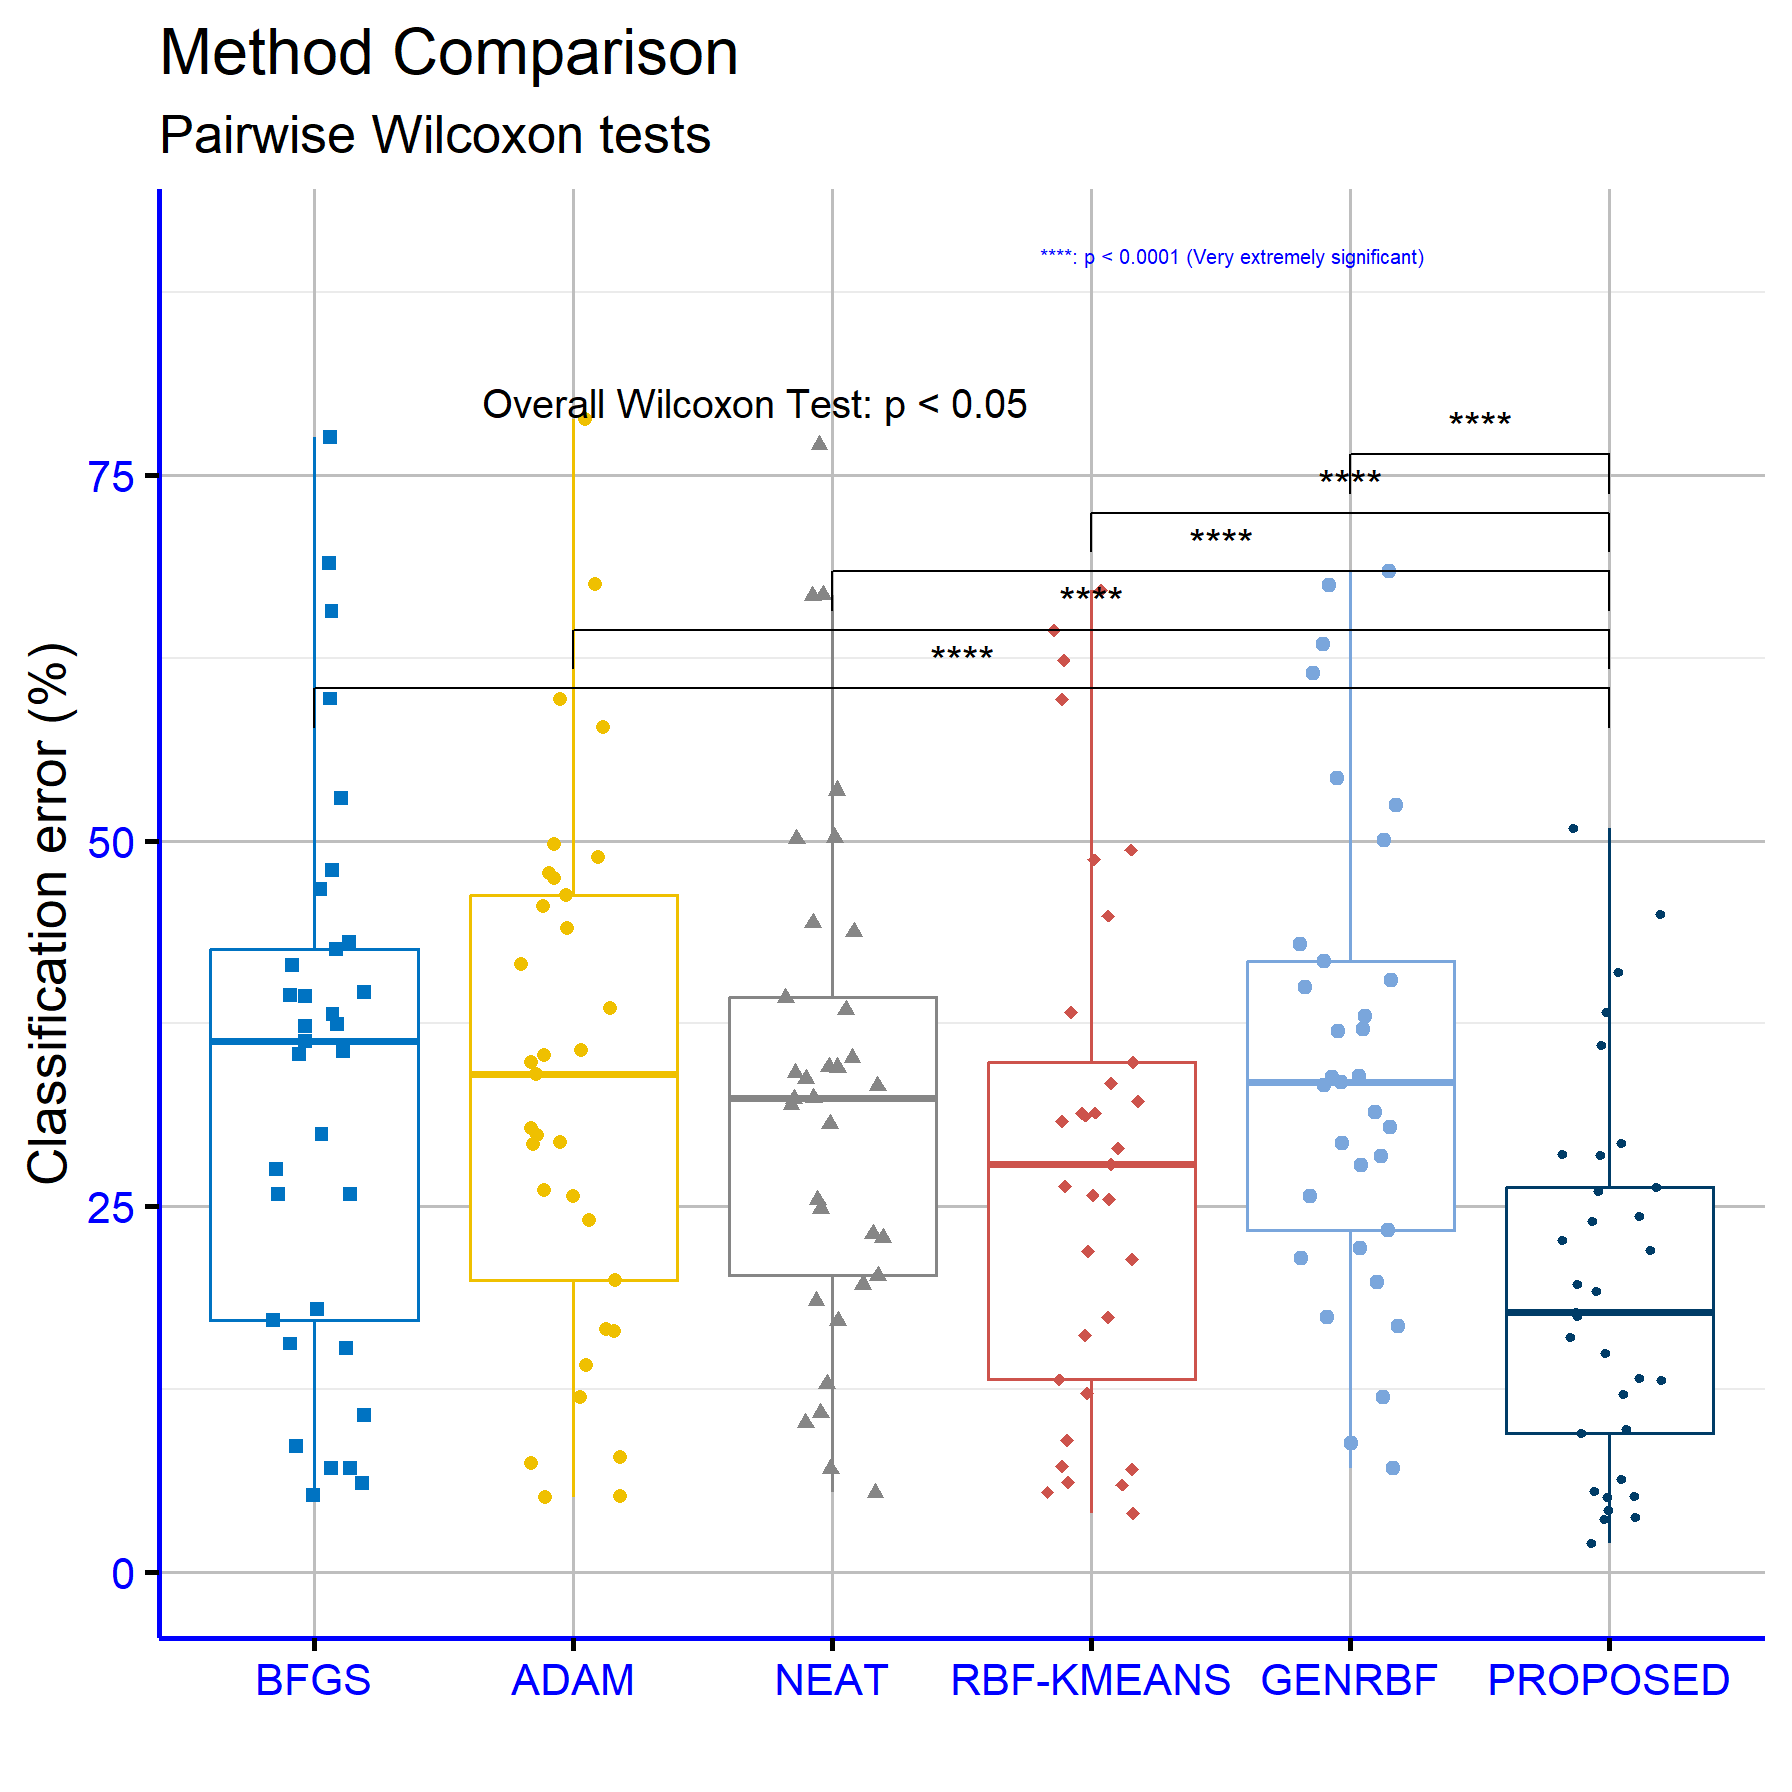
\includegraphics[scale=0.75]{stat1}

\caption{Statistical analyses of the results obtained on the classification
datasets with the machine learning methods discussed in this work.\protect\label{fig:statClass}}
\end{figure}

\begin{sidewaystable}[H]
\caption{Pairwise Wilcoxon Results: Proposed vs Baselines on classification
datasets (95\% CI \& Effect Size)\protect\label{tab:Wilcoxon1}}

\centering{}{\footnotesize{}%
\begin{tabular}{|c|c|c|c|c|c|c|c|c|}
\hline 
{\footnotesize Comparison} & {\footnotesize$n$} & {\footnotesize$V$} & {\footnotesize$r_{rank,biserial}$} & {\footnotesize$conf_{low}$} & {\footnotesize$conf_{high}$} & {\footnotesize$p$} & {\footnotesize$p_{adj}$} & {\footnotesize$p_{signif}$}\tabularnewline
\hline 
\hline 
{\footnotesize PROPOSED vs BFGS} & {\footnotesize 33} & {\footnotesize 26} & {\footnotesize -9536541889483070} & {\footnotesize -18505038146370400} & {\footnotesize -7964957107005870} & {\footnotesize 5667497792.56} & {\footnotesize 17002493377.69} & {\footnotesize{*}{*}{*}{*}}\tabularnewline
\hline 
{\footnotesize PROPOSED vs ADAM} & {\footnotesize 33} & {\footnotesize 32} & {\footnotesize -9429590017825310} & {\footnotesize -19420020785066500} & {\footnotesize -8034989453223090} & {\footnotesize 9370072082.50} & {\footnotesize 187401441650.00} & {\footnotesize{*}{*}{*}{*}}\tabularnewline
\hline 
{\footnotesize PROPOSED vs NEAT} & {\footnotesize 33} & {\footnotesize 11} & {\footnotesize -9803921568627450} & {\footnotesize -1840001089212400} & {\footnotesize -7149974070777490} & {\footnotesize 15363692460.10} & {\footnotesize 9218215476.06} & {\footnotesize{*}{*}{*}{*}}\tabularnewline
\hline 
{\footnotesize PROPOSED vs DNN} & {\footnotesize 33} & {\footnotesize 66} & {\footnotesize -8823529411764710} & {\footnotesize -8925029424575650} & {\footnotesize -3094966481225850} & {\footnotesize 1314556247229.44} & {\footnotesize 1314556247229.44} & {\footnotesize{*}{*}{*}}\tabularnewline
\hline 
{\footnotesize PROPOSED vs BAYES} & {\footnotesize 32} & {\footnotesize 17} & {\footnotesize -9678030303030300} & {\footnotesize -10224975985015600} & {\footnotesize -49000094426908900} & {\footnotesize 4040490189.97} & {\footnotesize 161619607598.76} & {\footnotesize{*}{*}{*}{*}}\tabularnewline
\hline 
{\footnotesize PROPOSED vs RBF-KMEANS} & {\footnotesize 33} & {\footnotesize 13} & {\footnotesize -9768270944741530} & {\footnotesize -12110046788330500} & {\footnotesize -4899979230676410} & {\footnotesize 18357733429.22} & {\footnotesize 9218215476.06} & {\footnotesize{*}{*}{*}{*}}\tabularnewline
\hline 
{\footnotesize PROPOSED vs GENRBF} & {\footnotesize 33} & {\footnotesize 1} & {\footnotesize -9982174688057040} & {\footnotesize -1912007131513760} & {\footnotesize -12009996230590000} & {\footnotesize 619219811.57} & {\footnotesize 4334538680.97} & {\footnotesize{*}{*}{*}{*}}\tabularnewline
\hline 
\end{tabular}}{\footnotesize\par}
\end{sidewaystable}
The Figure \ref{fig:statClass} and the Table \ref{tab:Wilcoxon1}
summarizes paired Wilcoxon signed-rank tests comparing the PROPOSED
method against each competitor on the same 33 classification datasets.
The column n is the number of paired datasets, $V$ is the Wilcoxon
signed-rank statistic, $r_{rank,biserial}$ is the rank-biserial effect
size (range -1 to 1, with more negative meaning PROPOSED has lower
error), $conf_{low}$ and $conf_{high}$ give the 95\% Hodges-Lehmann
confidence interval for the median paired difference (PROPOSED - competitor)
in percentage point error, p is the raw p-value,$p_{adj}$ is the
Holm-adjusted p-value, and $p_{signif}$ is the significance code.
Because all confidence intervals are entirely negative, the PROPOSED
method consistently shows lower error than each baseline, not just
statistical significance but a stable direction of effect across datasets.
Adjusted p-values remain very small in every comparison, from $4.33\times10^{-6}$
(vs GENRBF) up to $1.31\times10^{-4}$ (vs DNN), yielding {*}{*}{*}{*}
everywhere except the DNN comparison, which is {*}{*}{*}. Effect sizes
are uniformly large in magnitude. The strongest difference is against
GENRBF with r\ensuremath{\approx}-0.998 and a 95\% CI for the median
error reduction of roughly -19.12 to -12.01 percentage points. Very
large effects also appear versus NEAT (r\ensuremath{\approx}-0.980,
CI \ensuremath{\approx} {[}-18.40, -7.15{]}) and RBF-KMEANS (r\ensuremath{\approx}\textminus 0.977,
CI \ensuremath{\approx} {[}-12.11, -4.90{]}). Comparisons with BFGS
(r\ensuremath{\approx}-0.954, CI \ensuremath{\approx} {[}-18.51, -7.96{]})
and ADAM (r\ensuremath{\approx}-0.943, CI \ensuremath{\approx} {[}-19.42,
-8.03{]}) remain strongly favorable. The smallest, yet still large,
effect is against DNN (r\ensuremath{\approx}-0.882) with a clearly
negative CI \ensuremath{\approx} {[}-8.93, -3.09{]}. Taken together,
the results show consistent, substantial reductions in classification
error for the PROPOSED method across all baselines, with very large
effect sizes, tight negative confidence intervals, and significance
that survives multiple-comparison correction.

Table \ref{tab:Precision-and-recall} further illustrates the comparison
of precision and recall on the classification datasets between the
conventional RBF training method and the proposed technique. 

\begin{table}[H]
\begin{centering}
\begin{tabular}{|c|c|c|c|c|}
\hline 
 & \multicolumn{2}{c|}{RBF - KMEANS} & \multicolumn{2}{c|}{PROPOSED}\tabularnewline
\hline 
\hline 
DATASET & PRECISION & RECALL & PRECISION & RECALL\tabularnewline
\hline 
Alcohol & 0.507 & 0.639 & 0.723 & 0.711\tabularnewline
\hline 
Appendicitis & 0.762 & 0.875 & 0.804 & 0.722\tabularnewline
\hline 
Australian & 0.604 & 0.669 & 0.779 & 0.756\tabularnewline
\hline 
Balance & 0.753 & 0.741 & 0.794 & 0.86\tabularnewline
\hline 
Cleveland & 0.268 & 0.385 & 0.39 & 0.392\tabularnewline
\hline 
Circular & 0.941 & 0.948 & 0.963 & 0.962\tabularnewline
\hline 
Dermatology & 0.305 & 0.357 & 0.642 & 0.589\tabularnewline
\hline 
Hayes Roth & 0.34 & 0.378 & 0.68 & 0.632\tabularnewline
\hline 
Heart & 0.69 & 0.688 & 0.839 & 0.831\tabularnewline
\hline 
HeartAttack & 0.668 & 0.674 & 0.779 & 0.774\tabularnewline
\hline 
HouseVotes & 0.938 & 0.94 & 0.962 & 0.966\tabularnewline
\hline 
Ionosphere & 0.806 & 0.847 & 0.889 & 0.868\tabularnewline
\hline 
Liverdisorder & 0.665 & 0.673 & 0.689 & 0.684\tabularnewline
\hline 
Lymography & 0.688 & 0.742 & 0.783 & 0.774\tabularnewline
\hline 
Mammographic & 0.793 & 0.793 & 0.826 & 0.826\tabularnewline
\hline 
Parkinsons & 0.685 & 0.8 & 0.758 & 0.747\tabularnewline
\hline 
Pima & 0.679 & 0.732 & 0.744 & 0.705\tabularnewline
\hline 
Popfailures & 0.501 & 0.93 & 0.792 & 0.735\tabularnewline
\hline 
Regions2 & 0.331 & 0.502 & 0.645 & 0.506\tabularnewline
\hline 
Saheart & 0.607 & 0.641 & 0.669 & 0.645\tabularnewline
\hline 
Segment & 0.4 & 0.433 & 0.603 & 0.579\tabularnewline
\hline 
Sonar & 0.716 & 0.722 & 0.805 & 0.792\tabularnewline
\hline 
Spiral & 0.553 & 0.555 & 0.868 & 0.869\tabularnewline
\hline 
Statheart & 0.689 & 0.695 & 0.797 & 0.793\tabularnewline
\hline 
Student & 0.944 & 0.955 & 0.949 & 0.95\tabularnewline
\hline 
Transfusion & 0.533 & 0.641 & 0.618 & 0.534\tabularnewline
\hline 
Wdbc & 0.912 & 0.929 & 0.952 & 0.943\tabularnewline
\hline 
Wine & 0.676 & 0.763 & 0.919 & 0.907\tabularnewline
\hline 
Z\_F\_S & 0.865 & 0.871 & 0.954 & 0.96\tabularnewline
\hline 
Z\_O\_N\_F\_S & 0.534 & 0.52 & 0.621 & 0.61\tabularnewline
\hline 
ZO\_NF\_S & 0.9 & 0.9 & 0.956 & 0.6\tabularnewline
\hline 
ZONF\_S & 0.926 & 0.947 & 0.966 & 0.976\tabularnewline
\hline 
ZOO & 0.804 & 0.809 & 0.875 & 0.878\tabularnewline
\hline 
\textbf{AVERAGE} & \textbf{0.667} & \textbf{0.718} & \textbf{0.789} & \textbf{0.76}\tabularnewline
\hline 
\end{tabular}
\par\end{centering}
\caption{Comparison of precision and recall between the conventional RBF training
approach and the proposed technique.\protect\label{tab:Precision-and-recall}}
\end{table}
\begin{table}[H]
\caption{Results from the regression datasets, generated using the machine
learning methods described in this work.\protect\label{tab:expRegression}}

\centering{}{\footnotesize{}%
\begin{tabular}{|c|c|c|c|c|c|c|c|c|}
\hline 
{\footnotesize\textbf{DATASET}} & {\footnotesize\textbf{BFGS}} & {\footnotesize\textbf{ADAM}} & {\footnotesize\textbf{NEAT}} & {\footnotesize\textbf{DNN}} & {\footnotesize\textbf{BAYES}} & {\footnotesize\textbf{RBF-KMEANS}} & {\footnotesize\textbf{GENRBF}} & {\footnotesize\textbf{PROPOSED}}\tabularnewline
\hline 
{\footnotesize Abalone} & {\footnotesize 5.69} & {\footnotesize\textbf{4.30}} & {\footnotesize 9.88} & {\footnotesize 6.91} & {\footnotesize 4.81} & {\footnotesize 7.37} & {\footnotesize 9.98} & {\footnotesize 6.12}\tabularnewline
\hline 
{\footnotesize Airfoil} & {\footnotesize\textbf{0.003}} & {\footnotesize 0.005} & {\footnotesize 0.067} & {\footnotesize 0.004} & {\footnotesize 0.004} & {\footnotesize 0.27} & {\footnotesize 0.121} & {\footnotesize 0.004}\tabularnewline
\hline 
{\footnotesize Auto} & {\footnotesize 60.97} & {\footnotesize 70.84} & {\footnotesize 56.06} & {\footnotesize 13.26} & {\footnotesize 27.03} & {\footnotesize 17.87} & {\footnotesize 16.78} & {\footnotesize\textbf{8.81}}\tabularnewline
\hline 
{\footnotesize Baseball} & {\footnotesize 119.63} & {\footnotesize\textbf{77.90}} & {\footnotesize 100.39} & {\footnotesize 110.22} & {\footnotesize 88.76} & {\footnotesize 93.02} & {\footnotesize 98.91} & {\footnotesize 88.05}\tabularnewline
\hline 
{\footnotesize BK} & {\footnotesize 0.28} & {\footnotesize 0.03} & {\footnotesize 0.15} & {\footnotesize\textbf{0.02}} & {\footnotesize 0.023} & {\footnotesize 0.02} & {\footnotesize 0.023} & {\footnotesize 0.022}\tabularnewline
\hline 
{\footnotesize BL} & {\footnotesize 2.55} & {\footnotesize 0.28} & {\footnotesize 0.05} & {\footnotesize 0.006} & {\footnotesize 0.46} & {\footnotesize 0.013} & {\footnotesize 0.005} & {\footnotesize\textbf{0.0004}}\tabularnewline
\hline 
{\footnotesize Concrete} & {\footnotesize 0.066} & {\footnotesize 0.078} & {\footnotesize 0.081} & {\footnotesize 0.021} & {\footnotesize 0.013} & {\footnotesize 0.011} & {\footnotesize 0.015} & {\footnotesize\textbf{0.005}}\tabularnewline
\hline 
{\footnotesize Dee} & {\footnotesize 2.36} & {\footnotesize 0.630} & {\footnotesize 1.512} & {\footnotesize 0.31} & {\footnotesize 0.28} & {\footnotesize 0.17} & {\footnotesize 0.25} & {\footnotesize\textbf{0.15}}\tabularnewline
\hline 
{\footnotesize Housing} & {\footnotesize 97.38} & {\footnotesize 80.20} & {\footnotesize 56.49} & {\footnotesize 65.18} & {\footnotesize 57.39} & {\footnotesize 57.68} & {\footnotesize 95.69} & {\footnotesize\textbf{15.36}}\tabularnewline
\hline 
{\footnotesize Friedman} & {\footnotesize\textbf{1.26}} & {\footnotesize 22.90} & {\footnotesize 19.35} & {\footnotesize 2.75} & {\footnotesize 3.79} & {\footnotesize 7.23} & {\footnotesize 16.24} & {\footnotesize 5.99}\tabularnewline
\hline 
{\footnotesize FA} & {\footnotesize 0.426} & {\footnotesize 0.11} & {\footnotesize 0.19} & {\footnotesize 0.02} & {\footnotesize 0.051} & {\footnotesize 0.015} & {\footnotesize 0.15} & {\footnotesize\textbf{0.013}}\tabularnewline
\hline 
{\footnotesize FY} & {\footnotesize 0.22} & {\footnotesize\textbf{0.038}} & {\footnotesize 0.08} & {\footnotesize 0.039} & {\footnotesize 0.21} & {\footnotesize 0.041} & {\footnotesize 0.041} & {\footnotesize 0.054}\tabularnewline
\hline 
{\footnotesize HO} & {\footnotesize 0.62} & {\footnotesize 0.035} & {\footnotesize 0.169} & {\footnotesize 0.026} & {\footnotesize 0.034} & {\footnotesize 0.03} & {\footnotesize 0.076} & {\footnotesize\textbf{0.009}}\tabularnewline
\hline 
{\footnotesize Laser} & {\footnotesize\textbf{0.015}} & {\footnotesize 0.03} & {\footnotesize 0.084} & {\footnotesize 0.045} & {\footnotesize 0.026} & {\footnotesize 0.03} & {\footnotesize 0.075} & {\footnotesize 0.016}\tabularnewline
\hline 
{\footnotesize Mortgage} & {\footnotesize 8.23} & {\footnotesize 9.24} & {\footnotesize 14.11} & {\footnotesize 9.74} & {\footnotesize 3.01} & {\footnotesize 1.45} & {\footnotesize 1.92} & {\footnotesize\textbf{0.23}}\tabularnewline
\hline 
{\footnotesize PL} & {\footnotesize 0.29} & {\footnotesize 0.117} & {\footnotesize 0.098} & {\footnotesize 0.056} & {\footnotesize 0.056} & {\footnotesize 2.12} & {\footnotesize 0.155} & {\footnotesize\textbf{0.023}}\tabularnewline
\hline 
{\footnotesize Plastic} & {\footnotesize 20.32} & {\footnotesize 11.71} & {\footnotesize 20.77} & {\footnotesize 3.82} & {\footnotesize 3.66} & {\footnotesize 8.62} & {\footnotesize 25.91} & {\footnotesize\textbf{2.28}}\tabularnewline
\hline 
{\footnotesize PY} & {\footnotesize 0.578} & {\footnotesize 0.09} & {\footnotesize 0.075} & {\footnotesize 0.028} & {\footnotesize 0.401} & {\footnotesize\textbf{0.012}} & {\footnotesize 0.029} & {\footnotesize 0.021}\tabularnewline
\hline 
{\footnotesize Quake} & {\footnotesize 0.42} & {\footnotesize 0.06} & {\footnotesize 0.298} & {\footnotesize 0.04} & {\footnotesize 0.093} & {\footnotesize 0.07} & {\footnotesize 0.79} & {\footnotesize\textbf{0.036}}\tabularnewline
\hline 
{\footnotesize SN} & {\footnotesize 0.40} & {\footnotesize 0.026} & {\footnotesize 0.174} & {\footnotesize 0.032} & {\footnotesize 0.055} & {\footnotesize 0.027} & {\footnotesize 0.027} & {\footnotesize\textbf{0.026}}\tabularnewline
\hline 
{\footnotesize Stock} & {\footnotesize 302.43} & {\footnotesize 180.89} & {\footnotesize 12.23} & {\footnotesize 39.08} & {\footnotesize 14.43} & {\footnotesize 12.23} & {\footnotesize 25.18} & {\footnotesize\textbf{1.44}}\tabularnewline
\hline 
{\footnotesize Treasury} & {\footnotesize 9.91} & {\footnotesize 11.16} & {\footnotesize 15.52} & {\footnotesize 13.76} & {\footnotesize 3.74} & {\footnotesize 2.02} & {\footnotesize 1.89} & {\footnotesize\textbf{0.47}}\tabularnewline
\hline 
{\footnotesize\textbf{AVERAGE}} & {\footnotesize\textbf{28.82}} & {\footnotesize\textbf{21.39}} & {\footnotesize\textbf{13.99}} & {\footnotesize\textbf{11.82}} & {\footnotesize\textbf{9.18}} & {\footnotesize\textbf{9.56}} & {\footnotesize\textbf{13.38}} & {\footnotesize\textbf{5.87}}\tabularnewline
\hline 
\end{tabular}}{\footnotesize\par}
\end{table}

Table \ref{tab:expRegression} evaluates the performance of eight
regression methods on twenty-one datasets using absolute errors. The
average error shows a clear overall advantage for the proposed method
at 5.87, followed by BAYES at 9.18, RBF-KMEANS at 9.56, DNN at 11.82,
NEAT at 13.99, GENRBF at 13.38, ADAM at 21.39, and BFGS at 28.82.
Relative to the best competing average, BAYES, the proposed method
reduces error by about 3.31 points (\ensuremath{\approx}36\%). The
reduction versus RBF-KMEANS is about 3.69 points (\ensuremath{\approx}39\%),
versus DNN about 5.95 points (\ensuremath{\approx}50\%), and relative
to NEAT and GENRBF the drops are roughly 58\% and 56\%, respectively.
The advantage is even larger against ADAM and BFGS, where the mean
error is nearly halved or more.

Across individual datasets, the proposed method attains the best value
in roughly two thirds of the cases. It is clearly first on Auto, BL,
Concrete, Dee, Housing, FA, HO, Mortgage, PL, Plastic, Quake, Stock,
and Treasury, with particularly large margins on Housing and Stock
where errors fall to 15.36 and 1.44 while other methods range from
tens to hundreds. On Airfoil it is essentially tied with the best
at 0.004, while BFGS is slightly lower at 0.003. There are datasets
where other methods lead, such as Abalone where ADAM and BAYES are
ahead; Friedman and Laser where BFGS gives the best value; BK where
DNN and RBF-KMEANS lead; and PY where RBF-KMEANS is lower. Despite
these isolated exceptions, the proposed method remains consistently
among the top performers and most often the best.

Overall, the proposed approach combines a very low average error with
broad superiority across diverse problem types and error scales, from
thousandths to very large magnitudes. The consistency of the gains
and the size of the margins over all baselines indicate it is the
most efficient and generalizable choice among the regression methods
considered.

\begin{figure}[H]
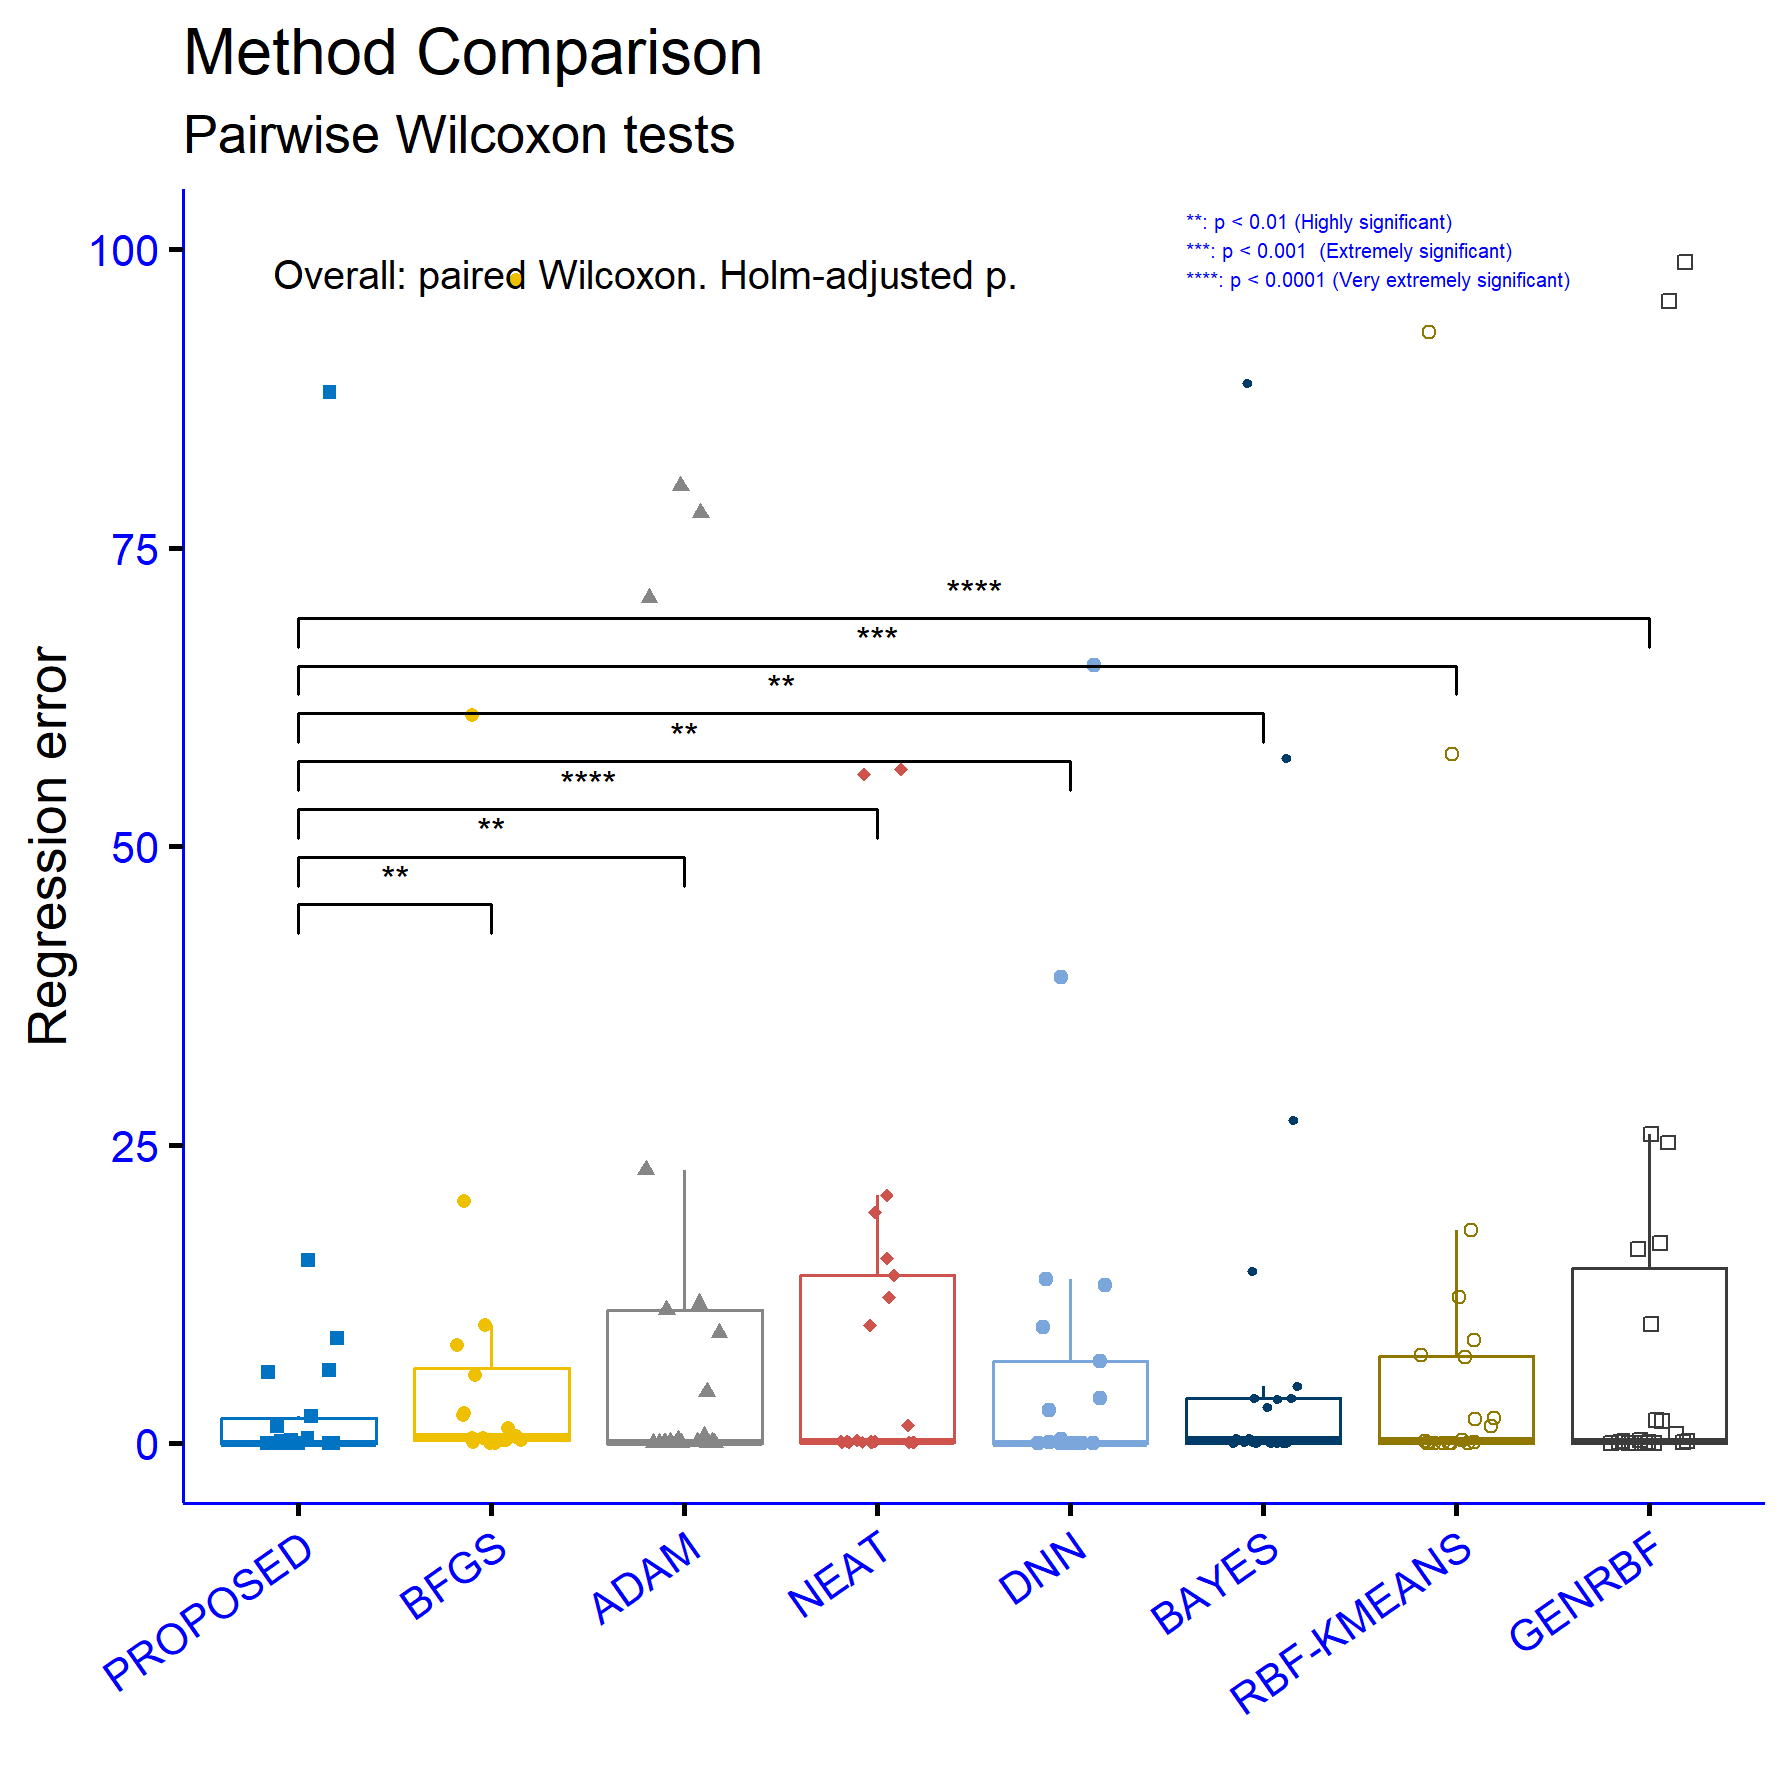
\includegraphics[scale=0.75]{stat2}

\caption{Statistical analysis comparing the results produced by the set of
machine learning methods applied to the regression datasets.\protect\label{fig:statRegression}}
\end{figure}

\begin{sidewaystable}[H]
\caption{Pairwise Wilcoxon Results: Proposed vs Baselines on regression datasets
(95\% CI \& Effect Size)\protect\label{tab:Wilcoxon2}}

\centering{}{\scriptsize{}%
\begin{tabular}{|c|c|c|c|c|c|c|c|c|}
\hline 
{\scriptsize Comparison} & {\scriptsize$n$} & {\scriptsize$V$} & {\scriptsize$r_{rank,biserial}$} & {\scriptsize$conf_{low}$} & {\scriptsize$conf_{high}$} & {\scriptsize$p$} & {\scriptsize$p_{adj}$} & {\scriptsize$p_{signif}$}\tabularnewline
\hline 
\hline 
{\scriptsize PROPOSED vs BFGS} & {\scriptsize 22.00} & {\scriptsize 28.00} & {\scriptsize -8893280632411070} & {\scriptsize -20509998654975500} & {\scriptsize -31607290631815900.0} & {\scriptsize 14644689859755000.00} & {\scriptsize 5541059559701440.00} & {\scriptsize{*}{*}}\tabularnewline
\hline 
{\scriptsize PROPOSED vs ADAM} & {\scriptsize 21.00} & {\scriptsize 33.00} & {\scriptsize -8571428571428570} & {\scriptsize -2734490876933390} & {\scriptsize -41569559046521200.0} & {\scriptsize 4370173456024450.00} & {\scriptsize 6265548255802160.00} & {\scriptsize{*}{*}}\tabularnewline
\hline 
{\scriptsize PROPOSED vs NEAT} & {\scriptsize 22.00} & {\scriptsize 0.00} & {\scriptsize -1} & {\scriptsize -9925969319615250} & {\scriptsize -16000237429855300.0} & {\scriptsize 43012521191.44} & {\scriptsize 3010876483400.92} & {\scriptsize{*}{*}{*}}\tabularnewline
\hline 
{\scriptsize PROPOSED vs DNN} & {\scriptsize 21.00} & {\scriptsize 23.00} & {\scriptsize -9004329004329000} & {\scriptsize -11086980158184000} & {\scriptsize -12031295944894700.0} & {\scriptsize 13852648899253600.00} & {\scriptsize 5541059559701440.00} & {\scriptsize{*}{*}}\tabularnewline
\hline 
{\scriptsize PROPOSED vs BAYES} & {\scriptsize 21.00} & {\scriptsize 30.00} & {\scriptsize -8701298701298700} & {\scriptsize -5839992445666000} & {\scriptsize -33511395308536000.0} & {\scriptsize 31327741279010800.00} & {\scriptsize 6265548255802160.00} & {\scriptsize{*}{*}}\tabularnewline
\hline 
{\scriptsize PROPOSED vs RBF-KMEANS} & {\scriptsize 22.00} & {\scriptsize 14.00} & {\scriptsize -9446640316205530} & {\scriptsize -4523464832268890} & {\scriptsize -3407835793499720.0} & {\scriptsize 276740186614.05} & {\scriptsize 13837009330702700.00} & {\scriptsize{*}{*}}\tabularnewline
\hline 
{\scriptsize PROPOSED vs GENRBF} & {\scriptsize 22.00} & {\scriptsize 6.00} & {\scriptsize -9762845849802370} & {\scriptsize -10249984407899800} & {\scriptsize -9806889388206810.0} & {\scriptsize 9774004411.05} & {\scriptsize 586440264662.75} & {\scriptsize{*}{*}{*}}\tabularnewline
\hline 
\end{tabular}}{\scriptsize\par}
\end{sidewaystable}

The Figure \ref{fig:statRegression} and the Table \ref{tab:Wilcoxon2}
summarizes paired Wilcoxon signed-rank tests between PROPOSED and
each method on the same regression datasets. In every comparison the
95\% confidence interval is entirely negative, so PROPOSED consistently
attains lower error than each baseline. Holm-adjusted p-values range
from about $5.86\times10^{-4}$ to 0.0063, yielding {*}{*} or {*}{*}{*}
across all pairings, indicating strong though not extreme significance.
Effect sizes are very large in absolute value, implying a consistent
sign of the differences across datasets. The strongest dominance is
against NEAT with r\ensuremath{\approx}-1 and V=0, meaning that in
every non-tied pair PROPOSED was better, with a confidence interval
roughly {[}-9.93, -0.16{]}. Similarly large effects appear against
GENRBF (r\ensuremath{\approx}-0.976, CI {[}-10.25, -0.098{]}) and
RBF-KMEANS (r\ensuremath{\approx}-0.945, CI {[}-4.52, -0.034{]}),
the upper bound near zero indicates that the typical improvement can
range from very small to several points depending on the dataset.
Against BFGS and ADAM the effects remain very large (r\ensuremath{\approx}-0.889
and r\ensuremath{\approx}-0.857, respectively) with wider intervals
{[}-20.51, -0.316{]} and {[}-27.34, -0.0416{]}, showing substantial
heterogeneity in the magnitude of error reduction while the direction
remains in favor of PROPOSED. The most challenging comparison is with
DNN: although \textbar r\textbar{} is still very large (\ensuremath{\approx}0.900),
the CI is narrow and close to zero {[}-11.09, -0.012{]}, implying
that while superiority is consistent, the typical error reduction
may be small in many cases.

Overall, the results demonstrate that PROPOSED systematically outperforms
all alternatives on regression, with very large rank-based effect
sizes, negative and robust confidence intervals, and significance
that survives multiple-comparison correction. The strength of the
improvement varies by problem and is more modest against DNN, but
the direction of the effect is consistently in favor of PROPOSED across
all comparisons.

\subsection{Experiments with different values of scale factor $F$ }

In order to evaluate the stability and reliability of the current
work when its critical parameters are altered, a series of additional
experiments were executed. In one of them, the stability of the technique
was studied with the change of the scale factor $F$.\textbf{ }This
factor regulates the range of network parameter values and is scaled
as a multiple of the initial estimates obtained from the first-phase
K-Means method.\textbf{ }In this series of experiments, the value
of $F$ was altered in the range $[1,8]$. 

The effect of the scale factor $F$ on the performance of the proposed
machine learning model is presented in Table \ref{tab:expClass}.
The parameter $F$ takes four different values, 1, 2, 4, and 8, and
for each dataset the classification error rate is reported. Analyzing
the mean values, it is observed that $F=2$ and $F=4$ achieve the
best overall performance, with average errors of 19.45\% and 18.53\%
respectively, compared to 20.99\% for $F=1$ and 18.60\% for $F=8$.
This indicates that selecting an intermediate value of the initialization
factor improves performance, reducing the error by about two percentage
points relative to the baseline case of $F=1$. At the individual
dataset level, interesting patterns emerge. For example, in Sonar
the error drops significantly from 32.90\% at $F=1$ to 18.75\% at
$F=4$, suggesting that the parameter $F$ strongly influences performance
in certain problems. In contrast, in Spiral increasing $F$ worsens
the results, as the error rises from 12.03\% at $F=1$ to 23.56\%
at $F=8$. Similarly, in the Australian dataset a gradual increase
of $F$ from 1 to 8 systematically improves performance, reducing
the error from 24.04\% to 20.59\%. Overall, the data show that the
effect of the scale factor is not uniform across all problems, but
the general trend indicates improvement when $F$ increases from 1
to 2 or 4. Choosing $F=4$ appears to yield the best mean result,
although the difference compared with $F=8$ is very small. Therefore,
it can be concluded that tuning this parameter plays an important
role in the stability and accuracy of the model, and that intermediate
values such as 4 constitute a good general choice.

\begin{table}[H]
\caption{Results of applying the proposed method to the classification datasets,
with the critical parameter $F$ ranging between 1 and 8.\protect\label{tab:expClassF}}

\centering{}%
\begin{tabular}{|c|c|c|c|c|}
\hline 
\textbf{DATASET} & $F=1$ & \textbf{$F=2$} & $F=4$ & $F=8$\tabularnewline
\hline 
\hline 
Alcohol & 28.83\% & \textbf{28.57\%} & 28.83\% & 30.09\%\tabularnewline
\hline 
Appendicitis & 14.60\% & 15.00\% & \textbf{14.40\%} & 15.50\%\tabularnewline
\hline 
Australian & 24.04\% & 22.67\% & 21.52\% & \textbf{20.59\%}\tabularnewline
\hline 
Balance & 21.03\% & 13.11\% & 11.87\% & \textbf{11.44\%}\tabularnewline
\hline 
Cleveland & \textbf{50.45\%} & 50.86\% & 51.59\% & 50.90\%\tabularnewline
\hline 
Circular & 4.13\% & 5.13\% & 3.67\% & \textbf{3.49\%}\tabularnewline
\hline 
Dermatology & 38.34\% & 36.00\% & 35.83\% & \textbf{34.97\%}\tabularnewline
\hline 
Hayes Roth & 51.85\% & 38.31\% & \textbf{32.62\%} & 33.92\%\tabularnewline
\hline 
Heart & 17.26\% & 16.07\% & 15.63\% & \textbf{15.30\%}\tabularnewline
\hline 
HeartAttack & 22.07\% & 19.20\% & 19.30\% & \textbf{19.07\%}\tabularnewline
\hline 
HouseVotes & 4.13\% & 3.65\% & \textbf{3.39\%} & 4.81\%\tabularnewline
\hline 
Ionosphere & 14.69\% & 12.17\% & 8.83\% & \textbf{7.51\%}\tabularnewline
\hline 
Liverdisorder & 29.35\% & 29.29\% & \textbf{28.53\%} & 29.23\%\tabularnewline
\hline 
Lymography & 26.86\% & 24.36\% & \textbf{18.07\%} & 19.86\%\tabularnewline
\hline 
Mammographic & 18.21\% & 17.79\% & \textbf{16.75\%} & 17.05\%\tabularnewline
\hline 
Parkinsons & 18.32\% & 17.53\% & 15.68\% & \textbf{14.05\%}\tabularnewline
\hline 
Pima & 23.53\% & 24.02\% & 23.72\% & \textbf{23.26\%}\tabularnewline
\hline 
Popfailures & 7.83\% & 6.33\% & 5.15\% & \textbf{4.69\%}\tabularnewline
\hline 
Regions2 & 26.27\% & 26.29\% & 26.15\% & \textbf{25.73\%}\tabularnewline
\hline 
Saheart & 29.24\% & \textbf{28.50\%} & 28.74\% & 29.41\%\tabularnewline
\hline 
Segment & 45.08\% & 45.00\% & 42.14\% & \textbf{42.10\%}\tabularnewline
\hline 
Sonar & 32.90\% & 22.00\% & 18.75\% & \textbf{18.05\%}\tabularnewline
\hline 
Spiral & \textbf{12.03\%} & 13.26\% & 16.66\% & 23.56\%\tabularnewline
\hline 
Statheart & \textbf{19.30\%} & 19.67\% & 20.00\% & 19.44\%\tabularnewline
\hline 
Student & 6.33\% & 5.23\% & \textbf{5.10\%} & 5.55\%\tabularnewline
\hline 
Transfusion & 25.54\% & 26.04\% & 25.66\% & \textbf{24.42\%}\tabularnewline
\hline 
Wdbc & \textbf{4.86\%} & 5.54\% & 5.75\% & 5.29\%\tabularnewline
\hline 
Wine & 12.18\% & 9.47\% & 8.59\% & \textbf{7.65\%}\tabularnewline
\hline 
Z\_F\_S & 4.37\% & 3.73\% & 3.73\% & \textbf{3.37\%}\tabularnewline
\hline 
Z\_O\_N\_F\_S & \textbf{39.80\%} & 41.00\% & 40.04\% & 40.80\%\tabularnewline
\hline 
ZO\_NF\_S & 4.26\% & 4.24\% & 4.58\% & \textbf{3.78\%}\tabularnewline
\hline 
ZONF\_S & 2.52\% & 1.98\% & 2.58\% & \textbf{1.96\%}\tabularnewline
\hline 
ZOO & 12.40\% & 9.80\% & 7.60\% & \textbf{6.90\%}\tabularnewline
\hline 
\textbf{AVERAGE} & \textbf{20.99\%} & \textbf{19.45\%} & \textbf{18.53\%} & \textbf{18.60\%}\tabularnewline
\hline 
\end{tabular}
\end{table}
Table \ref{tab:expRegressionF} shows the effect of the scale factor
$F$ on the performance of the proposed regression model. Based on
the mean errors, the best overall performance occurs at $F=4$ with
an average error of 5.68, while the values for $F=1,F=2$ and $F=8$
are 5.94, 5.87, and 5.78, respectively. The differences across the
four settings are not large, but they indicate that intermediate values
and especially $F=4$ tend to offer the best accuracy stability trade-off.
At the level of individual datasets, substantial variations are observed.
For Friedman the reduction is dramatic, with error dropping from 6.74
at $F=1$ to 1.41 at $F=8$, highlighting that proper tuning of $F$
can have a strong impact on performance. Laser shows a similarly large
improvement, from 0.027 at $F=1$ to just 0.0024 at $F=8$. Mortgage
also improves markedly, from $0.67$ at $F=1$ to 0.015 at $F=8$.
By contrast, in some datasets the value of $F$ has little practical
effect, such as Quake and HO, where errors remain nearly constant
regardless of F. There are also cases like Housing where increasing
$F$ degrades performance, with error rising from 14.64 at $F=1$
to 18.48 at $F=8$. Overall, the results indicate that the scale factor
$F$ has a significant but nonuniform influence on model performance.
In some datasets it sharply reduces error, while in others its impact
is negligible or even negative. Nevertheless, the aggregate picture
based on the mean errors suggests that $F=4$ and $F=8$ yield the
most reliable results, with $F=4$ being the preferred choice for
a general-purpose setting.
\begin{table}[H]
\caption{Results of applying the proposed method to the regression datasets,
with the critical parameter $F$ ranging between 1 and 8.\protect\label{tab:expRegressionF}}

\centering{}%
\begin{tabular}{|c|c|c|c|c|}
\hline 
\textbf{DATASET} & $F=1$ & \textbf{$F=2$} & $F=4$ & $F=8$\tabularnewline
\hline 
Abalone & 6.70 & 6.12 & 5.70 & \textbf{5.56}\tabularnewline
\hline 
Airfoil & \textbf{0.004} & 0.004 & 0.004 & 0.004\tabularnewline
\hline 
Auto & 10.04 & \textbf{8.81} & 9.82 & 10.92\tabularnewline
\hline 
Baseball & 87.01 & 88.05 & \textbf{85.87} & 86.76\tabularnewline
\hline 
BK & 0.023 & 0.022 & 0.024 & \textbf{0.02}\tabularnewline
\hline 
BL & 0.01 & 0.0004 & 0.0002 & \textbf{0.00007}\tabularnewline
\hline 
Concrete & 0.008 & \textbf{0.005} & 0.005 & 0.006\tabularnewline
\hline 
Dee & \textbf{0.15} & 0.15 & 0.16 & 0.16\tabularnewline
\hline 
Housing & \textbf{14.64} & 15.36 & 17.34 & 18.48\tabularnewline
\hline 
Friedman & 6.74 & 5.99 & 2.06 & \textbf{1.41}\tabularnewline
\hline 
FA & \textbf{0.012} & 0.013 & 0.012 & 0.013\tabularnewline
\hline 
FY & 0.055 & 0.054 & 0.054 & \textbf{0.053}\tabularnewline
\hline 
HO & \textbf{0.009} & 0.009 & 0.01 & 0.009\tabularnewline
\hline 
Laser & 0.027 & 0.016 & 0.005 & \textbf{0.0024}\tabularnewline
\hline 
Mortgage & 0.67 & 0.23 & 0.035 & \textbf{0.015}\tabularnewline
\hline 
PL & 0.023 & 0.023 & 0.023 & \textbf{0.022}\tabularnewline
\hline 
Plastic & 2.32 & 2.28 & 2.26 & \textbf{2.22}\tabularnewline
\hline 
PY & 0.019 & 0.021 & 0.013 & \textbf{0.011}\tabularnewline
\hline 
Quake & \textbf{0.036} & 0.036 & 0.036 & 0.036\tabularnewline
\hline 
SN & \textbf{0.024} & 0.026 & 0.025 & 0.024\tabularnewline
\hline 
Stock & 1.69 & \textbf{1.44} & 1.49 & 1.48\tabularnewline
\hline 
Treasury & 0.57 & 0.47 & 0.035 & \textbf{0.031}\tabularnewline
\hline 
\textbf{AVERAGE} & \textbf{5.94} & \textbf{5.87} & \textbf{5.68} & \textbf{5.78}\tabularnewline
\hline 
\end{tabular}
\end{table}

The significance levels for comparisons among different values of
the parameter $F$ in the proposed machine learning method, using
the classification datasets, are shown in Figure \ref{fig:statClassF}.
The analysis shows that the comparison between $F=1$ and $F=2$ results
in high statistical significance with $p<0.01$, indicating that the
transition from the initial value to $F=2$ has a substantial impact
on performance. Similarly, the comparison between $F=2$ and $F=4$
also shows high statistical significance with $p<0.01$, suggesting
that further increasing the parameter continues to positively affect
the results. However, the comparison between $F=4$ and $F=8$ is
characterized as not statistically significant, since $p>0.05$, which
means that increasing the parameter beyond $F=4$ does not bring a
meaningful difference in performance. Overall, the findings indicate
that smaller values of $F$ play a critical role in improving the
model, while increases beyond 4 do not lead to further statistically
significant improvements.

\begin{figure}[H]
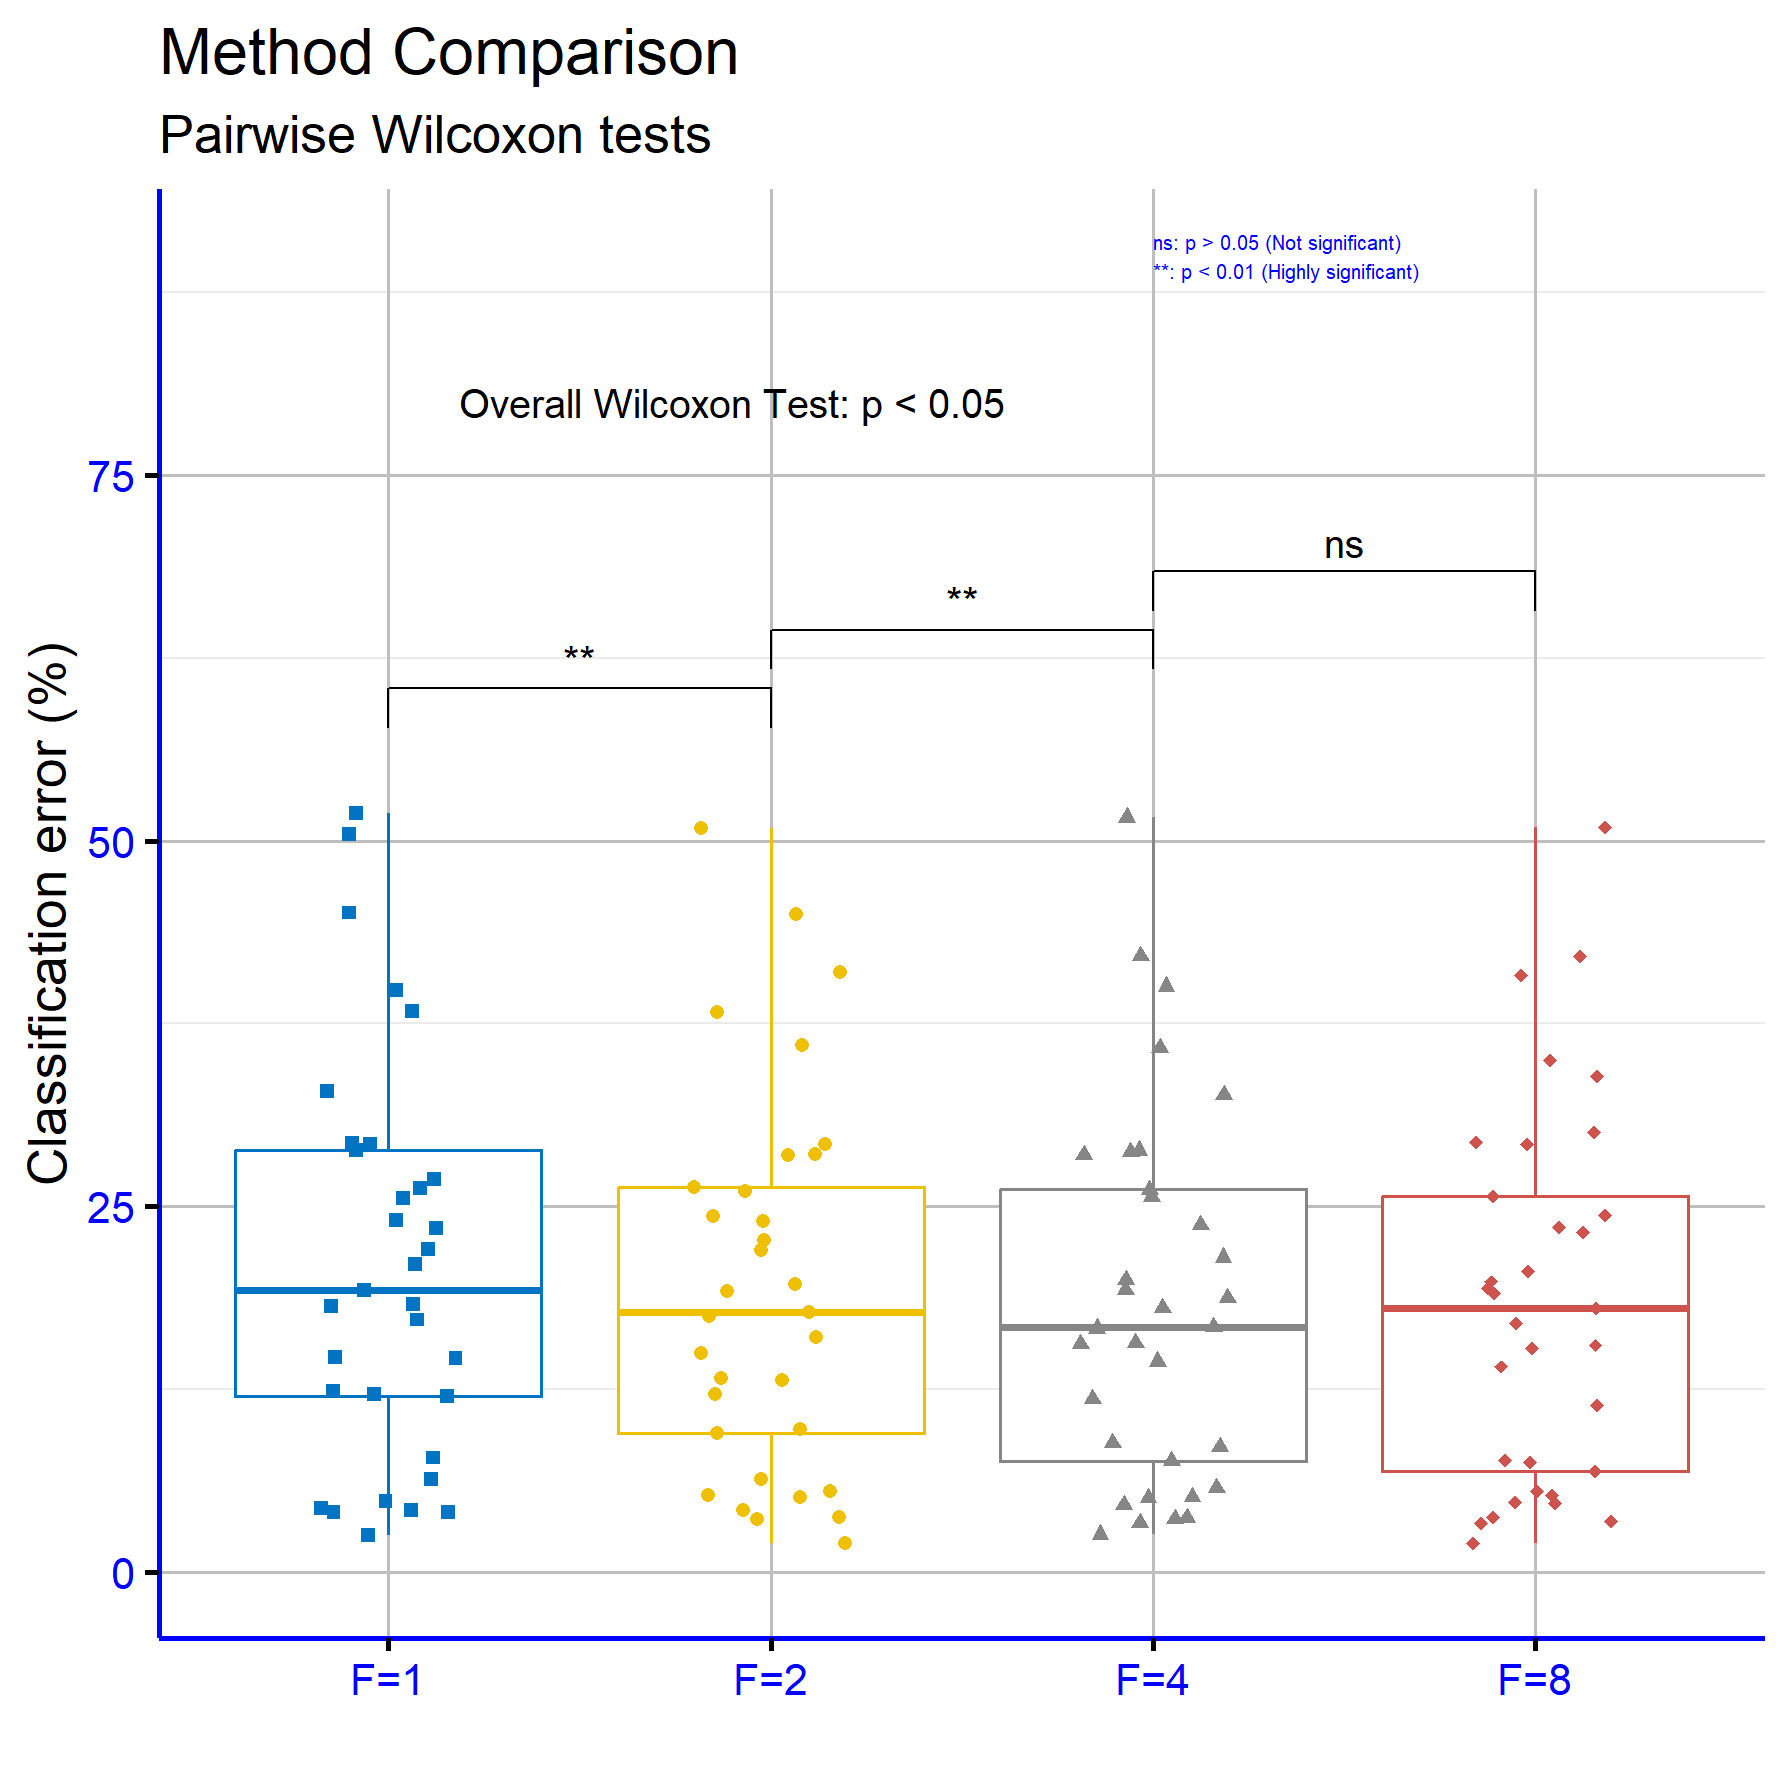
\includegraphics[scale=0.75]{stat3}

\caption{Statistical evaluation of the outcomes produced by the proposed approach
on the classification datasets, considering variations in the parameter
$F$. \protect\label{fig:statClassF}}

\end{figure}
The significance levels for comparisons among different values of
the parameter $F$ in the proposed method, using the regression datasets,
are presented in \ref{fig:statRegressionF}. The results show that
none of the comparisons $F=1$ vs $F=2$, $F=2$ vs $F=4$, and $F=4$
vs $F=8$ exhibit statistically significant differences, since in
all cases $p>0.05$. These results suggest that variations in the
parameter $F$ do not significantly influence the performance of the
model on regression tasks. Therefore, it can be concluded that the
choice of the $F$ value is not of critical importance for these datasets
and that the model remains stable regardless of the specific setting
of this parameter.
\begin{figure}[H]
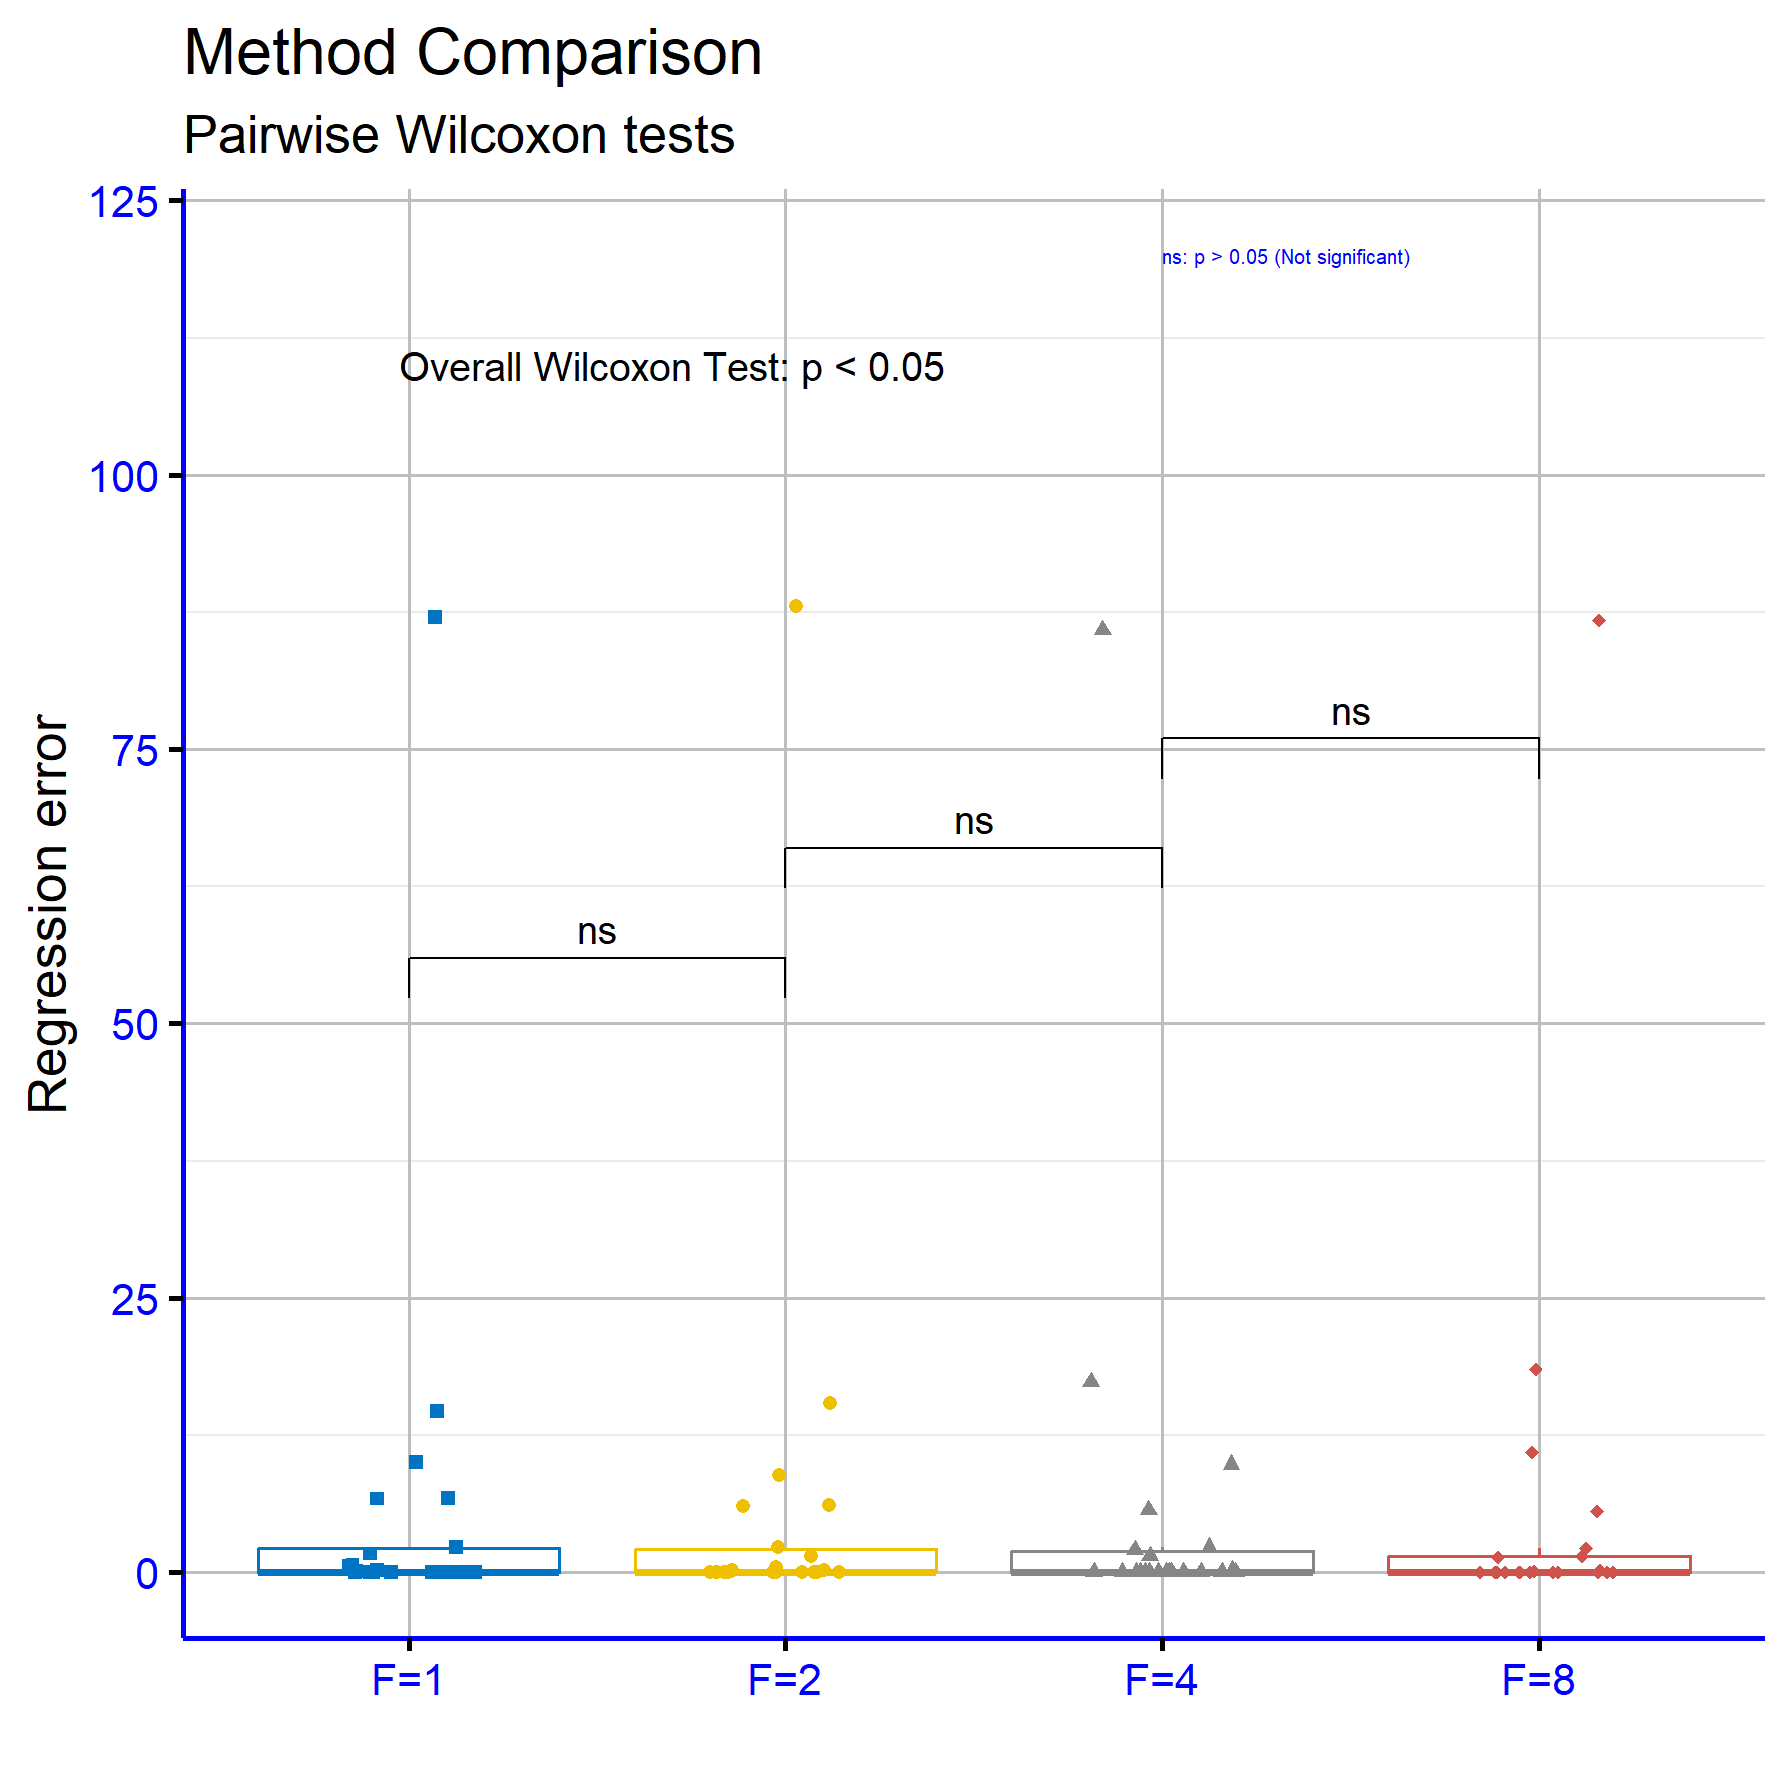
\includegraphics[scale=0.75]{stat4}

\caption{Statistical evaluation of the outcomes produced by the proposed approach
on the regression datasets, with variations in the parameter $F$.\protect\label{fig:statRegressionF}}
\end{figure}


\subsection{Experiments with differential initialization methods for variances}

The stability of the proposed method was also evaluated by employing
a different procedure to determine the range of $\sigma$ parameters
for the radial functions.\textbf{ }Here, the $\sigma$ parameters
were initially estimated using the variance calculated by the K-Means
algorithm.\textbf{ }This calculation scheme is denoted as $\sigma_{1}$
in the following experimental tables. In this additional set of experiments,
two more techniques were used, which will be denoted as $\sigma_{\mbox{avg}}$
and $\sigma_{\mbox{max}}$ in the following tables. In the $\sigma_{\mbox{avg}}$
the following calculation is performed:
\begin{equation}
\sigma_{\mbox{avg}}=\frac{1}{k}\sum_{i=1}^{k}\sigma_{i}\label{eq:sigma_avg}
\end{equation}
Subsequently $\sigma_{\mbox{avg}}$ is used to determine the range
of values of the $\sigma$ parameters of the radial functions of the
network. In the $\sigma_{\mbox{avg}}$ the following quantity is calculated:
\begin{equation}
\sigma_{\mbox{max}}=\max\sigma_{i}\label{eq:sigma_max}
\end{equation}
This quantity is then employed to define the range of $\sigma$ parameter
values for the radial functions. Table \ref{tab:expClassSigma} presents
the effect of three different calculation techniques for the $\sigma$
parameters used in the radial basis functions of the RBF model. The
techniques are a fixed value $\sigma_{1}$, the mean distance-based
initialization $\left(\sigma_{\mbox{avg}}\right)$, and the maximum
distance--based initialization $\left(\sigma_{\mbox{max}}\right)$.
Based on the mean errors, the maximum-distance technique yields the
lowest overall error at 19.18\%. Very close is the mean-distance technique
at 19.27\%, while the simple $\sigma_{1}$ initialization has a slightly
higher error of 19.45\%. Although the differences among the three
approaches are small, the two adaptive methods $\left(\sigma_{\mbox{avg}}\ \mbox{and}\ \sigma_{\mbox{max}}\right)$
tend to produce marginally better overall performance. At the individual
dataset level, behaviors vary. For example, on Wine the $\sigma_{\mbox{max}}$
choice reduces error to 7.06\%, far below the 9.47\% obtained with
$\sigma_{1}$. On Dermatology, $\sigma_{1}$ performs better than
the other two, whereas on Segment the mean-based option is preferable.
In some cases the differences are minor e.g., Circular, Pima, and
Popfailures where all techniques are comparable; in others the choice
of technique materially affects performance, as in Transfusion, where
error drops from 26.04\% with $\sigma_{1}$ to about 22.78\% with
the other two methods. Overall, the statistical picture indicates
that no single technique dominates across all datasets. Nevertheless,
methods that adapt $\sigma$ to the geometry of the data $\left(\sigma_{\mbox{avg}}\ \mbox{and}\ \sigma_{\mbox{max}}\right)$
tend to yield more reliable and stable results, while the fixed value
lags slightly. The average differences are modest, but for certain
problems the choice can significantly impact final performance.

\begin{table}[H]
\caption{The proposed method was evaluated on the classification datasets using
various approaches to compute the $\sigma$ parameters in the radial
basis functions. \protect\label{tab:expClassSigma}}

\centering{}%
\begin{tabular}{|c|c|c|c|}
\hline 
\textbf{DATASET} & \textbf{$\sigma_{1}$} & $\sigma_{\mbox{avg}}$ & $\sigma_{\mbox{max}}$\tabularnewline
\hline 
\hline 
Alcohol & 28.57\% & 28.47\% & \textbf{26.17\%}\tabularnewline
\hline 
Appendicitis & 15.00\% & \textbf{14.20\%} & 15.70\%\tabularnewline
\hline 
Australian & \textbf{22.67\%} & 25.14\% & 29.96\%\tabularnewline
\hline 
Balance & 13.11\% & 12.92\% & \textbf{12.23\%}\tabularnewline
\hline 
Cleveland & \textbf{50.86\%} & 51.76\% & 51.24\%\tabularnewline
\hline 
Circular & 5.13\% & 4.78\% & \textbf{4.45\%}\tabularnewline
\hline 
Dermatology & \textbf{36.00\%} & 37.54\% & 37.09\%\tabularnewline
\hline 
Hayes Roth & 38.31\% & 38.00\% & \textbf{35.69\%}\tabularnewline
\hline 
Heart & 16.07\% & 16.52\% & \textbf{15.41\%}\tabularnewline
\hline 
HeartAttack & 19.20\% & 19.70\% & \textbf{18.97\%}\tabularnewline
\hline 
HouseVotes & 3.65\% & 3.31\% & \textbf{3.22\%}\tabularnewline
\hline 
Ionosphere & \textbf{12.17\%} & 13.00\% & 12.83\%\tabularnewline
\hline 
Liverdisorder & 29.29\% & 28.38\% & \textbf{27.77\%}\tabularnewline
\hline 
Lymography & 24.36\% & \textbf{22.43\%} & 23.50\%\tabularnewline
\hline 
Mammographic & 17.79\% & \textbf{17.28\%} & 17.41\%\tabularnewline
\hline 
Parkinsons & 17.53\% & \textbf{14.74\%} & 14.89\%\tabularnewline
\hline 
Pima & 24.02\% & \textbf{23.28\%} & 23.91\%\tabularnewline
\hline 
Popfailures & 6.33\% & 6.37\% & \textbf{6.24\%}\tabularnewline
\hline 
Regions2 & 26.29\% & \textbf{25.47\%} & 25.61\%\tabularnewline
\hline 
Saheart & 28.50\% & 28.89\% & \textbf{28.28\%}\tabularnewline
\hline 
Segment & 45.00\% & \textbf{43.65\%} & 46.36\%\tabularnewline
\hline 
Sonar & 22.00\% & 21.90\% & \textbf{21.30\%}\tabularnewline
\hline 
Spiral & \textbf{13.26\%} & 13.73\% & 13.37\%\tabularnewline
\hline 
Statheart & 19.67\% & 20.15\% & \textbf{19.00\%}\tabularnewline
\hline 
Student & \textbf{5.23\%} & 5.58\% & 5.23\%\tabularnewline
\hline 
Transfusion & 26.04\% & \textbf{22.78\%} & 22.79\%\tabularnewline
\hline 
Wdbc & 5.54\% & 5.22\% & \textbf{5.21\%}\tabularnewline
\hline 
Wine & 9.47\% & 7.93\% & 7.06\%\tabularnewline
\hline 
Z\_F\_S & 3.73\% & \textbf{3.70\%} & 3.73\%\tabularnewline
\hline 
Z\_O\_N\_F\_S & 41.00\% & \textbf{40.20\%} & 41.12\%\tabularnewline
\hline 
ZO\_NF\_S & \textbf{4.24\%} & 4.42\% & 4.84\%\tabularnewline
\hline 
ZONF\_S & 1.98\% & \textbf{1.92\%} & 2.06\%\tabularnewline
\hline 
ZOO & \textbf{9.80\%} & 12.50\% & 10.30\%\tabularnewline
\hline 
\textbf{AVERAGE} & \textbf{19.45\%} & \textbf{19.27\%} & \textbf{19.18\%}\tabularnewline
\hline 
\end{tabular}
\end{table}
Table \ref{tab:expRegressionSigma} presents the effect of three different
calculation techniques for the $\sigma$ parameters used in the radial
basis functions of RBF model. Based on the mean errors, the distance--average
method yields the lowest overall error at 5.81. Very close is the
fixed value $\sigma_{1}$ with a mean error of 5.87, while the maximum-distance
method shows a slightly higher mean error of 5.96. The difference
among the three methods is small, indicating that all can deliver
comparable performance at a general level, with a slight advantage
for the distance--average approach. At the level of individual datasets,
however, significant variations are observed. For example, in Mortgage
the $\sigma_{\mbox{max}}$ method reduces the error dramatically from
0.23 with $\sigma_{1}$ to 0.021, while $\sigma_{\mbox{avg}}$ also
provides a much better result with 0.041. In Treasury the improvement
is again substantial, as the error decreases from 0.47 with $\sigma_{1}$
to just 0.08 using $\sigma_{\mbox{max}}$. In Stock the reduction
is clear, from 1.44 to 1.23, while in Plastic both $\sigma_{\mbox{avg}}$
and $\sigma_{\mbox{max}}$ yield lower errors than $\sigma_{1}$.
On the other hand, in datasets such as Housing, the use of $\sigma_{\mbox{max}}$
worsens performance, increasing the error from 15.36 with $\sigma_{1}$
to 19.45. Similarly, in Auto and Baseball the lowest errors are obtained
with $\sigma_{1}$, whereas the alternative techniques result in slightly
worse performance. Overall, the results show that the choice of calculation
technique for $\sigma$ can significantly affect performance in certain
problems, while in others the difference is negligible. Although no
method consistently outperforms the others across all datasets, the
distance--average method appears slightly more reliable overall,
while the maximum-distance method can in some cases produce very large
improvements but in others lead to a degradation of performance.

\begin{table}[H]
\caption{The proposed method was applied to the regression datasets, and results
were analyzed using various approaches to compute the $\sigma$ parameters
of the radial functions.\protect\label{tab:expRegressionSigma}}

\centering{}%
\begin{tabular}{|c|c|c|c|}
\hline 
\textbf{DATASET} & \textbf{$\sigma_{1}$} & $\sigma_{\mbox{avg}}$ & $\sigma_{\mbox{max}}$\tabularnewline
\hline 
Abalone & 6.12 & 6.06 & 5.43\tabularnewline
\hline 
Airfoil & 0.004 & 0.003 & 0.003\tabularnewline
\hline 
Auto & 8.81 & 9.80 & 10.44\tabularnewline
\hline 
Baseball & 88.05 & 86.13 & 85.89\tabularnewline
\hline 
BK & 0.022 & 0.022 & 0.022\tabularnewline
\hline 
BL & 0.0004 & 0.008 & 0.0004\tabularnewline
\hline 
Concrete & 0.005 & 0.005 & 0.005\tabularnewline
\hline 
Dee & 0.15 & 0.16 & 0.16\tabularnewline
\hline 
Housing & 15.36 & 15.57 & 19.45\tabularnewline
\hline 
Friedman & 5.99 & 6.21 & 6.02\tabularnewline
\hline 
FA & 0.013 & 0.012 & 0.012\tabularnewline
\hline 
FY & 0.054 & 0.055 & 0.055\tabularnewline
\hline 
HO & 0.009 & 0.009 & 0.01\tabularnewline
\hline 
Laser & 0.016 & 0.018 & 0.011\tabularnewline
\hline 
Mortgage & 0.23 & 0.041 & 0.021\tabularnewline
\hline 
PL & 0.023 & 0.022 & 0.022\tabularnewline
\hline 
Plastic & 2.28 & 2.21 & 2.19\tabularnewline
\hline 
PY & 0.021 & 0.02 & 0.022\tabularnewline
\hline 
Quake & 0.036 & 0.036 & 0.036\tabularnewline
\hline 
SN & 0.026 & 0.026 & 0.025\tabularnewline
\hline 
Stock & 1.44 & 1.32 & 1.23\tabularnewline
\hline 
Treasury & 0.47 & 0.15 & 0.08\tabularnewline
\hline 
\textbf{AVERAGE} & \textbf{5.87} & \textbf{5.81} & \textbf{5.96}\tabularnewline
\hline 
\end{tabular}
\end{table}
The significance levels for comparisons of various computation methods
for the $\sigma$ parameters in the radial basis functions of the
proposed model, using the classification datasets, are presented in
Figure \ref{fig:statClassSigma}. The comparisons performed $\sigma_{1}$
vs $\sigma_{\mbox{avg}}$, $\sigma_{1}$ vs $\sigma_{\mbox{max}}$,
and $\sigma_{\mbox{avg}}$ vs $\sigma_{\mbox{max}}$ did not show
any statistically significant differences, since in all cases $p>0.05$.
These results indicate that variations in the computation method for
the $\sigma$ parameters do not significantly influence the performance
of the model on classification tasks. Therefore, it can be concluded
that the model maintains stable performance regardless of which of
the three computation techniques is used.
\begin{figure}[H]
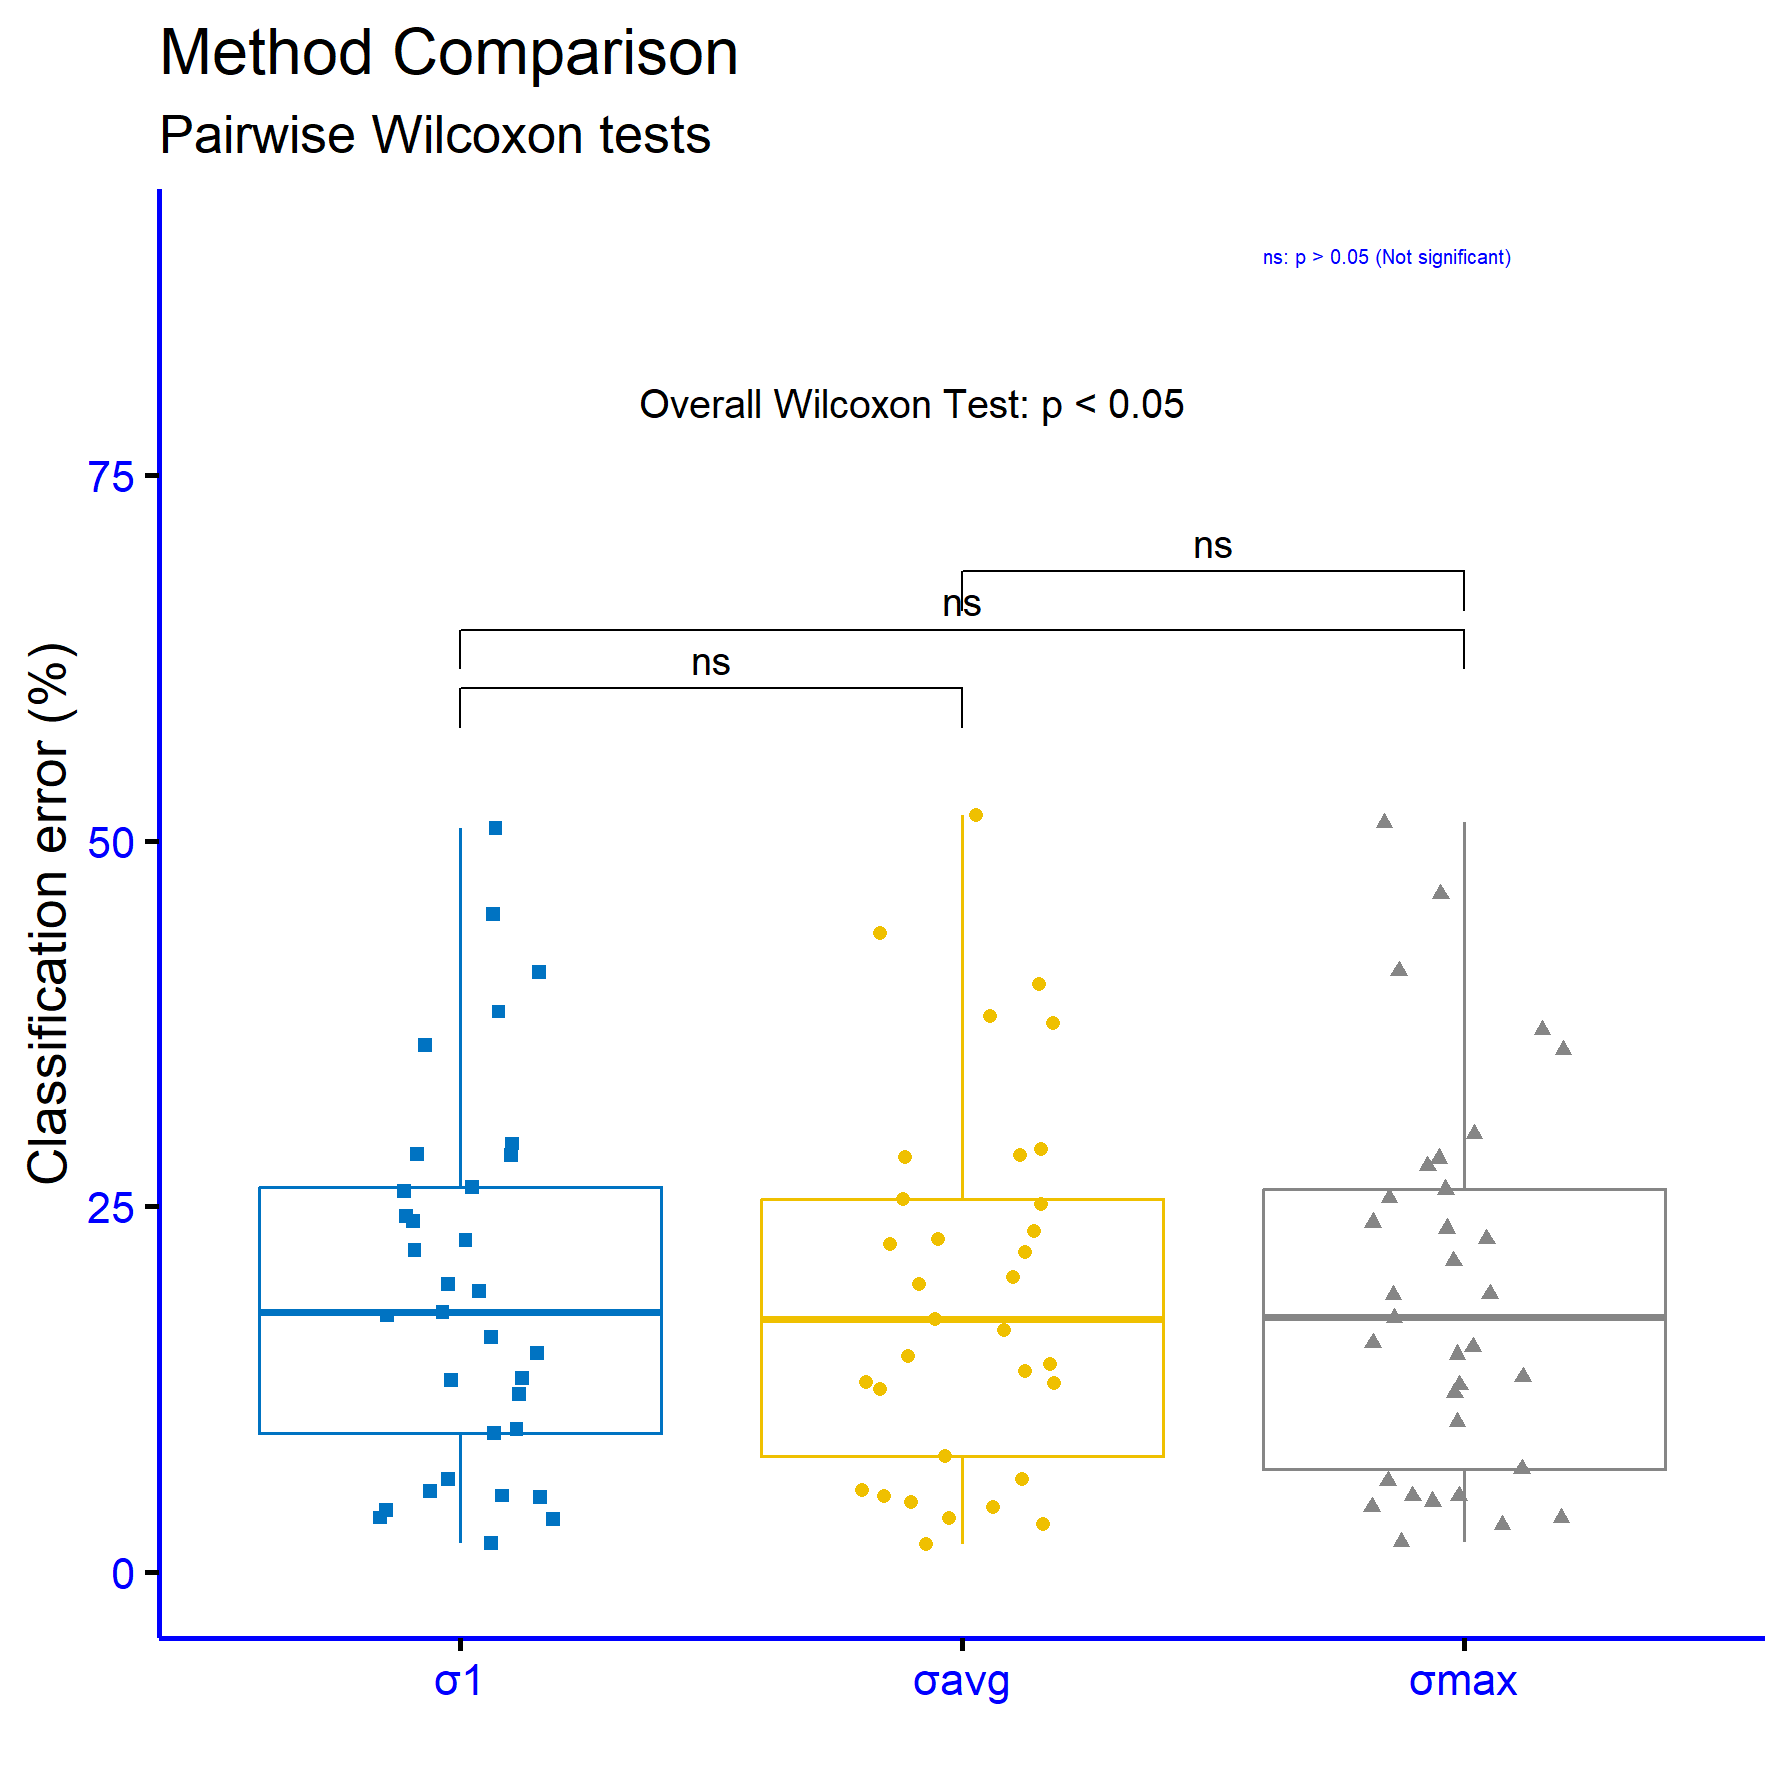
\includegraphics[scale=0.75]{stat5}

\caption{Statistical evaluation of the outcomes from applying the proposed
method to the classification datasets, considering various approaches
for determining the range of $\sigma$ parameters in the radial basis
functions.\protect\label{fig:statClassSigma}}

\end{figure}

The significance levels for comparisons of various methods for computing
the $\sigma$ parameters in the radial basis functions of the proposed
model, using the regression datasets, are presented in Figure \ref{fig:statRegressionSigma}.\textbf{
}The comparisons examined $\sigma_{1}$ vs $\sigma_{\mbox{avg}}$,
$\sigma_{1}$ vs $\sigma_{\mbox{max}}$, and $\sigma_{\mbox{avg}}$
vs $\sigma_{\mbox{max}}$ did not show any statistically significant
differences, since in all cases $p>0.05$. This means that the choice
of computation method for the $\sigma$ parameters does not have a
substantial impact on the performance of the model in regression problems.
Therefore, it can be concluded that the model demonstrates stable
and consistent behavior regardless of which initialization technique
is applied.

\begin{figure}[H]
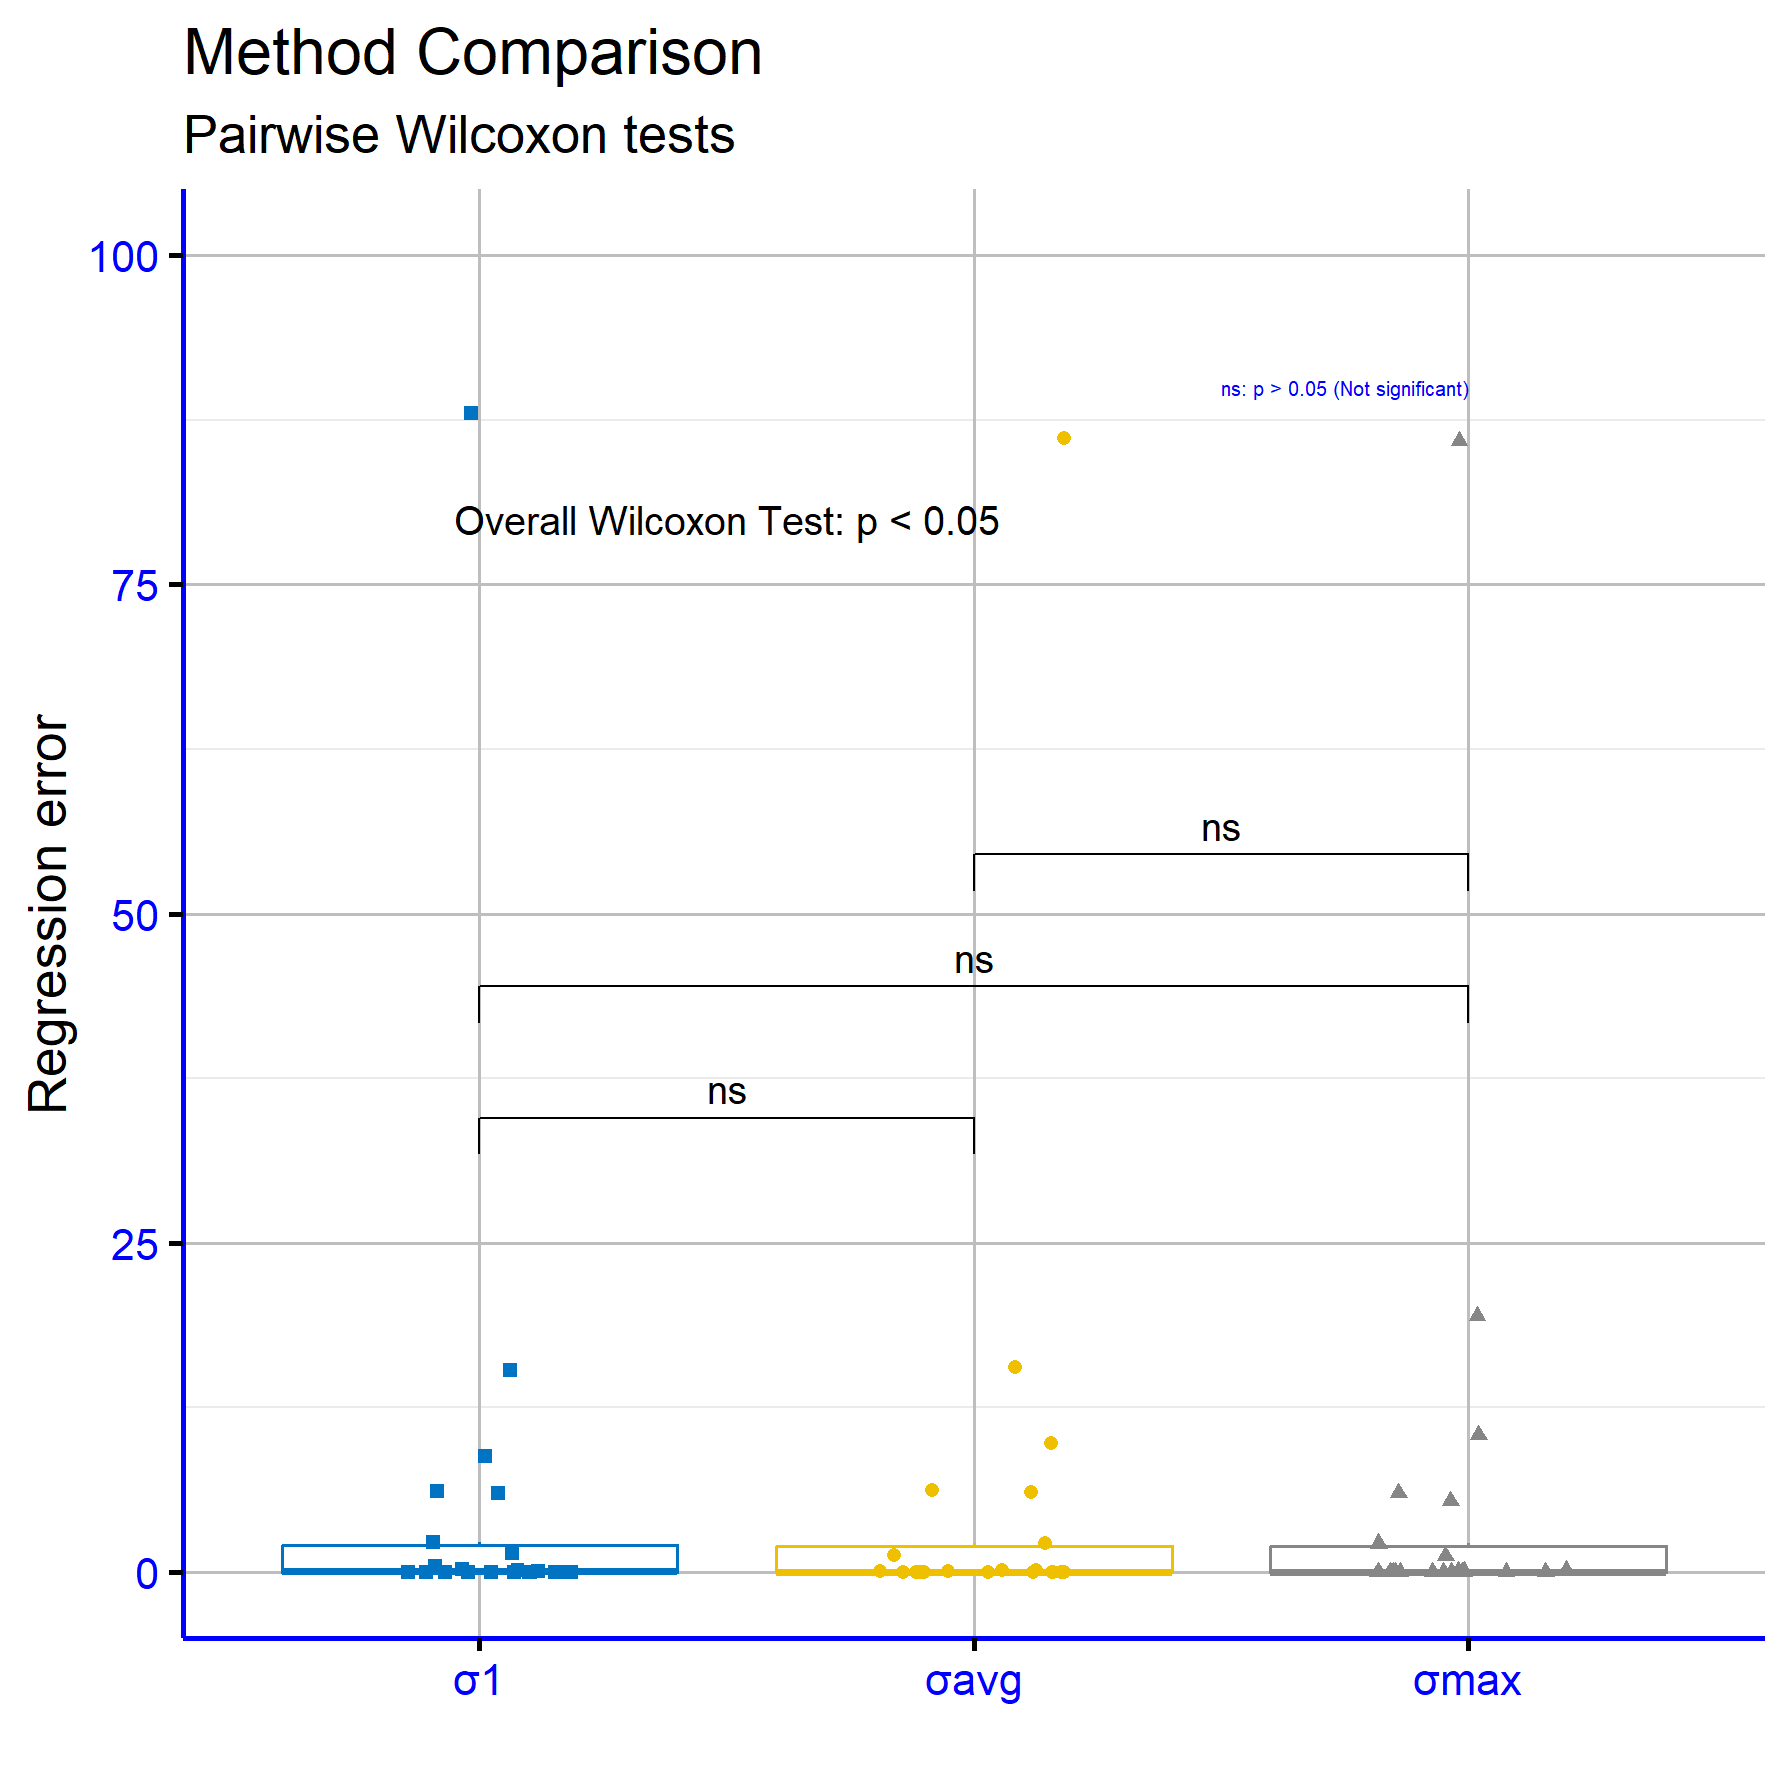
\includegraphics[scale=0.75]{stat6}

\caption{Statistical analysis of the outcomes from applying the current method
to the regression datasets, considering different approaches for determining
the range of $\sigma$ parameters in the radial functions.\protect\label{fig:statRegressionSigma}}

\end{figure}


\subsection{Experiments with the number of generations $N_{g}$ }

An additional experiment was executed, where the number of generations
was altered from $N_{g}=50$ to $N_{g}=400$ . Table \ref{tab:expClassNG}
presents the effect of the number of generations $\left(N_{g}\right)$
on the performance of the proposed model. The overall trend is downward:
the mean error decreases from 20.56\% at 50 generations to 19.46\%
at 100, essentially stabilizes at 200 with 19.45\%, and improves slightly
further at 400 to 19.11\%. Thus, the largest gain arrives early, from
50 to 100 generations (about 1.1 points), after which returns diminish,
with small but tangible additional gains. At the dataset level the
behavior varies. There are cases with clear improvements as $N_{g}$
increases, such as Alcohol (34.11\%→27.02\%), Australian (25.23\%→21.39\%),
Ionosphere (13.94\%→11.17\%), Spiral (16.66\%→12.45\%), and Z\_O\_N\_F\_S
(45.14\%→38.26\%), where more generations yield substantial benefits.
In other problems the best value occurs around 100--200 generations
and then plateaus or slightly worsens, as in Wdbc (best 4.84\% at
100), Student (4.85\% at 100), Lymography (21.64\% at 100), ZOO (8.70\%
at 100), ZONF\_S (1.98\% at 200), and Z\_F\_S (3.73\% at 200). A few
datasets show mild degradation with higher $N_{g}$, such as Wine
(7.59\%→10.24\%), Parkinsons (17.32\%→17.63\%), and to a lesser extent
Saheart, indicating that beyond a point further search is not beneficial
for all problems. Overall, 100 generations deliver the major error
reduction and represent an efficient “sweet spot,” while 200--400
generations extract modest additional gains and, in some datasets,
meaningful improvements, at the cost of more computation and occasional
local regressions.

\begin{table}[H]
\caption{The proposed method was applied to the classification datasets, and
results were analyzed for varying numbers of generations $N_{g}$
ranging from 50 to 400. \protect\label{tab:expClassNG}}

\centering{}%
\begin{tabular}{|c|c|c|c|c|}
\hline 
\textbf{DATASET} & $N_{g}=50$ & $N_{g}=100$ & \textbf{$N_{g}=200$} & $N_{g}=400$\tabularnewline
\hline 
\hline 
Alcohol & 34.11\% & 31.32\% & 28.57\% & \textbf{27.02\%}\tabularnewline
\hline 
Appendicitis & 14.90\% & \textbf{14.30\%} & 15.00\% & 14.90\%\tabularnewline
\hline 
Australian & 25.23\% & 24.96\% & 22.67\% & \textbf{21.39\%}\tabularnewline
\hline 
Balance & 14.98\% & 14.11\% & \textbf{13.11\%} & 13.52\%\tabularnewline
\hline 
Cleveland & 52.00\% & 51.31\% & \textbf{50.86\%} & 51.38\%\tabularnewline
\hline 
Circular & \textbf{3.75\%} & 3.82\% & 5.13\% & 3.82\%\tabularnewline
\hline 
Dermatology & 47.86\% & 36.29\% & \textbf{36.00\%} & 36.46\%\tabularnewline
\hline 
Hayes Roth & 40.54\% & \textbf{36.77\%} & 38.31\% & 36.77\%\tabularnewline
\hline 
Heart & 16.19\% & 16.37\% & \textbf{16.07\%} & 16.26\%\tabularnewline
\hline 
HeartAttack & 21.30\% & 21.63\% & \textbf{19.20\%} & 20.07\%\tabularnewline
\hline 
HouseVotes & 4.09\% & 3.65\% & 3.65\% & \textbf{3.61\%}\tabularnewline
\hline 
Ionosphere & 13.94\% & 12.57\% & 12.17\% & \textbf{11.17\%}\tabularnewline
\hline 
Liverdisorder & \textbf{29.06\%} & 29.23\% & 29.29\% & 29.06\%\tabularnewline
\hline 
Lymography & 22.14\% & \textbf{21.64\%} & 24.36\% & 21.86\%\tabularnewline
\hline 
Mammographic & \textbf{17.19\%} & 17.25\% & 17.79\% & 17.78\%\tabularnewline
\hline 
Parkinsons & 17.32\% & \textbf{17.11\%} & 17.53\% & 17.63\%\tabularnewline
\hline 
Pima & 24.07\% & 24.38\% & \textbf{24.02\%} & 24.28\%\tabularnewline
\hline 
Popfailures & 6.63\% & \textbf{5.92\%} & 6.33\% & 6.15\%\tabularnewline
\hline 
Regions2 & \textbf{26.02\%} & 26.14\% & 26.29\% & 26.13\%\tabularnewline
\hline 
Saheart & \textbf{28.28\%} & 28.63\% & 28.50\% & 29.61\%\tabularnewline
\hline 
Segment & 43.28\% & 42.70\% & 45.00\% & \textbf{41.35\%}\tabularnewline
\hline 
Sonar & 22.65\% & \textbf{21.20\%} & 22.00\% & 22.20\%\tabularnewline
\hline 
Spiral & 16.66\% & 14.47\% & 13.26\% & \textbf{12.45\%}\tabularnewline
\hline 
Statheart & 20.22\% & 20.67\% & 19.67\% & \textbf{19.63\%}\tabularnewline
\hline 
Student & 4.98\% & \textbf{4.85\%} & 5.23\% & 5.45\%\tabularnewline
\hline 
Transfusion & 25.47\% & \textbf{25.32\%} & 26.04\% & 25.84\%\tabularnewline
\hline 
Wdbc & 5.14\% & \textbf{4.84\%} & 5.54\% & 5.39\%\tabularnewline
\hline 
Wine & \textbf{7.59\%} & 8.53\% & 9.47\% & 10.24\%\tabularnewline
\hline 
Z\_F\_S & 4.13\% & 4.10\% & \textbf{3.73\%} & 4.40\%\tabularnewline
\hline 
Z\_O\_N\_F\_S & 45.14\% & 43.04\% & 41.00\% & \textbf{38.26\%}\tabularnewline
\hline 
ZO\_NF\_S & 4.14\% & \textbf{4.00\%} & 4.24\% & 4.02\%\tabularnewline
\hline 
ZONF\_S & 2.30\% & 2.36\% & \textbf{1.98\%} & 2.02\%\tabularnewline
\hline 
ZOO & 17.10\% & \textbf{8.70\%} & 9.80\% & 10.60\%\tabularnewline
\hline 
\textbf{AVERAGE} & \textbf{20.56\%} & \textbf{19.46\%} & \textbf{19.45\%} & \textbf{19.11\%}\tabularnewline
\hline 
\end{tabular}
\end{table}
Table \ref{tab:expRegressionNG} examines the effect of the number
of generations $\left(N_{g}\right)$ on the performance of the proposed
regression model. At the level of average error, the best value appears
at 100 generations with 5.61, marginally better than 50 generations
at 5.65, while at 200 and 400 generations the mean error increases
slightly to 5.87 and 5.86, respectively. This suggests that most of
the benefit is achieved early and that further increasing the number
of generations does not yield systematic improvement and may even
introduce a small deterioration in overall performance.

Across individual datasets the picture is heterogeneous. Clear improvements
with more generations are observed in Abalone, where the error steadily
drops to 5.88 at 400 generations, in Friedman, with a continuous decline
to 5.66, in Stock, improving to 1.33, and in Treasury, where performance
stabilizes at 0.47 from 200 generations onward. In other problems
the “sweet spot” is around 200 generations: for example, in Mortgage
the error falls from 0.66 to 0.23 at 200 before rising again, in Housing
it improves to 15.36 at 200 but worsens at 400, in BL the minimum
0.0004 occurs at 200, and in Concrete and HO there is a small but
real improvement near 200. There are also cases where more generations
seem to burden performance, such as Baseball and BK, where the error
rises as $N_{g}$ increases. In several datasets the number of generations
has little practical effect, with near-constant values in Airfoil,
Quake, SN, and PL and only minor fluctuations in Dee, FA, Laser, and
FY.

Overall, 100 generations provide an efficient and safe choice with
the lowest mean error, while 200 generations can deliver the best
results on specific datasets at the risk of small regressions elsewhere.
Further increasing to 400 generations does not offer a general gain
and may lead to slight degradation in some problems, pointing to diminishing
returns and possible overfitting or instability depending on the dataset.
\begin{table}[H]
\caption{Results obtained by applying the proposed method to the regression
datasets, while varying the number of generations $N_{g}$ \LyXZeroWidthSpace{}
between 50 and 400. \protect\label{tab:expRegressionNG}}

\centering{}%
\begin{tabular}{|c|c|c|c|c|}
\hline 
\textbf{DATASET} & $N_{g}=50$ & $N_{g}=100$ & \textbf{$N_{g}=200$} & $N_{g}=400$\tabularnewline
\hline 
Abalone & 6.35 & 6.11 & 6.12 & \textbf{5.88}\tabularnewline
\hline 
Airfoil & \textbf{0.004} & 0.004 & 0.004 & 0.004\tabularnewline
\hline 
Auto & 10.27 & 9.49 & \textbf{8.81} & 9.65\tabularnewline
\hline 
Baseball & \textbf{78.73} & 79.89 & 88.05 & 84.40\tabularnewline
\hline 
BK & \textbf{0.021} & 0.021 & 0.022 & 0.025\tabularnewline
\hline 
BL & 0.006 & 0.003 & \textbf{0.0004} & 0.006\tabularnewline
\hline 
Concrete & 0.006 & 0.006 & \textbf{0.005} & 0.005\tabularnewline
\hline 
Dee & 0.15 & 0.16 & \textbf{0.15} & 0.16\tabularnewline
\hline 
Housing & 15.96 & 15.82 & \textbf{15.36} & 18.53\tabularnewline
\hline 
Friedman & 7.41 & 6.54 & 5.99 & \textbf{5.66}\tabularnewline
\hline 
FA & \textbf{0.012} & 0.013 & 0.013 & 0.013\tabularnewline
\hline 
FY & 0.055 & 0.055 & \textbf{0.054} & 0.057\tabularnewline
\hline 
HO & 0.01 & 0.01 & \textbf{0.009} & 0.01\tabularnewline
\hline 
Laser & 0.017 & \textbf{0.015} & 0.016 & 0.015\tabularnewline
\hline 
Mortgage & 0.66 & 0.66 & \textbf{0.23} & 0.48\tabularnewline
\hline 
PL & \textbf{0.023} & 0.023 & 0.023 & 0.023\tabularnewline
\hline 
Plastic & 2.28 & 2.29 & \textbf{2.28} & 2.28\tabularnewline
\hline 
PY & 0.02 & 0.023 & 0.021 & \textbf{0.02}\tabularnewline
\hline 
Quake & \textbf{0.036} & 0.036 & 0.036 & 0.036\tabularnewline
\hline 
SN & \textbf{0.026} & 0.026 & 0.026 & 0.026\tabularnewline
\hline 
Stock & 1.70 & 1.57 & 1.44 & \textbf{1.33}\tabularnewline
\hline 
Treasury & 0.65 & 0.61 & \textbf{0.47} & 0.47\tabularnewline
\hline 
\textbf{AVERAGE} & \textbf{5.65} & \textbf{5.61} & \textbf{5.87} & \textbf{5.86}\tabularnewline
\hline 
\end{tabular}
\end{table}

Figure \ref{fig:statClassNG} shows that increasing the number of
generations from $N_{g}=50$ to $N_{g}=100$ yields a statistically
significant improvement ($p<0.01$, {*}{*}), indicating a meaningful
reduction in error in this range. By contrast, the comparisons $N_{g}=100$
vs $N_{g}=200$ and $N_{g}=200$ vs $N_{g}=400$ are not statistically
significant ($p>0.05$, ns), which means that further increasing generations
beyond 100 does not produce a consistent additional gain in performance.
Overall, the results suggest that the main benefit is achieved early
up to about 100 generations after which returns diminish and the differences
are not statistically meaningful.

\begin{figure}[H]
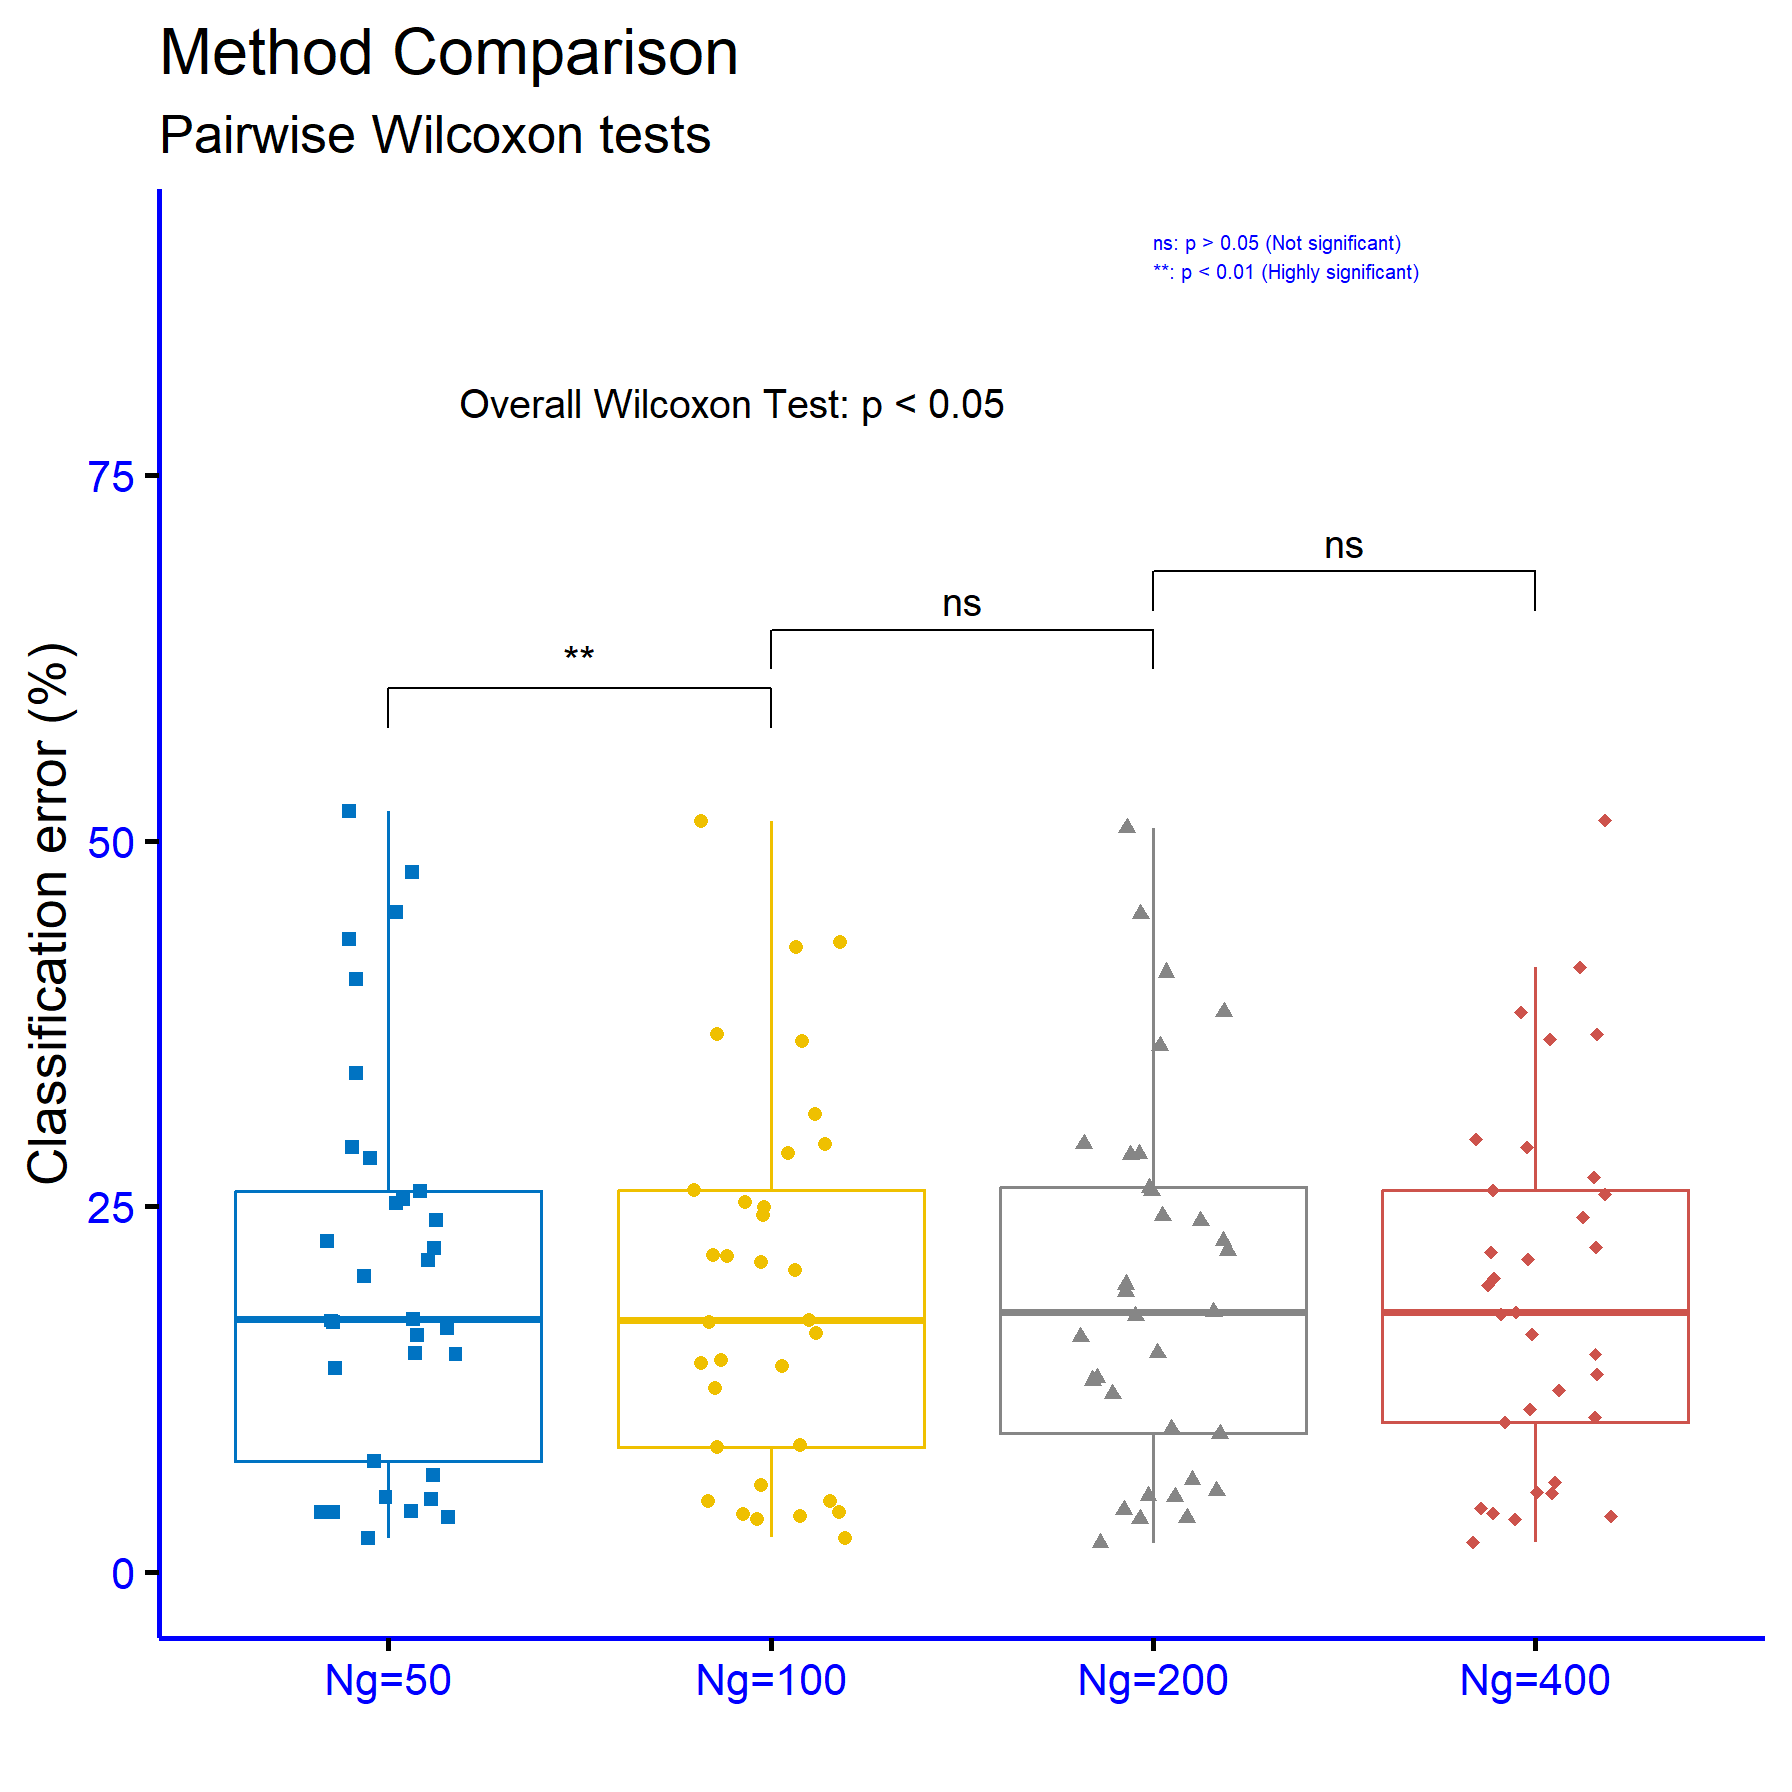
\includegraphics[scale=0.5]{stat10}

\caption{Statistical evaluation of the outcomes from applying the proposed
method to the classification datasets, with different settings of
the parameter $N_{g}$. \protect\label{fig:statClassNG}}

\end{figure}
In Figure \ref{fig:statRegressionNG}, the p-value analysis on the
regression datasets shows that the comparison between $N_{g}=50$
and $N_{g}=100$ is not statistically significant ($p>0.05$, ns),
so increasing generations in this range does not yield a consistent
improvement. By contrast, moving from $N_{g}=100$ to $N_{g}=200$
is statistically significant ($p<0.05$, {*}), indicating a measurable
reduction in error around 200 generations. Finally, the comparison
between $N_{g}=200$ and $N_{g}=400$ is not statistically significant
($p>0.05$, ns), suggesting diminishing returns beyond 200 generations.
Overall, the findings indicate that for regression problems the benefit
concentrates around 200 generations, while further increases in $N_{g}$
do not guarantee additional consistent gains.
\begin{figure}[H]
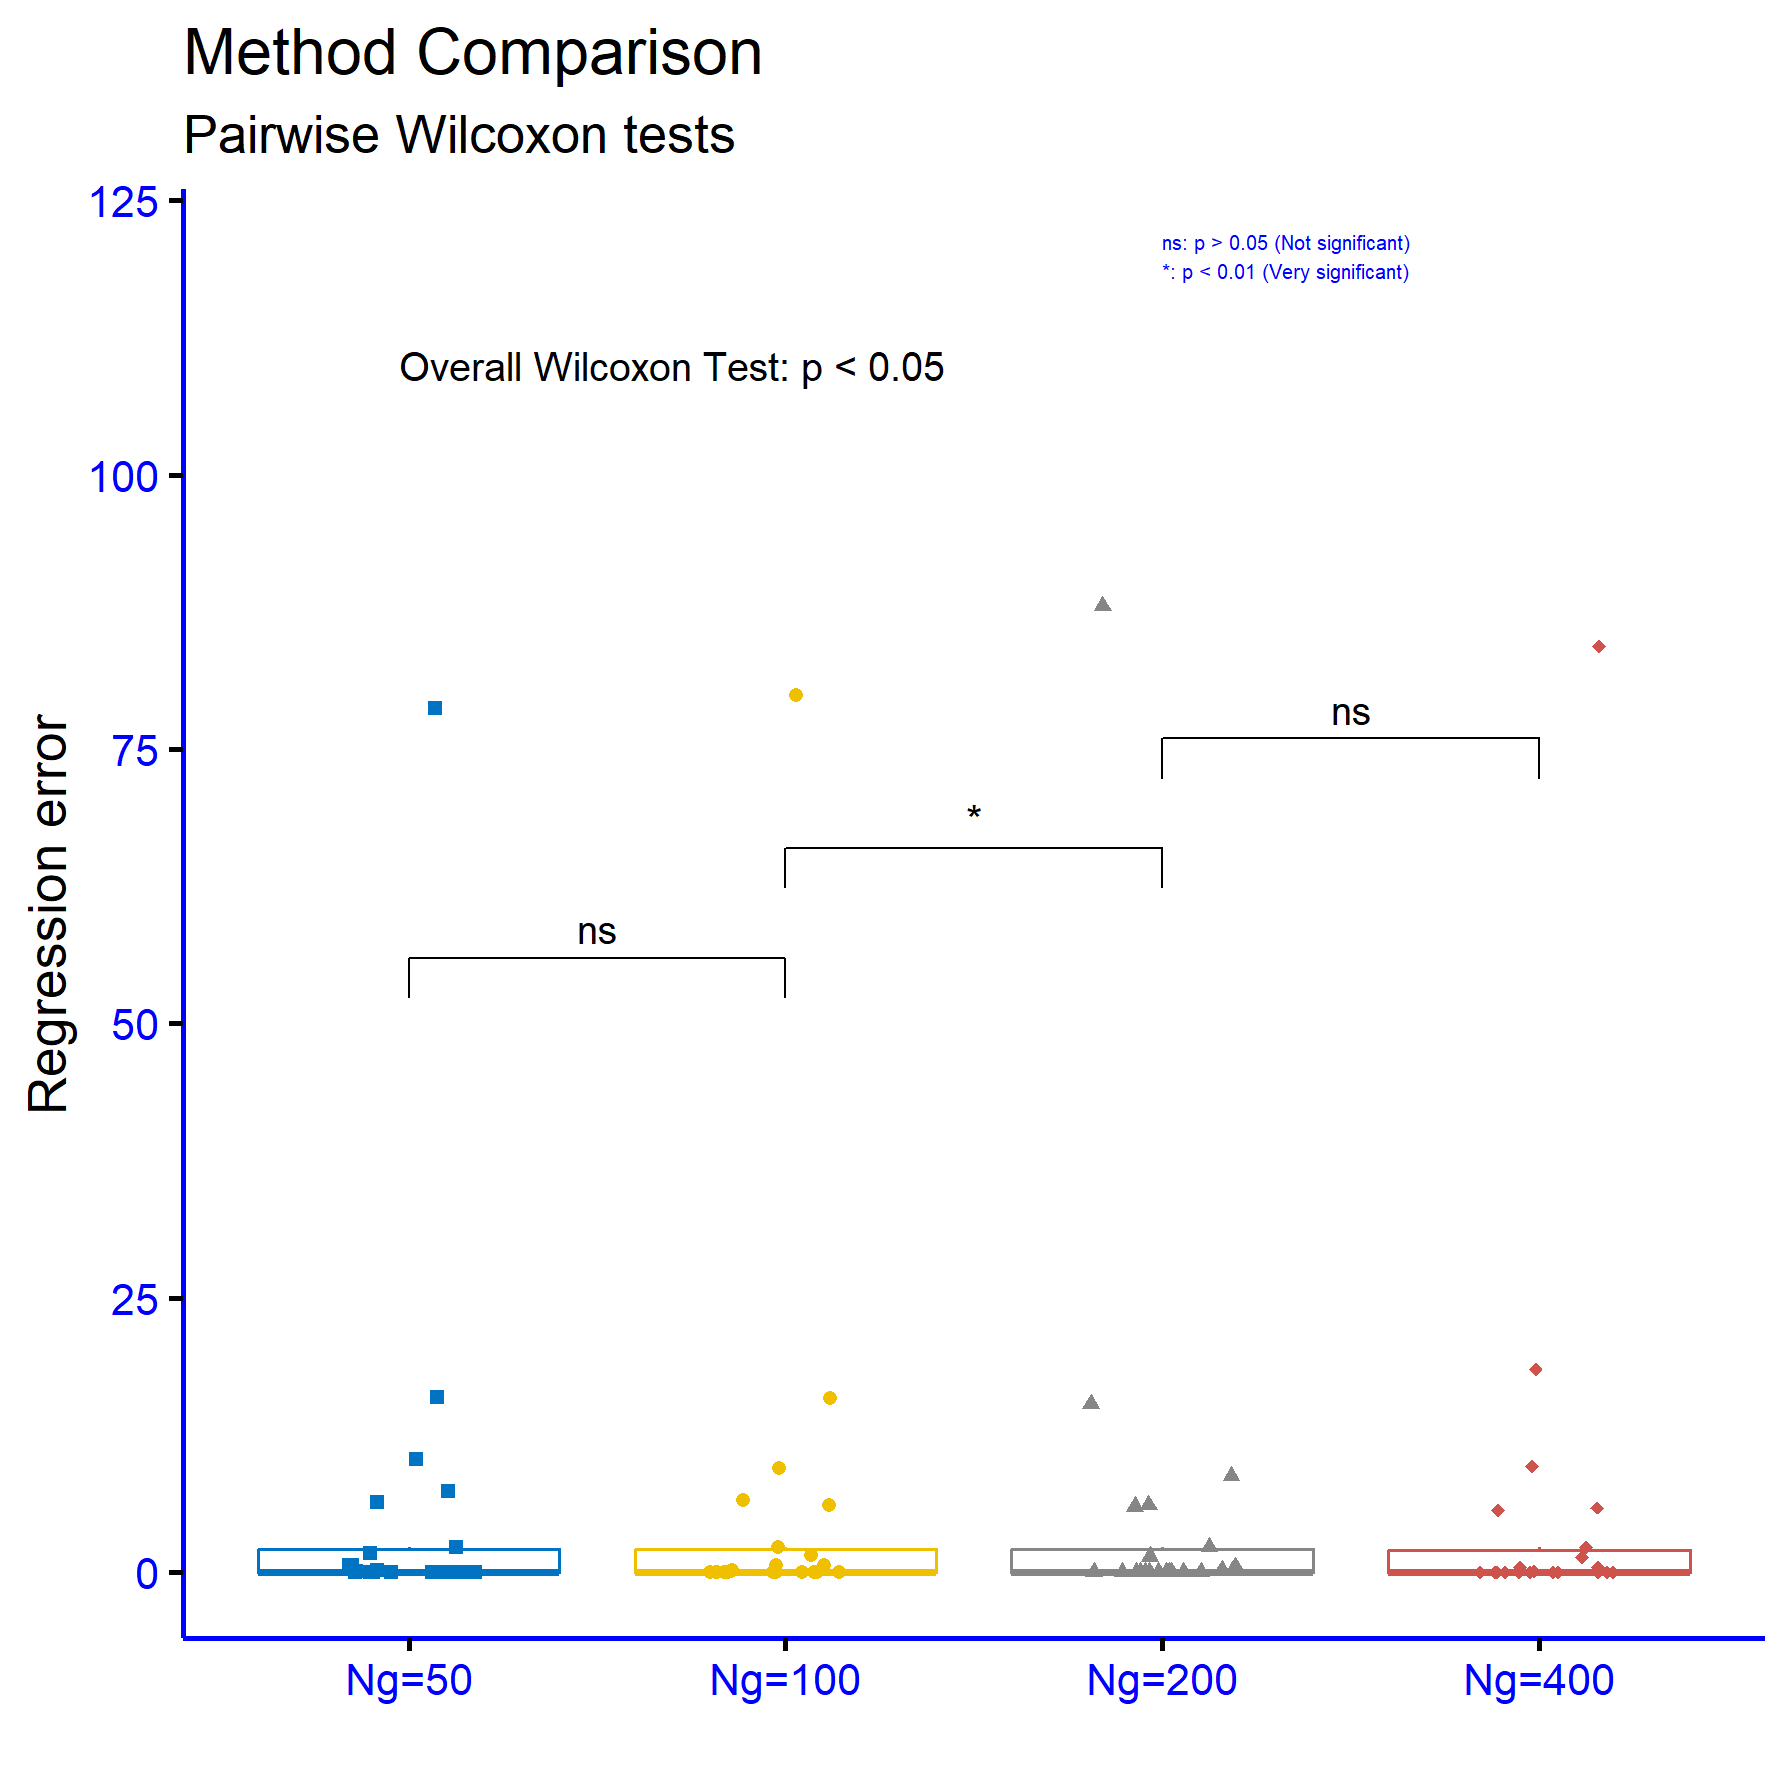
\includegraphics[scale=0.5]{stat11}

\caption{Statistical evaluation of the outcomes from applying the proposed
method to the regression datasets, with different settings of the
parameter $N_{g}$. \protect\label{fig:statRegressionNG}}

\end{figure}


\subsection{Experiments with real - world problems}

A practical problem addressed in this context is the prediction of
forest fire duration, which has been recently investigated for the
Greek region\citep{mlfire}. An experiment was conducted using data
from the Greek Fire Service to predict forest fire durations over
the period 2014--2024. In this experiment, the following methods
were used:
\begin{enumerate}
\item A neural network with 10 computing nodes, trained using the BFGS optimizer.
\item A Radial Basis Function with 10 weights, trained with the original
method for RBF training.
\item The proposed method.
\end{enumerate}
The results for the prediction of the duration are graphically illustrated
in Figure \ref{fig:experFire}. As is evident from the graph, in almost
all years the classification error of the proposed technique is lower
than the other two machine learning techniques.

\begin{figure}[H]
\begin{centering}
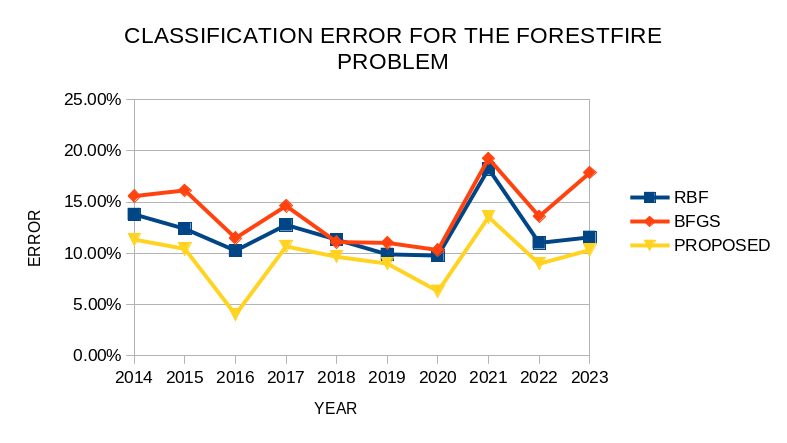
\includegraphics[scale=0.75]{rbf3_dasi}
\par\end{centering}
\caption{Average classification error for the years 2014-2023 for the forest
fires in the Greek territory. \protect\label{fig:experFire}}

\end{figure}

The second real - world example is the PIRvision dataset \citep{pirvision}
with 15302 patterns and then every pattern has 59 features. The same
machine learning models were also used in the case and the average
classification error for these methods is depicted graphically in
Figure \ref{fig:pirvision}. One more time, the proposed method has
lower classification error than the other methods involved in this
experiment.

\begin{figure}[H]
\begin{centering}
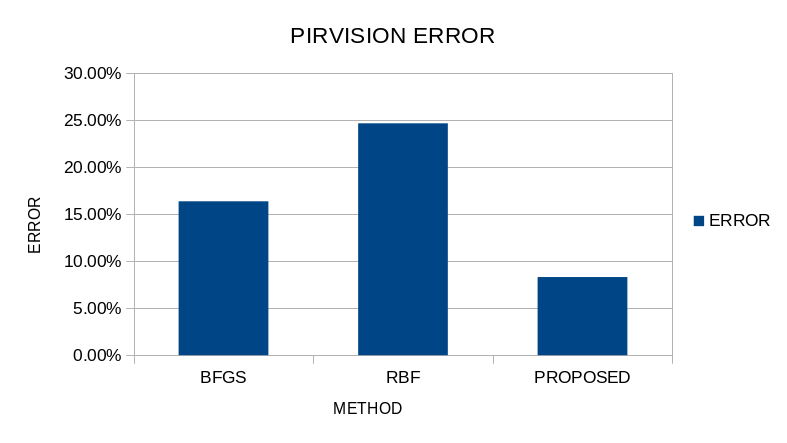
\includegraphics[scale=0.75]{rbf3_pirvision}
\par\end{centering}
\caption{The experimental results for the PIRvision dataset.\protect\label{fig:pirvision}}
\end{figure}


\section{Conclusions\protect\label{sec:Conclusions}}

The final experimental evidence shows that the three-phase RBF training
pipeline bound construction via K-means, global search with a GA inside
those bounds, and local refinement with BFGS yields robust gains across
heterogeneous classification and regression tasks. On classification,
it achieves the lowest mean error (19.45\%) with extremely significant
superiority over all baselines $\left(p<0.0001\right)$, on regression,
it attains the smallest mean absolute error (5.87), with $p<0.01$
against BFGS/ADAM and $p<0.0001$ against NEAT/RBF-KMEANS/GENRBF.
These results indicate that coupling broad exploration with constrained,
precise local tuning mitigates numerical instability and local minima,
providing reproducible performance improvements. 

Sensitivity analyses reveal that the scale factor $F$ materially
affects classification at small-to-intermediate settings ($F=1\rightarrow2$
and $F=2\rightarrow4$ are significant at $p<0.01$), with no meaningful
gain from $F=4$ to $F=8$, whereas for regression the $F$ comparisons
are not significant, highlighting methodological stability. Alternative
$\sigma$ computation methods $\left(\sigma_{1},\ \sigma_{\mbox{avg}},\ \sigma_{\mbox{max}}\right)$
differ only marginally on average and show no significant differences
in either task, reinforcing the method’s resilience to low-level design
choices. 

Automating architecture and hyperparameter adaptation is a natural
next step. Joint optimization of the number of RBF units, $F$, and
bounds via Bayesian optimization or meta-learning could reduce manual
tuning and improve generalization. Exploring alternative global optimizers
(e.g., DE, PSO, CMA-ES) or hybrid GA and Bayesian strategies may accelerate
convergence and enhance exploration, while in the final stage L-BFGS,
bound-aware variants, and stochastic formulations could benefit large-scale,
high-dimensional settings. A thorough ablation study to quantify each
phase’s contribution, along with broader post-hoc statistics, would
strengthen the evidence base. From a systems perspective, parallel/distributed
GA evaluations and GPU-accelerated RBF computations can materially
cut runtime. Finally, extending benchmarks to strong non-RBF baselines
and integrating the approach into AutoML pipelines together with analyses
of interpretability and predictive uncertainty will provide a more
complete picture of the method’s limits and potential.

It is important to note that, although highly effective, the proposed
method is more computationally intensive than other machine learning
approaches because of the sequential application of its three training
stages. Specifically, the second stage, which applies the genetic
algorithm, requires considerable computational effort. This overhead,
however, can be mitigated by leveraging modern parallel computing
techniques like OpenMP \citep{gen_openmp} or MPI \citep{gen_mpi}
.

\vspace{6pt}


\authorcontributions{V.C. and I.G.T. conducted the experiments, employing several datasets
and provided the comparative experiments. D.T. and V.C. performed
the statistical analysis and prepared the manuscript. All authors
have read and agreed to the published version of the manuscript.}

\funding{This research received no external funding.}

\institutionalreview{Not applicable.}

\informedconsent{Not applicable.}

\acknowledgments{This research has been financed by the European Union : Next Generation
EU through the Program Greece 2.0 National Recovery and Resilience
Plan , under the call RESEARCH -- CREATE -- INNOVATE, project name
“iCREW: Intelligent small craft simulator for advanced crew training
using Virtual Reality techniques\textquotedbl{} (project code:TAEDK-06195).}

\conflictsofinterest{The authors declare no conflicts of interest.}

\appendix

\begin{adjustwidth}{-\extralength}{0cm}{}

\reftitle{References}
\begin{thebibliography}{99}
\bibitem[(2006)]{physics_ml1} Raissi, M., \& Karniadakis, G. E. (2018).
Hidden physics models: Machine learning of nonlinear partial differential
equations. Journal of Computational Physics, 357, 125-141.

\bibitem{physics_ml2}Kashinath, K., Mustafa, M., Albert, A., Wu,
J. L., Jiang, C., Esmaeilzadeh, S., ... \& Prabhat, N. (2021). Physics-informed
machine learning: case studies for weather and climate modelling.
Philosophical Transactions of the Royal Society A, 379(2194), 20200093.

\bibitem[(2006)]{astronomy_ml1}Viquar, M., Basak, S., Dasgupta, A.,
Agrawal, S., \& Saha, S. (2019). Machine learning in astronomy: A
case study in quasar-star classification. Emerging Technologies in
Data Mining and Information Security: Proceedings of IEMIS 2018, Volume
3, 827-836.

\bibitem[(2006)]{astronomy_ml2}Luo, S., Leung, A. P., Hui, C. Y.,
\& Li, K. L. (2020). An investigation on the factors affecting machine
learning classifications in gamma-ray astronomy. Monthly Notices of
the Royal Astronomical Society, 492(4), 5377-5390.

\bibitem[(2006)]{chemistry_ml1}Meuwly, M. (2021). Machine learning
for chemical reactions. Chemical Reviews, 121(16), 10218-10239.

\bibitem{chemistry_ml2}J.A. Aguiar, M.L. Gong, T.Tasdizen, Crystallographic
prediction from diffraction and chemistry data for higher throughput
classification using machine learning, Computational Materials Science
\textbf{173}, 109409, 2020.

\bibitem[(2006)]{med_ml1}S.S. Yadav, S.M. Jadhav, Deep convolutional
neural network based medical image classification for disease diagnosis.
J Big Data \textbf{6}, 113, 2019.

\bibitem{med_ml2}L. Qing, W. Linhong , D. Xuehai, A Novel Neural
Network-Based Method for Medical Text Classification, Future Internet
\textbf{11}, 255, 2019. 

\bibitem[(2006)]{econ_ml1}Athey, S. (2018). The impact of machine
learning on economics. In The economics of artificial intelligence:
An agenda (pp. 507-547). University of Chicago Press.

\bibitem{econ_ml2}R. Hafezi, J. Shahrabi, E. Hadavandi, A bat-neural
network multi-agent system (BNNMAS) for stock price prediction: Case
study of DAX stock price, Applied Soft Computing \textbf{29}, pp.
196-210, 2015.

\bibitem{nn_image}Ghai, D., Tripathi, S. L., Saxena, S., Chanda,
M., \& Alazab, M. (Eds.). (2022). Machine learning algorithms for
signal and image processing. John Wiley \& Sons.

\bibitem{nn_timeseries}Ahmed, N. K., Atiya, A. F., Gayar, N. E.,
\& El-Shishiny, H. (2010). An empirical comparison of machine learning
models for time series forecasting. Econometric reviews, 29(5-6),
594-621.

\bibitem[(2006)]{rbfface}Radha, V., \& Nallammal, N. (2011, October).
Neural network based face recognition using RBFN classifier. In Proceedings
of the world congress on engineering and computer science (Vol. 1,
pp. 19-21).

\bibitem[(2006)]{rbfde1}Kumar, M., \& Yadav, N. (2011). Multilayer
perceptrons and radial basis function neural network methods for the
solution of differential equations: a survey. Computers \& Mathematics
with Applications, 62(10), 3796-3811.

\bibitem{rbfde2}Zhang, Y. (2019). An accurate and stable RBF method
for solving partial differential equations. Applied Mathematics Letters,
97, 93-98.

\bibitem[(2006)]{rbfstock}Dash, R., \& Dash, P. K. (2015, October).
A comparative study of radial basis function network with different
basis functions for stock trend prediction. In 2015 IEEE Power, Communication
and Information Technology Conference (PCITC) (pp. 430-435). IEEE.

\bibitem[(2006)]{rbfrobotics1}R. -J. Lian, Adaptive Self-Organizing
Fuzzy Sliding-Mode Radial Basis-Function Neural-Network Controller
for Robotic Systems, IEEE Transactions on Industrial Electronics \textbf{61},
pp. 1493-1503, 2014.

\bibitem{rbfrobotics2}M. Vijay, D. Jena, Backstepping terminal sliding
mode control of robot manipulator using radial basis functional neural
networks. Computers \& Electrical Engineering \textbf{67}, pp. 690-707,
2018.

\bibitem[(2006)]{rbf_dos1}U. Ravale, N. Marathe, P. Padiya, Feature
Selection Based Hybrid Anomaly Intrusion Detection System Using K
Means and RBF Kernel Function, Procedia Computer Science \textbf{45},
pp. 428-435, 2015.

\bibitem{rbf_dos2}M. Lopez-Martin, A. Sanchez-Esguevillas, J. I.
Arribas, B. Carro, Network Intrusion Detection Based on Extended RBF
Neural Network With Offline Reinforcement Learning, IEEE Access \textbf{9},
pp. 153153-153170, 2021.

\bibitem[(2006)]{rbf_process}J. A. Leonard and M. A. Kramer, \textquotedbl Radial
basis function networks for classifying process faults,\textquotedbl{}
in IEEE Control Systems Magazine, vol. 11, no. 3, pp. 31-38, April
1991, doi: 10.1109/37.75576.

\bibitem[(2006)]{rbf_time}Gan, M., Peng, H., \& Dong, X. P. (2012).
A hybrid algorithm to optimize RBF network architecture and parameters
for nonlinear time series prediction. Applied Mathematical Modelling,
36(7), 2911-2919.

\bibitem[(2006)]{rbf_wind}G. Sideratos and N. Hatziargyriou, \textquotedbl Using
Radial Basis Neural Networks to Estimate Wind Power Production,\textquotedbl{}
2007 IEEE Power Engineering Society General Meeting, Tampa, FL, USA,
2007, pp. 1-7, doi: 10.1109/PES.2007.385812.

\bibitem[(2006)]{kmeans}MacQueen, J.: Some methods for classification
and analysis of multivariate observations, in: Proceedings of the
fifth Berkeley symposium on mathematical statistics and probability,
Vol. 1, No. 14, pp. 281-297, 1967. 

\bibitem[(2006)]{rbf_universal}J. Park and I. W. Sandberg, \textquotedbl Universal
Approximation Using Radial-Basis-Function Networks,\textquotedbl{}
in Neural Computation, vol. 3, no. 2, pp. 246-257, June 1991, doi:
10.1162/neco.1991.3.2.246. 

\bibitem[(2006)]{rbfinit1}L.I. Kuncheva, Initializing of an RBF network
by a genetic algorithm, Neurocomputing \textbf{14}, pp. 273-288, 1997.

\bibitem{rbfinit2}F. Ros, M. Pintore, A. Deman, J.R. Chrétien, Automatical
initialization of RBF neural networks, Chemometrics and Intelligent
Laboratory Systems \textbf{87}, pp. 26-32, 2007.

\bibitem{rbfinit3}D. Wang, X.J. Zeng, J.A. Keane, A clustering algorithm
for radial basis function neural network initialization, Neurocomputing
\textbf{77}, pp. 144-155, 2012.

\bibitem[(2006)]{rbfkernel}N. Benoudjit, M. Verleysen, On the Kernel
Widths in Radial-Basis Function Networks, Neural Processing Letters
\textbf{18}, pp. 139--154, 2003.

\bibitem[(2006)]{rbfprun1}Määttä, J., Bazaliy, V., Kimari, J., Djurabekova,
F., Nordlund, K., \& Roos, T. (2021). Gradient-based training and
pruning of radial basis function networks with an application in materials
physics. Neural Networks, 133, 123-131.

\bibitem{rbfprun3}Gale, S., Vestheim, S., Gravdahl, J. T., Fjerdingen,
S., \& Schjølberg, I. (2013, July). RBF network pruning techniques
for adaptive learning controllers. In 9th International Workshop on
Robot Motion and Control (pp. 246-251). IEEE.

\bibitem{rbfprun2}M. Bortman and M. Aladjem, A Growing and Pruning
Method for Radial Basis Function Networks, IEEE Transactions on Neural
Networks \textbf{20}, pp. 1039-1045, 2009.

\bibitem[(2025)]{rbfcon1}Du, J. X., Huang, D. S., Zhang, G. J., \&
Wang, Z. F. (2006). A novel full structure optimization algorithm
for radial basis probabilistic neural networks. Neurocomputing, 70(1-3),
592-596.

\bibitem[(2025)]{rbfcon2}Yu, H., Reiner, P. D., Xie, T., Bartczak,
T., \& Wilamowski, B. M. (2014). An incremental design of radial basis
function networks. IEEE transactions on neural networks and learning
systems, 25(10), 1793-1803.

\bibitem[(2006)]{rbfga1}Ding, S., Xu, L., Su, C., \& Jin, F. (2012).
An optimizing method of RBF neural network based on genetic algorithm.
Neural Computing and Applications, 21(2), 333-336.

\bibitem[(2006)]{rbfga2}Jia, W., Zhao, D., \& Ding, L. (2016). An
optimized RBF neural network algorithm based on partial least squares
and genetic algorithm for classification of small sample. Applied
Soft Computing, 48, 373-384.

\bibitem[(2006)]{rbfpso1}Rani R, H. J., \& Victoire T, A. A. (2018).
Training radial basis function networks for wind speed prediction
using PSO enhanced differential search optimizer. PloS one, 13(5),
e0196871.

\bibitem[(2006)]{rbfpso2}Zhang, W., \& Wei, D. (2018). Prediction
for network traffic of radial basis function neural network model
based on improved particle swarm optimization algorithm. Neural Computing
and Applications, 29(4), 1143-1152.

\bibitem[(2006)]{rbfdiff1}Qasem, S. N., Shamsuddin, S. M., \& Zain,
A. M. (2012). Multi-objective hybrid evolutionary algorithms for radial
basis function neural network design. Knowledge-Based Systems, 27,
475-497.

\bibitem{rbfpar1}R. Yokota, L.A. Barba, M. G. Knepley, PetRBF ---
A parallel O(N) algorithm for radial basis function interpolation
with Gaussians, Computer Methods in Applied Mechanics and Engineering
\textbf{199}, pp. 1793-1804, 2010.

\bibitem{rbfpar2}C. Lu, N. Ma, Z. Wang, Fault detection for hydraulic
pump based on chaotic parallel RBF network, EURASIP J. Adv. Signal
Process. \textbf{2011}, 49, 2011.

\bibitem[(2018)]{rbf_pso_new}Rani R, H. J., \& Victoire T, A. A.
(2018). Training radial basis function networks for wind speed prediction
using PSO enhanced differential search optimizer. PloS one, 13(5),
e0196871.

\bibitem[(2018)]{rbf_variable_projection}Karamichailidou, D., Gerolymatos,
G., Patrinos, P., Sarimveis, H., \& Alexandridis, A. (2024). Radial
basis function neural network training using variable projection and
fuzzy means. Neural Computing and Applications, 36(33), 21137-21151.

\bibitem{gen_kmeans}K. Krishna, M. Narasimha Murty, Genetic K-means
algorithm, IEEE Transactions on Systems, Man, and Cybernetics, Part
B (Cybernetics) \textbf{ 29}, pp. 433-439, 1999.

\bibitem{unsuper_kmeans}K. P. Sinaga, M. -S. Yang, Unsupervised K-Means
Clustering Algorithm, IEEE Access \textbf{8}, pp. 80716-80727, 2020. 

\bibitem{fixed_kmeans}M. Ay, L. Özbakır, S. Kulluk, B. Gülmez , G.Öztürk,
S. Özer, FC-Kmeans: Fixed-centered K-means algorithm, Expert Systems
with Applications \textbf{211}, 118656, 2023.

\bibitem{kmeans_review}E.U. Oti, M.O. Olusola, F.C. Eze, S.U. Enogwe,
Comprehensive review of K-Means clustering algorithms, Criterion \textbf{12},
pp. 22-23, 2021.

\bibitem{gen_app1}S.A. Grady, M.Y. Hussaini, M.M. Abdullah, Placement
of wind turbines using genetic algorithms, Renewable Energy \textbf{30},
pp. 259-270, 2005.

\bibitem{gen_app2}Parvaze, S., Kumar, R., Khan, J. N., Al-Ansari,
N., Parvaze, S., Vishwakarma, D. K., ... \& Kuriqi, A. (2023). Optimization
of water distribution systems using genetic algorithms: A review.
Archives of Computational Methods in Engineering, 30(7), 4209-4244.

\bibitem{gen_app3}Gordini, N. (2014). A genetic algorithm approach
for SMEs bankruptcy prediction: Empirical evidence from Italy. Expert
systems with applications, 41(14), 6433-6445.

\bibitem{gen_app4}Ding, S., Su, C., \& Yu, J. (2011). An optimizing
BP neural network algorithm based on genetic algorithm. Artificial
intelligence review, 36(2), 153-162.

\bibitem[(2004)]{pga1}Guo, L., Funie, A. I., Thomas, D. B., Fu, H.,
\& Luk, W. (2016). Parallel genetic algorithms on multiple FPGAs.
ACM SIGARCH Computer Architecture News, 43(4), 86-93.

\bibitem[(2004)]{pga2}Johar, F. M., Azmin, F. A., Suaidi, M. K.,
Shibghatullah, A. S., Ahmad, B. H., Salleh, S. N., ... \& Shukor,
M. M. (2013, November). A review of genetic algorithms and parallel
genetic algorithms on graphics processing unit (GPU). In 2013 IEEE
International Conference on Control System, Computing and Engineering
(pp. 264-269). IEEE.

\bibitem{kaelo}P. Kaelo, M.M. Ali, Integrated crossover rules in
real coded genetic algorithms, European Journal of Operational Research
\textbf{176}, pp. 60-76, 2007.

\bibitem[(2004)]{powell}M.J.D Powell, A Tolerant Algorithm for Linearly
Constrained Optimization Calculations, Mathematical Programming \textbf{45},
pp. 547-566, 1989. 

\bibitem[(2004)]{lbfgs}Liu, D. C., \& Nocedal, J. (1989). On the
limited memory BFGS method for large scale optimization. Mathematical
programming, 45(1), 503-528.

\bibitem[(2004)]{resbfgs}A. Mokhtari and A. Ribeiro, \textquotedbl RES:
Regularized Stochastic BFGS Algorithm,\textquotedbl{} in IEEE Transactions
on Signal Processing, vol. 62, no. 23, pp. 6089-6104, Dec.1, 2014,
doi: 10.1109/TSP.2014.2357775. 

\bibitem[(2004)]{conbfgs}Dai, Y. H. (2002). Convergence properties
of the BFGS algoritm. SIAM Journal on Optimization, 13(3), 693-701.

\bibitem[(1989)]{uci} M. Kelly, R. Longjohn, K. Nottingham, The UCI
Machine Learning Repository, \url{https://archive.ics.uci.edu} (accessed
on 28 September 2025).

\bibitem{Keel}J. Alcalá-Fdez, A. Fernandez, J. Luengo, J. Derrac,
S. García, L. Sánchez, F. Herrera. KEEL Data-Mining Software Tool:
Data Set Repository, Integration of Algorithms and Experimental Analysis
Framework. Journal of Multiple-Valued Logic and Soft Computing 17,
pp. 255-287, 2011. \url{https://sci2s.ugr.es/keel/datasets.php} (accessed
on 28 September 2025).

\bibitem[(2025)]{statlib}Kooperberg, C. (1997). Statlib: an archive
for statistical software, datasets, and information. The American
Statistician, 51(1), 98. \url{https://lib.stat.cmu.edu/datasets/}
(accessed on 28 September 2025).

\bibitem{appendicitis}Weiss, Sholom M. and Kulikowski, Casimir A.,
Computer Systems That Learn: Classification and Prediction Methods
from Statistics, Neural Nets, Machine Learning, and Expert Systems,
Morgan Kaufmann Publishers Inc, 1991.

\bibitem[Tzimourta(2018)]{alcohol}Tzimourta, K.D.; Tsoulos, I.; Bilero,
I.T.; Tzallas, A.T.; Tsipouras, M.G.; Giannakeas, N. Direct Assessment
of Alcohol Consumption in Mental State Using Brain Computer Interfaces
and Grammatical Evolution. Inventions 2018, 3, 51.

\bibitem[Quinlan(2018)]{australian}J.R. Quinlan, Simplifying Decision
Trees. International Journal of Man-Machine Studies \textbf{27}, pp.
221-234, 1987. 

\bibitem{balance}T. Shultz, D. Mareschal, W. Schmidt, Modeling Cognitive
Development on Balance Scale Phenomena, Machine Learning \textbf{16},
pp. 59-88, 1994.

\bibitem[(2004)]{cleveland1}Z.H. Zhou,Y. Jiang, NeC4.5: neural ensemble
based C4.5,\textquotedbl{} in IEEE Transactions on Knowledge and Data
Engineering \textbf{16}, pp. 770-773, 2004.

\bibitem{cleveland2}R. Setiono , W.K. Leow, FERNN: An Algorithm for
Fast Extraction of Rules from Neural Networks, Applied Intelligence
\textbf{12}, pp. 15-25, 2000.

\bibitem[(2008)]{fcgen}Gavrilis, D., Tsoulos, I. G., \& Dermatas,
E. (2008). Selecting and constructing features using grammatical evolution.
Pattern Recognition Letters, 29(9), 1358-1365.

\bibitem[(1998)]{dermatology}G. Demiroz, H.A. Govenir, N. Ilter,
Learning Differential Diagnosis of Eryhemato-Squamous Diseases using
Voting Feature Intervals, Artificial Intelligence in Medicine. \textbf{13},
pp. 147--165, 1998.

\bibitem[(1996)]{ecoli}P. Horton, K.Nakai, A Probabilistic Classification
System for Predicting the Cellular Localization Sites of Proteins,
In: Proceedings of International Conference on Intelligent Systems
for Molecular Biology \textbf{4}, pp. 109-15, 1996.

\bibitem[(1977)]{hayes-roth}B. Hayes-Roth, B., F. Hayes-Roth. Concept
learning and the recognition and classification of exemplars. Journal
of Verbal Learning and Verbal Behavior \textbf{16}, pp. 321-338, 1977.

\bibitem[(1997)]{heart}I. Kononenko, E. Šimec, M. Robnik-Šikonja,
Overcoming the Myopia of Inductive Learning Algorithms with RELIEFF,
Applied Intelligence \textbf{7}, pp. 39--55, 1997

\bibitem[(2022)]{heartAttack}Rashid, Tarik A.; Hassan, Bryar (2022),
“Heart Attack Dataset”, Mendeley Data, V1, doi: 10.17632/wmhctcrt5v.1

\bibitem[(2002)]{housevotes}R.M. French, N. Chater, Using noise to
compute error surfaces in connectionist networks: a novel means of
reducing catastrophic forgetting, Neural Comput. \textbf{14}, pp.
1755-1769, 2002.

\bibitem[(2004)]{ion1}J.G. Dy , C.E. Brodley, Feature Selection for
Unsupervised Learning, The Journal of Machine Learning Research \textbf{5},
pp 845--889, 2004.

\bibitem{ion2}S. J. Perantonis, V. Virvilis, Input Feature Extraction
for Multilayered Perceptrons Using Supervised Principal Component
Analysis, Neural Processing Letters \textbf{10}, pp 243--252, 1999.

\bibitem[(2002)]{liver} J. Garcke, M. Griebel, Classification with
sparse grids using simplicial basis functions, Intell. Data Anal.
\textbf{6}, pp. 483-502, 2002.

\bibitem{liver1}J. Mcdermott, R.S. Forsyth, Diagnosing a disorder
in a classification benchmark, Pattern Recognition Letters \textbf{73},
pp. 41-43, 2016.

\bibitem[(2002)]{lymography}G. Cestnik, I. Konenenko, I. Bratko,
Assistant-86: A Knowledge-Elicitation Tool for Sophisticated Users.
In: Bratko, I. and Lavrac, N., Eds., Progress in Machine Learning,
Sigma Press, Wilmslow, pp. 31-45, 1987. 

\bibitem[(2007)]{mammographic}M. Elter, R. Schulz-Wendtland, T. Wittenberg,
The prediction of breast cancer biopsy outcomes using two CAD approaches
that both emphasize an intelligible decision process, Med Phys. \textbf{34},
pp. 4164-72, 2007.

\bibitem[(2007)]{parkinsons1}M.A. Little, P.E. McSharry, S.J Roberts
et al, Exploiting Nonlinear Recurrence and Fractal Scaling Properties
for Voice Disorder Detection. BioMed Eng OnLine \textbf{6}, 23, 2007.

\bibitem{parkinsons2}M.A. Little, P.E. McSharry, E.J. Hunter, J.
Spielman, L.O. Ramig, Suitability of dysphonia measurements for telemonitoring
of Parkinson's disease. IEEE Trans Biomed Eng. \textbf{56}, pp. 1015-1022,
2009.

\bibitem[(2007)]{pima}J.W. Smith, J.E. Everhart, W.C. Dickson, W.C.
Knowler, R.S. Johannes, Using the ADAP learning algorithm to forecast
the onset of diabetes mellitus, In: Proceedings of the Symposium on
Computer Applications and Medical Care IEEE Computer Society Press,
pp.261-265, 1988.

\bibitem[(2007)]{popfailures}D.D. Lucas, R. Klein, J. Tannahill,
D. Ivanova, S. Brandon, D. Domyancic, Y. Zhang, Failure analysis of
parameter-induced simulation crashes in climate models, Geoscientific
Model Development \textbf{6}, pp. 1157-1171, 2013.

\bibitem[(2007)]{regions2}N. Giannakeas, M.G. Tsipouras, A.T. Tzallas,
K. Kyriakidi, Z.E. Tsianou, P. Manousou, A. Hall, E.C. Karvounis,
V. Tsianos, E. Tsianos, A clustering based method for collagen proportional
area extraction in liver biopsy images (2015) Proceedings of the Annual
International Conference of the IEEE Engineering in Medicine and Biology
Society, EMBS, 2015-November, art. no. 7319047, pp. 3097-3100. 

\bibitem[(2007)]{saheart}T. Hastie, R. Tibshirani, Non-parametric
logistic and proportional odds regression, JRSS-C (Applied Statistics)
\textbf{36}, pp. 260--276, 1987.

\bibitem{segment}M. Dash, H. Liu, P. Scheuermann, K. L. Tan, Fast
hierarchical clustering and its validation, Data \& Knowledge Engineering
\textbf{44}, pp 109--138, 2003.

\bibitem[(2008)]{statheart}Dua, D. and Graff, C. (2019). UCI Machine
Learning Repository {[}http://archive.ics.uci.edu/ml{]}. Irvine, CA:
University of California, School of Information and Computer Science.

\bibitem[(2007)]{student}P. Cortez, A. M. Gonçalves Silva, Using
data mining to predict secondary school student performance, In Proceedings
of 5th FUture BUsiness TEChnology Conference (FUBUTEC 2008) (pp. 5--12).
EUROSIS-ETI, 2008.

\bibitem[(2007)]{transfusion}I-Cheng Yeh, King-Jang Yang, Tao-Ming
Ting, Knowledge discovery on RFM model using Bernoulli sequence, Expert
Systems with Applications \textbf{36}, pp. 5866-5871, 2009.

\bibitem[(2007)]{wdbc1}Jeyasingh, S., \& Veluchamy, M. (2017). Modified
bat algorithm for feature selection with the Wisconsin diagnosis breast
cancer (WDBC) dataset. Asian Pacific journal of cancer prevention:
APJCP, 18(5), 1257.

\bibitem[(2007)]{wdbc2}Alshayeji, M. H., Ellethy, H., \& Gupta, R.
(2022). Computer-aided detection of breast cancer on the Wisconsin
dataset: An artificial neural networks approach. Biomedical signal
processing and control, 71, 103141.

\bibitem[(2007)]{wine1}M. Raymer, T.E. Doom, L.A. Kuhn, W.F. Punch,
Knowledge discovery in medical and biological datasets using a hybrid
Bayes classifier/evolutionary algorithm. IEEE transactions on systems,
man, and cybernetics. Part B, Cybernetics : a publication of the IEEE
Systems, Man, and Cybernetics Society, \textbf{33} , pp. 802-813,
2003.

\bibitem{wine2}P. Zhong, M. Fukushima, Regularized nonsmooth Newton
method for multi-class support vector machines, Optimization Methods
and Software \textbf{22}, pp. 225-236, 2007.

\bibitem[(2007)]{eeg1}R. G. Andrzejak, K. Lehnertz, F.Mormann, C.
Rieke, P. David, and C. E. Elger, “Indications of nonlinear deterministic
and finite-dimensional structures in time series of brain electrical
activity: dependence on recording region and brain state,” Physical
Review E, vol. 64, no. 6, Article ID 061907, 8 pages, 2001. 

\bibitem{eeg2}A. T. Tzallas, M. G. Tsipouras, and D. I. Fotiadis,
“Automatic Seizure Detection Based on Time-Frequency Analysis and
Artificial Neural Networks,” Computational Intelligence and Neuroscience,
vol. 2007, Article ID 80510, 13 pages, 2007. doi:10.1155/2007/80510

\bibitem[(2007)]{zoo}M. Koivisto, K. Sood, Exact Bayesian Structure
Discovery in Bayesian Networks, The Journal of Machine Learning Research\textbf{
5}, pp. 549--573, 2004.

\bibitem[(2007)]{abalone}Nash, W.J.; Sellers, T.L.; Talbot, S.R.;
Cawthor, A.J.; Ford, W.B. The Population Biology of Abalone (\_Haliotis\_
species) in Tasmania. I. Blacklip Abalone (\_H. rubra\_) from the
North Coast and Islands of Bass Strait, Sea Fisheries Division; Technical
Report No. 48; Department of Primary Industry and Fisheries, Tasmania:
Hobart, Australia, 1994; ISSN 1034-3288

\bibitem[(2007)]{airfoil}Brooks, T.F.; Pope, D.S.; Marcolini, A.M.
Airfoil Self-Noise and Prediction. Technical Report, NASA RP-1218.
July 1989. Available online: https://ntrs.nasa.gov/citations/19890016302
(accessed on 14 November 2024).

\bibitem[(2022)]{auto_dataset}Quinlan,R. (1993). Combining Instance-Based
and Model-Based Learning. In Proceedings on the Tenth International
Conference of Machine Learning, 236-243, University of Massachusetts,
Amherst. Morgan Kaufmann.

\bibitem[(2007)]{concrete}I.Cheng Yeh, Modeling of strength of high
performance concrete using artificial neural networks, Cement and
Concrete Research. \textbf{28}, pp. 1797-1808, 1998. 

\bibitem{friedman}Friedman, J. (1991): Multivariate Adaptative Regression
Splines. Annals of Statistics, 19:1, 1-{}-141. 

\bibitem[(2007)]{housing}D. Harrison and D.L. Rubinfeld, Hedonic
prices and the demand for clean ai, J. Environ. Economics \& Management
\textbf{5}, pp. 81-102, 1978.

\bibitem[(2025)]{optimus}I.G. Tsoulos, V. Charilogis, G. Kyrou, V.N.
Stavrou, A. Tzallas, Journal of Open Source Software \textbf{10},
7584, 2025.

\bibitem[(2025)]{bfgs}Yuan, Y. X. (1991). A modified BFGS algorithm
for unconstrained optimization. IMA Journal of Numerical Analysis,
11(3), 325-332.

\bibitem{nn1}C. Bishop, Neural Networks for Pattern Recognition,
Oxford University Press, 1995.

\bibitem{nn2}G. Cybenko, Approximation by superpositions of a sigmoidal
function, Mathematics of Control Signals and Systems \textbf{2}, pp.
303-314, 1989.

\bibitem{Adam}D. P. Kingma, J. L. Ba, ADAM: a method for stochastic
optimization, in: Proceedings of the 3rd International Conference
on Learning Representations (ICLR 2015), pp. 1--15, 2015.

\bibitem{AdamNN}Y. Xue, Y. Tong, F. Neri, An ensemble of differential
evolution and Adam for training feed-forward neural networks. Information
Sciences \textbf{608}, pp. 453-471, 2022.

\bibitem[(2025)]{neat}K. O. Stanley, R. Miikkulainen, Evolving Neural
Networks through Augmenting Topologies, Evolutionary Computation \textbf{10},
pp. 99-127, 2002.

\bibitem[(2020)]{adagrad}Ward, R., Wu, X., \& Bottou, L. (2020).
Adagrad stepsizes: Sharp convergence over nonconvex landscapes. Journal
of Machine Learning Research, 21(219), 1-30.

\bibitem[(2014)]{bayesopt}Ruben Martinez-Cantin, BayesOpt: A Bayesian
Optimization Library for Nonlinear Optimization, Experimental Design
and Bandits. Journal of Machine Learning Research, 15(Nov):3735-{}-3739,
2014.

\bibitem{rbf_gen1}S. Ding, L. Xu, C. Su et al, An optimizing method
of RBF neural network based on genetic algorithm. Neural Comput \&
Applic 21, pp. 333--336, 2012.

\bibitem[(2024)]{mlfire}C. Kopitsa, I.G. Tsoulos, V. Charilogis,
A. Stavrakoudis, Predicting the Duration of Forest Fires Using Machine
Learning Methods, Future Internet \textbf{16}, 396, 2024.

\bibitem[(2023)]{pirvision}Emad-Ud-Din, M., \& Wang, Y. (2023). Promoting
occupancy detection accuracy using on-device lifelong learning. IEEE
Sensors Journal, 23(9), 9595-9606.

\bibitem[(2019)]{gen_openmp}Saxena, R., Jain, M., Malhotra, K., \&
Vasa, K. D. (2019). An optimized openmp-based genetic algorithm solution
to vehicle routing problem. In Smart Computing Paradigms: New Progresses
and Challenges: Proceedings of ICACNI 2018, Volume 2 (pp. 237-245).
Singapore: Springer Singapore.

\bibitem[(2019)]{gen_mpi}Rajan, S. D., \& Nguyen, D. T. (2004). Design
optimization of discrete structural systems using MPI-enabled genetic
algorithm. Structural and Multidisciplinary Optimization, 28(5), 340-348.

\end{thebibliography}
%%%%%%%%%%%%%%%%%%%%%%%%%%%%%%%%%%%%%%%%%%
%% for journal Sci
%\reviewreports{\\
%Reviewer 1 comments and authors' response\\
%Reviewer 2 comments and authors' response\\
%Reviewer 3 comments and authors' response
%}
%%%%%%%%%%%%%%%%%%%%%%%%%%%%%%%%%%%%%%%%%%

\PublishersNote{}

\end{adjustwidth}{}
\end{document}
